% ------------------------------------------------------
% CSUN Thesis Template (template.tex)
% ------------------------------------------------------

\documentclass{CSUNthesis}

\thesistitle{Facing Physiological Constraints: The Interactive Effects of Ocean Acidification and Warming on the Energetics of an Intertidal Gastropod, \emph{Tegula funebralis}}
\authorname{Robert J. Dellinger}
\degreetype{Master of Science}
\degreemonth{August}
\degreeyear{2024}
\department{Biology}
\university{California State University, Northridge}
\advisor{Dr.~Nyssa J. Silbiger}
\committeeInternalOne{Dr.~Peter J. Edmunds}
\committeeInternalTwo{Dr.~Kerry J. Nichols}

% Front matter from YAML
\newcommand{\abstract}{}
\newcommand{\acknowledgements}{}
\newcommand{\dedication}{}
\newcommand{\abbreviations}{}



% ------------------------------------------------------
% Fancy Header/Footer for CSUN
% ------------------------------------------------------

\fancyhf{}  % clear headers/footers
\fancyfoot[C]{\thepage} % center page number
\renewcommand{\headrulewidth}{0pt} % no top line
\renewcommand{\footrulewidth}{0pt} % no line (front matter default)

% Optional biblatex config (commented unless using biblatex-chicago)
% \usepackage{biblatex-chicago}
% \bibliography{thesis}

% ------------------------------------------------------
% Appearance & Behavior Tweaks
% ------------------------------------------------------

\providecommand{\pandocbounded}[1]{#1}

\def\chapterautorefname{Chapter}
\def\sectionautorefname{Section}
\def\subsectionautorefname{Subsection}
\renewcommand{\contentsname}{Table of Contents}
\setlength{\parskip}{0pt}

\makeatletter
\def\maxwidth{ %
  \ifdim\Gin@nat@width>\linewidth
    \linewidth
  \else
    \Gin@nat@width
  \fi
}
\makeatother

% ------------------------------------------------------
% Spacing & TOC Setup
% ------------------------------------------------------
\renewcommand{\baselinestretch}{1.5} % default line spacing
\renewcommand{\contentsname}{Table of Contents}
\setlength{\parskip}{0pt}
\makeatletter
\def\maxwidth{%
  \ifdim\Gin@nat@width>\linewidth \linewidth \else \Gin@nat@width \fi
}
\makeatother

% Spacing between paragraphs (optional)
  \usepackage[parfill]{parskip}

% Tight lists (for Pandoc compatibility)
\providecommand{\tightlist}{%
  \setlength{\itemsep}{0pt}\setlength{\parskip}{0pt}}


% ------------------------------------------------------
% CSLReferences for Pandoc (required for citeproc output)
% ------------------------------------------------------
% Definitions for citeproc citations
\NewDocumentCommand\citeproctext{}{}
\NewDocumentCommand\citeproc{mm}{%
\begingroup\def\citeproctext{#2}\cite{#1}\endgroup}
\makeatletter
% allow citations to break across lines
\let\@cite@ofmt\@firstofone
% avoid brackets around text for \cite:
\def\@biblabel#1{}
\def\@cite#1#2{{#1\if@tempswa , #2\fi}}
\makeatother
\newlength{\cslhangindent}
\setlength{\cslhangindent}{1.5em}
\newlength{\csllabelwidth}
\setlength{\csllabelwidth}{3em}
\newenvironment{CSLReferences}[2] % #1 hanging-indent, #2 entry-spacing
{\begin{list}{}{%
	\setlength{\itemindent}{0pt}
	\setlength{\leftmargin}{0pt}
	\setlength{\parsep}{0pt}
	% turn on hanging indent if param 1 is 1
	\ifodd #1
	\setlength{\leftmargin}{\cslhangindent}
	\setlength{\itemindent}{-1\cslhangindent}
	\fi
	% set entry spacing
	\setlength{\itemsep}{#2\baselineskip}}}
{\end{list}}
\usepackage{calc}
\newcommand{\CSLBlock}[1]{\hfill\break\parbox[t]{\linewidth}{\strut\ignorespaces#1\strut}}
\newcommand{\CSLLeftMargin}[1]{\parbox[t]{\csllabelwidth}{\strut#1\strut}}
\newcommand{\CSLRightInline}[1]{\parbox[t]{\linewidth - \csllabelwidth}{\strut#1\strut}}
\newcommand{\CSLIndent}[1]{\hspace{\cslhangindent}#1}


	% ------------------------------------------------------
% CSUN Preamble (preamble.tex)
% ------------------------------------------------------

% -----------------------
% URL and Hyperlink Setup
% -----------------------

\PassOptionsToPackage{bookmarks=true,
                     colorlinks=true,
                     linkcolor=black,    % internal links (ToC, \ref, \autoref) stay black
                     citecolor=black,    % citations stay black
                     urlcolor=cyan,      % pure URLs, DOIs, etc. become cyan
                     pdfusetitle}{hyperref}
\PassOptionsToPackage{hyphens}{url}
\usepackage{hyperref}

% -----------------------
% Fonts and Math Packages
% -----------------------
\usepackage{mathptmx}       % Times font
\usepackage{lmodern}        % Latin Modern fonts
\usepackage{amssymb}        % math symbols
\usepackage{amsmath}        % math environments
\usepackage{amsthm}         % theorem environments
\usepackage{latexsym}       % additional symbols

% -----------------------
% Tables and Arrays
% -----------------------
\usepackage{array}          % extended array/tabular
\usepackage{booktabs}       % professional tables
\usepackage{longtable}      % tables spanning pages
\usepackage{multirow}       % multirow cells
\usepackage{makecell}       % better cell formatting
\usepackage{adjustbox}      % for resizing tables or graphics
\usepackage{calc}           % calculations with lengths
\usepackage{setspace}
\usepackage{tabularx}
\setlength{\parindent}{2em}

% -----------------------
% Figures and Graphics
% -----------------------
\usepackage{graphicx}       % include graphics
\usepackage{pdfpages}       % include pdf pages
\usepackage{tikz}           % drawing package
\usepackage{tikz-cd}        % commutative diagrams
\usetikzlibrary{matrix, arrows.meta, decorations.pathmorphing}

% -----------------------
% Color and Highlighting
% -----------------------
\usepackage{xcolor}         % color management
\colorlet{shadecolor}{cyan!10}  % make Shaded environments a very light cyan


% -----------------------
% Code Highlighting
% -----------------------
\usepackage{fancyvrb}       % enhanced verbatim environments
\usepackage{framed}         % framed and shaded environments
% Define the Shaded environment used by knitr/Pandoc for code chunks
\newenvironment{Shaded}{\begin{shaded}}{\end{shaded}}

% Pandoc/knitr highlighting macros: include them here or input from a file
% Option 1: paste macros here (see below)
% Option 2: input from external file 'highlighting.tex'
% \input{highlighting.tex} 

% Here is a minimal example of required highlighting macros for tango style:
\makeatletter
\newcommand\KeywordTok[1]{\textcolor[rgb]{0.00,0.44,0.13}{\textbf{#1}}}
\newcommand\DataTypeTok[1]{\textcolor[rgb]{0.56,0.13,0.00}{#1}}
\newcommand\DecValTok[1]{\textcolor[rgb]{0.25,0.63,0.44}{#1}}
\newcommand\BaseNTok[1]{\textcolor[rgb]{0.25,0.63,0.44}{#1}}
\newcommand\FloatTok[1]{\textcolor[rgb]{0.25,0.63,0.44}{#1}}
\newcommand\CharTok[1]{\textcolor[rgb]{0.25,0.44,0.63}{#1}}
\newcommand\StringTok[1]{\textcolor[rgb]{0.25,0.44,0.63}{#1}}
\newcommand\CommentTok[1]{\textcolor[rgb]{0.38,0.63,0.69}{\textit{#1}}}
\newcommand\OtherTok[1]{\textcolor[rgb]{0.00,0.44,0.13}{#1}}
\newcommand\AlertTok[1]{\textcolor[rgb]{1.00,0.00,0.00}{\textbf{#1}}}
\newcommand\FunctionTok[1]{\textcolor[rgb]{0.02,0.16,0.49}{#1}}
\newcommand\RegionMarkerTok[1]{#1}
\newcommand\ErrorTok[1]{\textcolor[rgb]{1.00,0.00,0.00}{\textbf{#1}}}
\newcommand\NormalTok[1]{#1}
\makeatother

% -----------------------
% Layout and Formatting
% -----------------------
\usepackage{fancyhdr}       % headers and footers
\usepackage{setspace}       % line spacing
\usepackage{verbatim}       % comment environment
\usepackage{lettrine}       % dropped capitals
\usepackage{titling}        % title customization
\usepackage{float}          % float control
\floatplacement{figure}{H}  % force figures here
\usepackage{rotating}       % rotate figures or tables

% -----------------------
% Chemistry
% -----------------------
\usepackage{chemfig}        % chemistry diagrams/arrows
\usepackage[version=4]{mhchem}

% -----------------------
% Miscellaneous
% -----------------------
\usepackage{ragged2e}
\usepackage{caption} % Make sure this is in your preamble
\captionsetup{width=\textwidth} % Add this once globally in preamble, or locally as below


% ------------------------------------------------------
% Document start
% ------------------------------------------------------

\begin{document} 

% -------------------- MAIN MATTER --------------------

\mainmatter
\clearpage
\pagestyle{fancy}
\fancyhf{}
\fancyfoot[C]{\thepage}
\renewcommand{\footrulewidth}{0pt}
\renewcommand{\headrulewidth}{0pt}

\frontmatter

% -------------------------------------------------------------------
% Title Page
% -------------------------------------------------------------------

% Title page
\pagestyle{empty}
\maketitle

% -------------------------------------------------------------------
% Copyright and Signature
% -------------------------------------------------------------------


% Copyright & Signature
\copyrightpage
\signaturepage


% -------------------------------------------------------------------
% Dedication
% -------------------------------------------------------------------


\clearpage
\phantomsection
\addcontentsline{toc}{chapter}{Dedication}
\thispagestyle{plain}

\begin{center}
  % push everything down on the page
  \vspace*{\fill}

  % constrain to 0.8\textwidth
  \begin{minipage}{0.8\textwidth}
    \begin{quote}
      \itshape
      “Against this cosmic background \\ 
       the lifespan of a particular plant or animal appears,\\
       not as drama complete in itself,\\ 
       but only as a brief interlude in a panorama of endless change.”
      \vspace{0.5em}

      {\normalfont — Rachel Carson, \textit{Undersea} (1937)} \hfill
    \end{quote}

    \vspace{2cm}

    \begin{quote}
      \itshape
      “For nothing is fixed, forever, forever, forever,\\
      it is not fixed; the earth is always shifting,\\
      the light is always changing,\\
      the sea does not cease to grind down rock.\\
      Generations do not cease to be born,\\
      and we are responsible to them\\
      because we are the only witnesses they have.\\[1em]
      The sea rises, the light fails,\\
      lovers cling to each other,\\
      and children cling to us.\\
      The moment we cease to hold each other,\\
      the moment we break faith with one another,\\
      the sea engulfs us, and the light goes out.”
      \vspace{0.5em}

      {\normalfont — James Baldwin, \textit{Nothing Personal} (1964)} \hfill
    \end{quote}
  \end{minipage}

  % fill the rest of the page below
  \vspace*{\fill}
\end{center}

% -------------------------------------------------------------------
% Acknowledgments
% -------------------------------------------------------------------


% Acknowledgments
\cleardoublepage
\phantomsection
\addcontentsline{toc}{chapter}{Acknowledgments}
\chapter*{Acknowledgments}
\pagestyle{plain}

\begin{spacing}{1.5}
  \justifying
  \indent Revealed by the ebb and flow of waves, tidepools unveil portals into different worlds and a glimpse into the future—a microcosmic convergence of biological and physical phenomena encapsulating the underlying logic of the universe. At this juncture, I am compelled to convey my profound gratitude to our ocean for the boundless generosity and wealth it bestows upon us daily. From the beginning of my childhood awe to the culmination of a lifelong dream and pursuit, its vastness has been a source of wonder and humility. In this moment of reflection, I must extend my most profound appreciation to Dr.~Nyssa~J.~Silbiger, my advisor, for her unwavering support, encouragement, inspirational attitude, and collaboration in realizing this endeavor. Thank you for believing in me, urging me to become the person I need to be, equipping me with the knowledge, tools, and skills required to achieve my childhood dream, and ignoring the lies we often tell ourselves about ourselves. To my thesis committee, Dr.~Peter~J.~Edmunds and Dr.~Kerry~J.~Nickols, thank you for your invaluable guidance and advice throughout this process. To the mentors who have illuminated my academic path, Dr.~Aradhna~Tripati, Dr.~Rachel~Bay, Dr.~Tessa~Hill, and Dr.~Melanie~Okoro, your mentorship has been akin to that of academic mothers, nurturing and uplifting me throughout my academic trajectory. To my students, thank you for continually teaching me and imbuing within me a profound sense of hope for the future. 
  \par Unfortunately, it is not possible to include the names of all those who helped in some way with the preparation of this thesis; however, there are some people who deserve special mention. I would also like to extend my gratitude to the Silbiger Lab, Nichols Lab, and colleagues from CSUN, including M.~Abbott, D.~M.~Barnas, L.~Diaz, T.~Dhayalan, C.~Fajardo, J.~B.~Fields, H.~Merges, T.~Smith, K.~Williams, and M.~Zeff. In particular, I want to give a special thank you to Jenn~B.~Fields, Jamie~R.~Kerlin, and Taylorann~Smith for their monumental support in ensuring that everything ran smoothly inside and outside of the lab; they were always friends to rely on and played pivotal roles in ensuring the success of my degree. I would also like to express my gratitude to my partner, Taylor~B.~Mansmann, for their nurturing support and love, as well as their invaluable assistance with editing during the writing of this thesis. Without all of you, none of this would have been possible. Throughout endless sleepless nights and days of struggle, thank you for lifting as you climbed. A particularly special thank you to Ana and the rest of the custodial staff, whose skills are the keystone of the entire institution. Throughout my time in academia, the late nights when the custodial staff came in were often the only times I saw people who looked like me in the buildings I worked in; the home-cooked meals they brought me were a reminder of the values I was raised with, and their movements while transforming spaces, often serenaded by the rhythm of bachata and merengue, were the closest I felt to home within academia. 
  \par I extend my heartfelt gratitude to my family, Robert~K.~Dellinger and Ana.~C.~Dellinger, for instilling within me the transformative capacity of education as not merely a tool but a beacon of liberation. Their unwavering support and belief in my dreams, regardless of their nature, have empowered me to reach for the stars. To my father, thank you for teaching me the importance of creativity and that every creation is infused with love; indeed, love is the secret ingredient that fuels our endeavors. To my mother, your sacrifice and resilience speak volumes; despite the trials and tribulations of an ungrateful nation, you persevered, sacrificing your dreams so that mine could take flight—your selflessness and unwavering dedication have shaped me in ways the English language fails to articulate. Thank you to all of those who have parented me and to the push of the universe for laughing at me. Thank you to my chosen family, including my closest friends, Nick~J.~Carter, Carson~Graves, Samantha~Seven, Taylorann~Smith, my partner Taylor~B.~Mansmann, and my community, who immersed me in a Queerness that dominant systems cannot comprehend, who illuminated alternative paths from the outdated paradigms we are entangled in, and who remember to swim despite everything. Their love and resilience have nurtured me and imbued me with the buoyancy and fortitude to demand better from the world around me. I have learned so much from your willingness to churn the waters up and thank you for being holders of wisdom and knowledge, for allowing every movement and moment to be guided by love and joy, and for showing me that the facts of nature often falsify the prevailing theories. I would not be here today without your love and support. Being a part of the CSUN and Los Angeles community over the past three years has been profoundly transformative, shaping both my personal growth and career trajectory. \par This research would not have been possible without the financial support from the National Science Foundation Graduate Research Fellowship Program, UCLA Center for Diverse Leadership in Science Early Career Fellowship, UC Davis Sustainable Oceans Scholar Program, and the National Science Foundation CAREER grant OCE-2044837 awarded to Dr.~Nyssa~Silbiger. The material in this study is based upon work supported by the U.S. National Science Foundation, the CSUN Department of Biology, and research activities that were conducted under scientific collecting permits issued by the California Department of Fish and Wildlife (ID: S-220520002-22054-00). Finally, and most importantly, I would like to acknowledge the Tongva and Chumash peoples, on whose land I have studied, lived, and worked; I pay my respects to their elders past, present, and emerging. May we work to hasten the return of all land to the leadership and stewardship of Indigenous people.
\end{spacing}

% -------------------------------------------------------------------
% Table of Contents, List of Tables, List of Figures
% -------------------------------------------------------------------

% Table of Contents 
\begin{spacing}{1.5}
  \tableofcontents
\end{spacing}

% List of Figures
\begin{spacing}{1.5}
  \listoffigures
\end{spacing}

% List of Tables 
\begin{spacing}{1.5}
  \listoftables
\end{spacing}

% -------------------------------------------------------------------
% List of Abbreviations / Symbols 
% -------------------------------------------------------------------

% List of Abbreviations
\cleardoublepage
\phantomsection
\addcontentsline{toc}{chapter}{List of Abbreviations}
\chapter*{List of Abbreviations}

\begin{spacing}{1}
\begin{center}
\begin{tabular}{@{}ll@{}}
AIC      & Akaike Information Criterion \\
AICc     & Akaike Information Criterion Corrected \\
ANOVA    & Analysis of Variance \\
ATP (C$_{10}$H$_{16}$N$_5$O$_{13}$P$_3$)       & Adenosine Triphosphate \\
BIC      & Bayesian Information Criterion \\
CCS      & California Current System \\
CI       & Confidence Interval \\
CO$_2$(aq) & Carbon Dioxide (aqueous) \\
CO$_2$(g)  & Carbon Dioxide (gaseous) \\
CO$_3^{2-}$ & Carbonate Ion \\
CRM      & Certified Reference Material \\
CT$_\mathrm{max}$ & Critical Thermal Maximum \\
CT$_\mathrm{min}$ & Critical Thermal Minimum \\
DIC      & Dissolved Inorganic Carbon \\
DO       & Dissolved Oxygen \\
E$_a$    & Activation Energy \\
E$_h$    & Deactivation Energy \\
HCO$_3^-$ & Bicarbonate Ion \\
IPCC     & Intergovernmental Panel on Climate Change \\
k$_B$    & Boltzmann Constant \\
MTE      & Metabolic Theory of Ecology \\
N        & Number of Observations \\
pCO$_2$  & Partial Pressure of Carbon Dioxide \\
R$_\mathrm{max}$ & Maximum Rate of Performance \\
OA       & Ocean Acidification \\
OW       & Ocean Warming \\
pH$_T$   & Potential of Hydrogen (Total scale) \\
SST      & Sea Surface Temperature \\
TA       & Total Alkalinity \\
T        & Absolute Temperature \\
T$_\mathrm{br}$ & Thermal Breadth \\
T$_\mathrm{opt}$ & Thermal Optimum \\
TPC      & Thermal Performance Curves \\
TRIS     & Tris-Hydroxymethyl Aminomethane \\
T$_\mathrm{ref}$ & Reference Temperature \\
$\sigma$    & Standard Deviation (SD) \\
$\sigma_x$  & Standard Error (SE) \\
$\bar{x}$   & Sample Mean \\
$\mu$       & Population Mean \\
\end{tabular}
\end{center}
\end{spacing}

% -------------------------------------------------------------------
% Abstract
% -------------------------------------------------------------------

% Abstract
\cleardoublepage
\pagestyle{plain}
\phantomsection
\addcontentsline{toc}{chapter}{Abstract}
\chapter*{Abstract}

\begin{center}
  Facing Physiological Constraints: The Interactive Effects of Ocean Acidification and Warming
  on the Energetics of an Intertidal Gastropod, \textit{Tegula funebralis}\\[0.8em]
  By\\[0.2em]
  Robert J.~Dellinger\\[0.4em]
  Master of Science in Biology
\end{center}

\begin{spacing}{1.5}

  \indent Ocean acidification (OA) and ocean warming (OW) are dual consequences of anthropogenically induced CO\textsubscript{2}, forcing marine species to undergo evolutionary responses within relatively short ecological time frames. These concurrent biogeochemical changes act interactively to impose additional metabolic constraints, altering interactions between species and reverberating throughout ecological networks to modify energetic flow and dynamics within communities. Historically, studies assessing the combined effects of OA and OW on physiological processes have been limited due to a reductionist approach that treats environmental drivers of change in isolation. The highly variable coastal environment of the rocky intertidal zone and the organisms that inhabit these ecosystems serve as a model system for understanding the physiological mechanisms through which organisms respond to multiple drivers of environmental change. To address these knowledge gaps, this study employed thermal performance curves to empirically characterize the relationship between respiration rates, energy expenditure, and temperature in \textit{Tegula funebralis}, an intertidal herbivore ubiquitous to California’s rocky intertidal ecosystems. Thermal performance was measured across eight temperatures (12–26\textdegree C) within the context of local natural variability and blocked exposure to one of two ocean pH conditions: current (pH\textsubscript{T} $7.9 \pm 0.01$) and future predicted pH (pH\textsubscript{T} $7.7 \pm 0.01$). My results showed no statistical differences in thermal performance metrics associated with thermal optimum, breadth, activation energy, or critical thermal maximum between high and low pH treatments. However, pH treatment had a significant effect on the respiration rate at the thermal optimum, where snails in the more acidic treatment respired $49.6\%$ faster than snails in the ambient pH treatment at the optimum temperature ($T_\mathrm{opt}$ = 24.2\textdegree C). While there were no significant effects of pH on thermal optimum, I demonstrate that predicted changes in ocean warming will put \textit{Tegula} at risk of experiencing temperatures exceeding their thermal optimum up to approximately $20\%$ of the year by 2100. In addition to a thermal performance curve approach, I examined the interactive effects of pH and temperature on energy currency, using oxy-enthalpic equivalents to quantify energetic expenditure. There was a significant interaction between temperature and pH on energetic expenditure, where pH had the largest effect on snail energy expenditure at 22\textdegree C and 24\textdegree C. These results empirically characterize how the combined effects of OA and OW may influence some thermal performance metrics but not others, illustrating that organismal-level impacts are complex and often subtle. Ultimately, this study demonstrates that the interactive effects of OA and OW will significantly elevate the respiratory demand of marine organisms, with these impacts cascading to alter broader ecosystem processes driven by these organisms, and inevitably the services and functions of ecosystems within which humanity is embedded.
  
\vspace{0.2em}

\noindent\textbf{Keywords:} Global Change Ecology, Multiple Stressors, Thermal Performance Curves, Ocean Acidification, Respiration, Metabolic Rate, Intertidal Ecosystems, Energetic Expenditure, \textit{Tegula funebralis}

\end{spacing}

\newpage

% Done with front matter; start main chapters
\mainmatter

\chapter*{Chapter 1: Marine Ecology in a Changing World: Physiological Responses to Enivronmental and Global Change}\label{chapter-1-marine-ecology-in-a-changing-world-physiological-responses-to-enivronmental-and-global-change}
\addcontentsline{toc}{chapter}{Chapter 1: Marine Ecology in a Changing World: Physiological Responses to Enivronmental and Global Change}

Organisms and ecosystem processes alike are governed by the ability to perform and function under a mosaic of complex interactions, as each acts to influence one another noncontemporaneously and contemporaneously through direct and indirect feedback loops (Levin \& Paine, 1974; Paine, 1980). The relationship between organisms and environments varies temporally and spatially, influenced by a myriad of dynamic biotic and abiotic drivers (Connell, 1961; Connell \& Slatyer, 1977; Helmuth et al., 2006; Kroeker et al., 2017; Menge \& Sutherland, 1987; Stenseth et al., 2002). Environmental drivers are abiotic parameters that influence organisms and environments across a spectrum ranging from enhancing and optimal to stressful conditions (Boyd \& Hutchins, 2012; Côté et al., 2016). For example, within marine ecosystems, the combination of oceanographic processes and local coastal geography creates patterns and variability in temperature, flow, pH, dissolved oxygen, etc., that impact the structure and processes of communities on scales from microscale to macroscale (Deser et al., 2010; Hofmann \& Todgham, 2010). Such heterogeneous patterns, attributed to natural variation, create complex and stochastic gradients that shape ecological communities and influence physiological processes within and between organisms, mediated through physiological mechanisms, such as phenotypic plasticity and acclimatization (Helmuth et al., 2006; Hofmann \& Todgham, 2010; Tomanek \& Helmuth, 2002). Environmental changes across gradients and variability within abiotic factors result in physiological trade-offs due to alterations within the energetic allocation and the partitioning of metabolic activity (Brown et al., 2004; Pörtner \& Farrell, 2008).

Organisms and environments actively codetermine one another (Levins \& Lewontin, 1985; Corris, 2020). Organisms are the subjects and objects of ecological change, shaping their milieu through activities (e.g., respiration, calcification, photosynthesis, herbivory, and predator-prey interactions) that transform and reconfigure the biological, physical, and chemical properties of the environment (Hegel, 1830; Levins \& Lewontin, 1985; Lewontin, 1983; Silbiger \& Sorte, 2018). Extensive research has demonstrated that organisms undergo processes that alter the statistical variability of the environments they occupy (Allemand et al., 2011; Estes \& Palmisano, 1974; Lewontin, 1983; Silbiger \& Sorte, 2018), such as influencing atmospheric oxygen levels (Berkner et al., 1965), constructing biogenic structures (Silbiger \& Sorte, 2018), and altering seawater biogeochemistry through physiological processes (Silbiger \& Sorte, 2018; Ricart et al., 2021). Simultaneously, as organisms undergo these processes, they must physiologically adapt to the natural variability (e.g., diurnal, daily, and seasonal) of the stochastic environments they inhabit whilst withstanding the energetic demands imposed by these fluctuations. In a geological epoch of rapid environmental change, it is increasingly imperative to understand the extent to which organisms can respond to environmental variability across multiple drivers of spatiotemporal change (Connell, 1961; Helmuth et al., 2006; Kroeker et al., 2017; Stenseth et al., 2002). Understanding the energetic constraints of physiological responses to multiple drivers of change is perhaps the \textit{sine qua non} for inferring how changes in organismal-level processes may scale to alter energetic flow within ecological communities and, consequently, ecological processes (Odum, 1968; Pörtner \& Farrell, 2008).

Metabolism comprises the total sum of biological and chemical processes in converting energetic resources and materials into biomass and activity (Brown et al., 2004; Von Bertalanffy, 1957). Metabolism is primarily governed by an organism's body size, temperature and the labor an organism undergoes, with body size dictating energetic demands and temperature directly affecting the kinetic energy of biological processes (Brown et al., 2004; Gillooly et al., 2002; O'Connor et al., 2007). Furthermore, metabolic rates---the rate at which organisms transform energy and materials---are equivalent to the rate at which they respire, as cellular processes of respiration scale up to the organismal level to mediate the conversion of nutrients into energy in the form of adenosine triphosphate (ATP). The process of cellular respiration, which involves the consumption of oxygen (O\(_2\)) to produce energy in the form of adenosine triphosphate (ATP) through mitochondrial activity, can be described as follows (Babcock \& Wikström, 1992; Hochachka \& Somero, 2002):

\begin{equation}
\label{eq:respiration}
\mathrm{C_6H_{12}O_6 + 6O_2 \leftrightarrow 6CO_2 + 6H_2O + ATP}
\end{equation}

Thus whole-organism measurements of respiratory rates (O\(_2\) consumption) act as a proxy for an organism's overall rate of cellular respiration and energetic demand.

\section*{Physiological Energetics in Response to Multiple Drivers of Change}\label{physiological-energetics-in-response-to-multiple-drivers-of-change}
\addcontentsline{toc}{section}{Physiological Energetics in Response to Multiple Drivers of Change}

Temperature controls the tempo and rhythm of ecological processes, serving as the fundamental driver in determining the rate of biological processes (Angilletta, 2009). An increase in temperature exponentially accelerates biochemical reaction rates, metabolic rates, and nearly all other rates of biological activity (Brown et al., 2004; Dell et al., 2011; Hochachka, 1967; Hochachka \& Somero, 2002; Huey \& Stevenson, 1979; Levins, 1969; Somero, 1995). At the cellular level, temperature exerts its force by modulating the kinetic energy of molecules, altering the enzymatic activity essential for catalyzing reactions, and directly impacting the rates of biochemical reactions critical for metabolic processes (Angilletta, 2009; Angilletta et al., 2010; Brown et al., 2004; Somero, 2020). These temperature-dependent kinetic dynamics are encapsulated by the Boltzmann--Arrhenius relationship (2), which quantitatively describes the temperature dependence of reaction rates governing chemical and biological processes through activation energy and temperature (Arrhenius, 1915; Boltzmann, 1872).

\begin{equation}
\label{eq:boltzmann}
k = A \cdot e^{-\frac{E_a}{k_B \cdot T}}
\end{equation}

where \(k\) represents the rate constant, \(A\) represents the pre-exponential factor, \(E_a\) represents the activation energy in electron volts (eV), \(k_B\) is the Boltzmann constant in eV K\(^{-1}\) (approximately \(8.62 \times 10^{-5}\) eV\(\cdot\)K\(^{-1}\)), and \(T\) is the absolute temperature in Kelvin.

The Arrhenius relationship is often reformulated to model biological rate processes as a function of temperature relative to a reference temperature:

\begin{equation}
\label{eq:arrhenius}
R(T) = R_{T_{\text{ref}}} \cdot e^{-\frac{E_a}{k_B} \left( \frac{1}{T} - \frac{1}{T_{\text{ref}}} \right)}
\end{equation}

Wherein \(R(T)\) is the metabolic rate of a biological process as a function of temperature, \(R_{T_{\text{ref}}}\) represents the baseline metabolic rate at the reference temperature \(T_{\text{ref}}\), \(E_a\) represents the activation energy in electron volts (eV), \(k_B\) is the Boltzmann constant in eV K\(^{-1}\) (approximately \(8.62 \times 10^{-5}\) eV\(\cdot\)K\(^{-1}\)), \(T\) is the absolute temperature in Kelvin, \(T_{\text{ref}}\) is the standardization temperature at which rates are not inactivated by either high or low temperatures, \(k\) is the rate constant, \(A\) represents the pre-exponential factor, and \(R\) represents the universal gas constant (\(8.314\) J mol\(^{-1}\) K\(^{-1}\)).

The regulatory influence of temperature on metabolic processes within cells extends beyond the cellular level, influencing higher levels of biological organization and scaling up to impact individuals, populations, and species interactions (Brown et al., 2004; Hochachka \& Somero, 2002). The Metabolic Theory of Ecology (MTE) provides a mechanistic framework for understanding changes in energetic expenditure, interlinking ecological processes and organismal metabolism (Brown et al., 2004). The MTE posits that metabolic rates follow predictable patterns with body mass and temperature, which are governed by enzyme reaction rates (Brown et al., 2004; Gillooly et al., 2001) and can be mathematically expressed as:

\begin{equation}
\label{eq:MTE}
R(T) = b_0 M^{3/4} e^{-\frac{E_a}{k_B T}}
\end{equation}

Here, \(b_0\) is a normalization constant---including the effect of body size \(M^{3/4}\) scaling---\(T\) is absolute temperature (in K), \(k_B\) is the Boltzmann constant (\(8.62 \times 10^{-5}\) eV\(\cdot\)K\(^{-1}\)), and activation energy \(E_a\) (eV) which results in the mass-corrected metabolic rate \(R(T)\).

Particularly impacted by temperature constraints are ectothermic species, which comprise the vast majority of species, including fish, reptiles, and invertebrates. These species typically rely on external environmental temperatures and physiological plasticity (i.e., poikilothermy) to regulate internal body temperature and metabolic processes (Angilletta et al., 2002, 2010; Clarke \& Pörtner, 2010; Huey \& Kingsolver, 1989; Seebacher et al., 2015). For example, consider the impact of temperature on the size of ectothermic organisms, a relationship that results in faster developmental rates as temperatures increase, yet maturity at smaller sizes, demonstrating a phenomenon known as the temperature-size rule (Atkinson, 1994; Kingsolver \& Huey, 2008). Or more species-specific constraints, such as sea turtles whose reproductive biology is governed by temperature-dependent sex determination (TSD), where a 1\(^\circ\)C increase above the pivotal temperature can skew the population's birth rates entirely to one sex (Bull, 1985; Gammon et al., 2020).

Research demonstrating the governing force of temperature on biological processes and metabolic activity is well documented, spanning from organismal-level implications that result in alterations in growth, consumption, and reproductive rates (Gillooly et al., 2001; Kordas et al., 2011; Kroeker \& Sanford, 2022) to species-level consequences such as changes in species interactions and distribution ranges (Pinsky et al., 2013; Sanford, 1999). Across species and ecosystems, there is clear evidence that increases in environmental temperature speed up the rate of metabolic activity, with warmer internal body temperatures necessitating disproportionately more energy per unit of time to maintain homeostasis (Gillooly et al., 2001; Huey \& Kingsolver, 1989; Poloczanska et al., 2016; Pörtner \& Knust, 2007). Furthermore, species evolve to endure a spectrum of thermal conditions for physiological processes, with local populations adapting and acclimatizing to a range within localized conditions (Huey \& Kingsolver, 1989; Sinclair et al., 2016). However, survival, fitness, and population densities are significantly affected when temperatures exceed a species' acclimatization limits and optimal temperature ranges (Hochachka \& Somero, 2002). Additionally, it is important to recognize that, while temperature plays a critical role in influencing physiological processes and rates, other environmental drivers concurrently catalyze a myriad of interactive effects (Côté et al., 2016).

Variability in the oceanic carbonate system is another integral determinant of marine organismal and ecosystem processes, as pH plays a vital role in regulating biochemical pathways and maintaining the internal acid-base balance of marine organisms (Gaylord et al., 2015; Kroeker, Gambi, et al., 2013; Kroeker, Kordas, et al., 2013). Variations in the oceanic carbonate system are often influenced by a series of physical and biological processes occurring near coastlines such as upwelling, biological activity, and freshwater input (Garcıa-Reyes \& Largier, 2012; Silbiger et al., 2020; Silbiger \& Sorte, 2018; Sydeman et al., 2014). Biophysical feedback loops also modulate oceanic carbonate chemistry, particularly in shallow systems when community-level respiration rates surpass photosynthetic activity at night, leading to nighttime dissolution lows and further reducing seawater pH (Gaylord et al., 2019; Kwiatkowski et al., 2016; Silbiger \& Sorte, 2018).

At the cellular level of organismal physiology, shifts in seawater pH can rapidly translate into changes in gene expression, modulation of metabolic and cellular pathways, and alterations in the structure and function of proteins (Hochachka \& Somero, 2002); if drastic enough, these changes can incur substantial energetic costs and necessitate shifts in energetic allocation (Luan et al., 2023; Michaelidis et al., 2005). Shifts in the physiochemistry of seawater that alter the ionic concentration gradient, such that extracellular pH is lower than intracellular pH, result in a higher concentration of hydrogen ions (H+) inside the cell than outside and incur costs for ionic transport mechanisms (Pörtner \& Farrell, 2008). Consequently, these shifts necessitate an increase in the energy expended to drive the proton efflux of hydrogen ions (H+) from the cell to maintain homeostasis (Taylor et al., 2012). These cellular-level impacts extend to the organism level, where reductions in pH can impair olfactory sensing, modify behavioral interactions, affect neuromodulation, and alter oxygen diffusion through hypercapnia (Jellison et al., 2016; Lefevre, 2016; Munday et al., 2009).

Changes in seawater physicochemical parameters that lead to declines in carbonate saturation and pH are associated with detrimental effects on physiological processes, which include reductions in growth rates, decreases in calcification rates, and diminished structural integrity of calcified structures (Hofmann \& Todgham, 2010; Kroeker et al., 2013). Declines in seawater calcium carbonate ion concentrations significantly increase the costs associated with transforming seawater's chemical properties into calcified structures (Spalding et al., 2017), impacting the formation of calcium carbonate-based skeletal structures in echinoderms, exoskeletons in crustaceans, and shells in gastropods (Barclay et al., 2019; Doney et al., 2009; Gazeau et al., 2007; Hoegh-Guldberg et al., 2007; Orr et al., 2005; Whiteley, 2011). Yet speciesspecific differences exist in the energetic costs associated with calcification (Barclay et al., 2019; Gaylord et al., 2019), the chemical properties involved in creating structures (e.g., calcite versus aragonite, see (Barclay et al., 2019), and the ability to control acid-base regulation (Doney et al., 2009; Kroeker, Kordas, et al., 2013). For instance, variations in calcification strategies across taxa, such as precipitating shells, spines, and skeletons utilizing calcite versus aragonite, can significantly influence the energetic costs associated with calcification (Barclay et al., 2019). This species-specific variation derives from the structural integrity of the precipitates used to build calcified structures as well as differences in solubility, with the former impacting predation susceptibility and the latter affecting susceptibility to dissolution (Barclay et al., 2019; Ries et al., 2009). Consequently, changes in the seawater carbonate chemistry attributed to pH affect species differently, impact interactions between species, and, and ultimately community structure and ecosystem processes (Gaylord et al., 2015; Kroeker et al., 2013; Kroeker et al., 2013). Therefore, studying how different combinations of environmental drivers affect organismal physiology has ecosystem-level implications (Kroeker, Sanford, et al., 2014; Tomanek \& Helmuth, 2002).

Multiple environmental drivers---variation in temperature, changes in oxygen saturation, desiccation stress, and seawater carbonate dynamics---directly impact the physiological processes of marine organisms (Todgham et al., 2005) and interact to shape the functioning of ecosystems (Harborne, et al., 2017), underscoring the need for a paradigm shift in our approach to understanding the complexities of future scenarios (Kroeker et al., 2017; Woodwell, 1970). Environmental drivers interact in complex ways, potentially amplifying or mitigating impacts on organismal energetic requirements and leading to unexpected outcomes known as ``ecological surprises'' (Kroeker et al., 2017; Paine et al., 1998). For instance, the cumulative impact of two drivers acting together may result in outcomes that are equivalent to their sum (additive effect), less than their additive effect (antagonistic interaction), or greater than their additive effect (synergistic interaction) (Côté et al., 2016). Given that metabolic responses and physiological systems vary within and between species, and environmental drivers interact in complex ways, it is important to identify the mechanisms that underpin organism-level physiological capacities. Moreover, alterations within an individual organisms' physiological performance are ecologically significant because alterations can scale up to affect ecosystem function (Kroeker, Gambi, et al., 2013; Kroeker \& Sanford, 2022). Investigating how multiple abiotic factors influence organismal physiology holds implications for ecosystem-level processes (Tomanek \& Helmuth, 2002). Therefore, building a mechanistic understanding regarding the combined impacts of ocean warming and acidification on marine organisms is integral for reliable projections of how climate change may continue to affect marine organisms (Carey et al., 2016).

\section*{Intertidal Ecosystems as Model Systems of Change}\label{intertidal-ecosystems-as-model-systems-of-change}
\addcontentsline{toc}{section}{Intertidal Ecosystems as Model Systems of Change}

Carved out over centuries at the interface between land and sea, intertidal rock pools reveal the biophysical phenomena governing the underlying logic of the universe. For millennia, communities, philosophers, scientists, thinkers, and artists have been captivated by tide pools and driven to uncover the underlying principles and logic that allow the lifeforms in these highly variable environments to persist, as well as the abundance of wealth and knowledge these ecosystems offer humanity (Erlandson et al., 2007, 2015; Paine \& Gould, 1977; Raffaelli \& Hawkins, 1996; Ricketts et al., 1985; Sharpley \& Koehn, 2022; Toniello et al., 2019). The steep gradients of the rocky intertidal zone, both abiotic (e.g., temperature) and biotic (e.g., ecological linkages), serve as a microcosmic example of the environmental gradients that structure ecosystems; the changes over just a few meters in the intertidal zone are analogous to the physical and biological forces that organize entire mountain ranges.(Dayton, 1971; Paine, 1969; Somero, 2002; Stenseng et al., 2005). Intertidal ecosystems cycle from terrestrial to marine states, undergoing drastic physical changes between tides on both temporal and spatial scales; this variability makes them ideal models for understanding how organisms withstand and adapt to change. (Connell, 1961; Jellison et al., 2022; Kwiatkowski et al., 2016; Paine, 1969; Tomanek \& Helmuth, 2002). Additionally, intertidal ecosystems have been a prime location to test ecological theories, resulting in an extensive record of experimental manipulations and seminal work on ecological principles (Connell, 1972; Connolly \& Roughgarden, 1998; Lubchenco, 1978; Menge \& Sutherland, 1987; Paine, 1966; Paine \& Gould, 1977). Some of these theories include the keystone species concept, foundation species concept, intermediate disturbance hypothesis, intertidal zonation patterns, and the role of competition and cooperation in community structure (see studies above).

Rocky intertidal ecosystems are among Earth's most stochastically variable and physically harsh environments, wherein organisms endure transformations in the physical and chemical properties of rock pools due to tidal, diurnal, and seasonal changes (Denny \& Wethey, 2001; Helmuth et al., 2006; Tomanek \& Helmuth, 2002; Wolfe et al., 2020). Throughout tidal cycles, organisms contend with fluctuations in temperature, oxygen availability, salinity, pH, and moisture during transitions between aerial and aquatic phases (Denny \& Wethey, 2001; Kunze et al., 2021; Somero, 2002; Tomanek \& Helmuth, 2002). Intertidal ecological research has demonstrated that temperature is the primary driver of vertical zonation and latitudinal distribution patterns, with thermal stress limiting the upper zonation of species and biotic interactions determining lower zonation limits (Connell, 1961; Helmuth et al., 2006; Somero, 2002; Sorte et al., 2019; Stenseng et al., 2005). Intertidal organisms must withstand thermal variability, resulting in environmental temperature fluctuations of up to \(10^{\circ}\)--\(20^{\circ}\)C within a 24-hour span (Helmuth, 1999; Helmuth et al., 2006, 2016; Kunze et al., 2021). Additionally, pH swings in tide pools can exceed 0.75 units during periods when community-level respiration rates surpass photosynthetic rates, leading to daily variability that exceeds pH conditions anticipated in the future (Jellison et al., 2016; Kunze et al., 2021; Kwiatkowski et al., 2016; Silbiger \& Sorte, 2018). These dynamic environments have shaped the eco-evolutionary trajectories of species (Katz et al., 2004), leading to complex physiological adaptations such as anaerobic metabolism and metabolic depression, which makes these organisms ideal models for studying the impacts of environmental change on physiology (Michaelidis et al., 2005b; Pörtner, 2010). Thus, studying rocky intertidal ecosystems can provide a glimpse towards the future.

\newpage

\section*{\texorpdfstring{Ocean Acidification \& Warming, Dual Consequences of Anthropogenic Induced CO\texorpdfstring{$_2$}{2}}{Ocean Acidification \& Warming, Dual Consequences of Anthropogenic Induced CO}}\label{ocean-acidification-warming-dual-consequences-of-anthropogenic-induced-co}
\addcontentsline{toc}{section}{Ocean Acidification \& Warming, Dual Consequences of Anthropogenic Induced CO\texorpdfstring{$_2$}{2}}

\begin{figure}[ht]
  \centering
  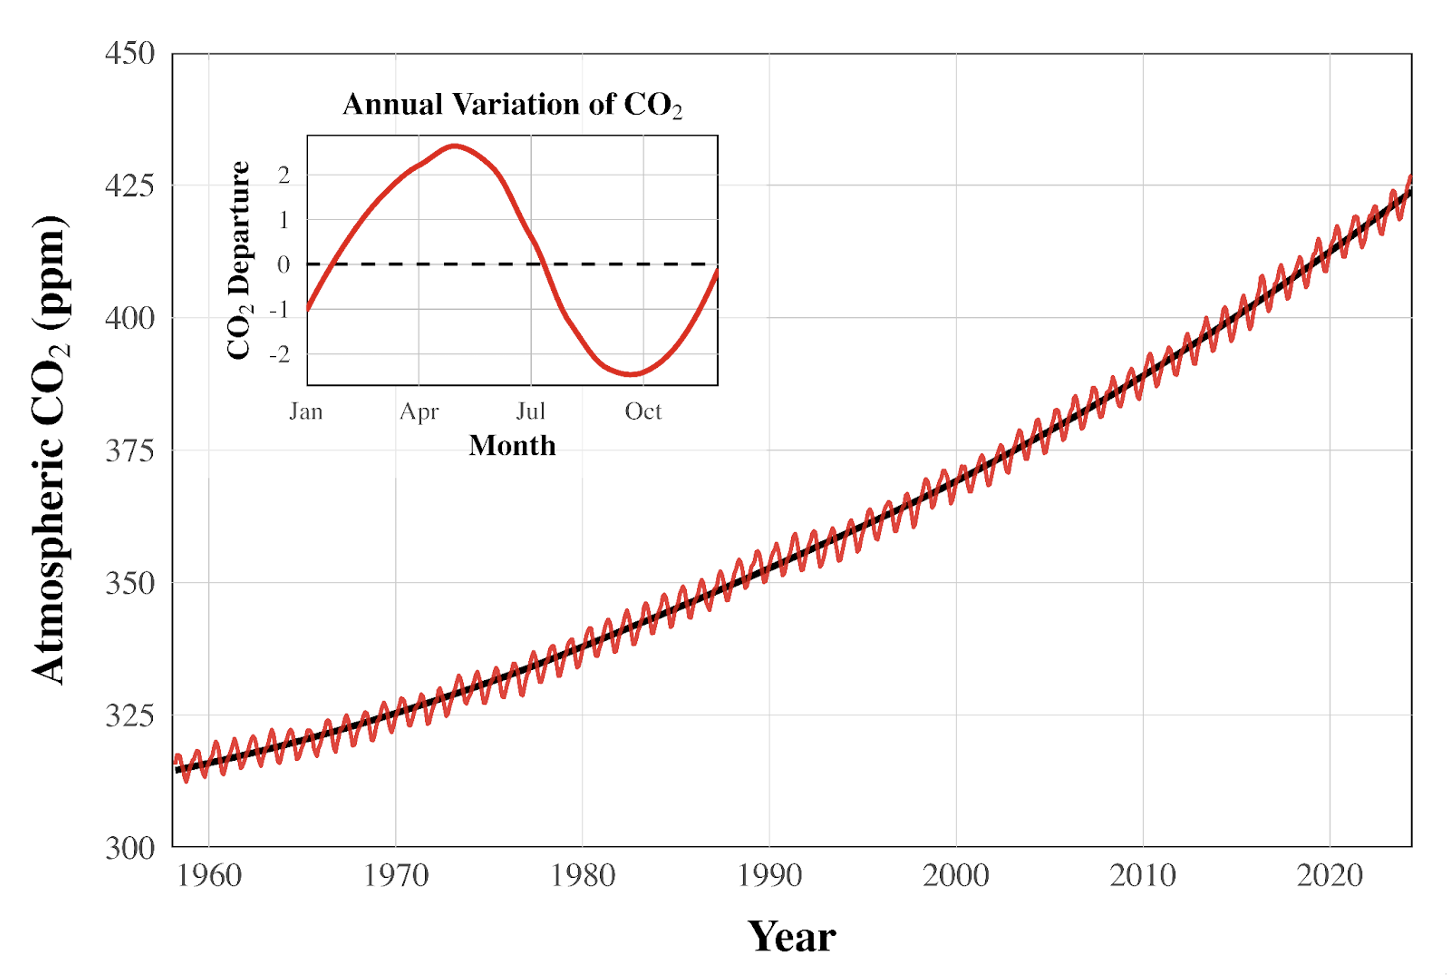
\includegraphics[width=1\textwidth]{ /Users/robertjdellinger/Documents/Github/CSUN-masters-thesis/figures/chapter1/Fig_1_1_Atmospheric_CO2.png }
  \caption[Monthly atmospheric CO\textsubscript{2} concentration (ppm), Mauna Loa Observatory, Hawaii (1958--2024).]{Keeling curve with annual variation inset (differences from annual average) illustrating planetary-level photosynthesis and respiration exerting an influence on atmospheric CO\textsubscript{2}. Data from NOAA Global Monitoring Laboratory.}
  \label{fig:atmospheric_co2}
\end{figure}

As the atmospheric carbon dioxide (CO\(_2\)) concentration continues to surpass the limits of the earth system, marine organisms will be forced to endure profound transformations of the environment, from shifts in temperature to altered seawater biogeochemistry that will layer on top of natural variability within ecosystems (Figure\textasciitilde{}\ref{fig:atmospheric_co2}) (Pörtner \& Farrell, 2008; Richardson et al., 2023). Since the beginning of the 20th century, the global mean sea surface temperature (SST) has increased by 0.88 {[}0.68--1.01{]}\(^\circ\)C, and is further projected to warm by 2.89\(^\circ\)C {[}2.01--4.07\(^\circ\)C{]} at the end of the century, which surpasses the thermal tolerance limits of many marine species (Bay, Rose, Logan, \& Palumbi, 2017; Fox-Kemper et al., 2021; Kikstra et al., 2022). Concurrently, the ocean has absorbed approximately \(30\%\) of all anthropogenic CO\(_2\) emissions (Feely et al., 2004), resulting in significant alterations in seawater pH (Equations:\textasciitilde{}\ref{eq:co2_dissolution}, \ref{eq:bicarbonate_equilibrium}, and \ref{eq:carbonate_equilibrium}).

\begin{equation}
\begin{aligned}
\ce{CO2(g)} \\[-0.8em]
\ce{\downarrow} \ \ \ \ \ \\[-0.8em]
\ce{CO2(aq)}
\end{aligned}
\label{eq:co2_dissolution}
\end{equation}

\begin{equation}
\ce{CO2(aq) + H2O(l) <=> H+ (aq) + HCO3^- (aq)}
\label{eq:bicarbonate_equilibrium}
\end{equation}
\vspace{-\baselineskip}
\begin{equation}
\ce{HCO3^- (aq) <=> H+ (aq) + CO3^{2-} (aq)}
\label{eq:carbonate_equilibrium}
\end{equation}

The equation above illustrates the reaction that unfolds as CO\(_2\) diffuses into seawater to produce carbonic acid (H\(_2\)CO\(_3\)) and subsequently dissociates into bicarbonate ions (HCO\(_3^-\)) and hydrogen ions (H\(^+\)) (Feely et al., 2004)(Equations:\textasciitilde{}\ref{eq:co2_dissolution}, \ref{eq:bicarbonate_equilibrium}, and \ref{eq:carbonate_equilibrium}). Further dissociation of bicarbonate ions engenders additional hydrogen ions (H\(^+\)) alongside carbonate ions, effectively increasing the acidity of seawater.

Ocean warming (OW) and ocean acidification (OA) are not isolated phenomena; they share a common origin and are byproducts of an extract economy built on fossil fuel (Wolff et al., 2015; Licker et al., 2019; Healy et al., 2019). In a rapidly changing world, their combined impacts on organismal physiology necessitate a more nuanced understanding as multiple drivers of change will act interactively (Côté et al., 2016; Darling \& Côté, 2008). Moreover, the impacts of OW and OA will not be consistent across geographic regions, leading to differential effects that will modify already variable spatial and temporal environments (Gruber, 2011; Kroeker et al., 2016). Organisms undergoing physiologically stressful conditions that result in elevated metabolic costs and restricted aerobic capacity (limited aerobic scope) could be further limited by the inability to counteract additional stressors, yet these instances are dependent upon magnitude and context (Sokolova, 2013; Todgham \& Stillman, 2013). For example, a +12°C thermal shock improved the hypoxia tolerance of tidepool sculpins (Oligocottus maculosus), while a +15°C shock significantly reduced the resilience of the fish to additional stressors (Todgham et al., 2005; Todgham \& Stillman, 2013). Thus building a mechanistic understanding of how the combined impacts of OW and OA affect marine organisms across an environmental gradient is integral for reliable projections of how climate change may impact marine species (Kroeker et al., 2017; Pörtner, 2012a). Despite the increasing emphasis on multi-driver and multi-species studies, a mechanistic understanding of the nonlinear responses regarding the interactive effects of OA and OW remains a critical knowledge gap (Kroeker et al., 2017).

The coastal and adjacent waters of the northeastern Pacific Ocean, known as the California Current System (CCS), present a particularly advantageous living laboratory for enhancing our capacity to comprehend the impacts of multiple drivers of global change on organismal physiology and energetics (Hofmann, Evans, Kelly, Padilla-Gamiño, Blanchette, Washburn, Chan, McManus, Menge, \& Gaylord, 2014; Somero et al., 2016). The CCS is an extensively-studied marine ecosystem where long-term data and research illustrate the impacts of climatic variability (e.g.~Pacific Decadal Oscillation and El Niño Southern Oscillation (García‐Reyes \& Largier, 2012)) on abiotic factors, such as temperature and carbonate chemistry, with associated changes already impacting organismal performance (Chavez et al., 2003; Connolly \& Roughgarden, 1998; Feely et al., 2008, 2012; Kroeker, Gambi, et al., 2013; Mekkes et al., 2021; Somero et al., 2016). Temperature logger (Onset Tidbit V2 Temp Data Logger; Onset Computer Corp.~UTBI-001) data from Multi-Agency Rocky Intertidal Network (MARINe) and Partnership for Interdisciplinary Studies of Coastal Oceans (PISCO) bolted to the substrate within a long-term intertidal monitoring site at Port Fermin, Los Angeles, CA from August--September 2022, reveal an average ocean water temperature of 17.31°C and a maximum ocean water temperature of 23.79°C during high tide, contrasting with a slightly higher mean aerial temperature of 17.41°C, which can soar to a maximum of 33.73°C during low tide (Multi-Agency Rocky Intertidal Network (MARINe) et al., 2023). These findings highlight the natural variability and acute thermal stress that intertidal organisms are subjected to within the southern California Bight region of the CCS, particularly during aerial exposure. Furthermore, despite the inherent natural variability present within California coastal ecosystems, a comprehensive analysis of the measurements of coastal ocean temperatures in the Southern California Bight over the past century (1917-2017) reveals significant increases in nearshore temperatures, delineating a warming trend of 1.24 ° C per century at the surface and 1.67 ° C per century in bottom waters (Rasmussen et al., 2020). Moreover, the longest running record of carbonate system dynamics in the CCS reveals a 37-year record of ocean acidification in the Southern California region with an expected decrease in pH of -0.15 ± 0.01 units per century (Wolfe et al., 2023). These concurrent changes and inherent variability make the CCS a particularly important location for studying the impacts of multiple global changes.

\section*{Comparative Physiology as a Means to Delineate Responses to Multiple Drivers of Change}\label{comparative-physiology-as-a-means-to-delineate-responses-to-multiple-drivers-of-change}
\addcontentsline{toc}{section}{Comparative Physiology as a Means to Delineate Responses to Multiple Drivers of Change}

The integration of thermal performance curves (TPC) with the metabolic theory of ecology, which posits that the energetic expenditure of organisms is fundamentally linked to environmental temperatures, enables ecologists to forecast changes in species distributions and community structures as global temperatures continue to rise against a backdrop of acidification (Brown et al., 2004; Kroeker et al., 2017; Kroeker, Gaylord et al., 2014). The use of performance curves can help to quantify the relationship between physiological rates across an environmental gradient and can allow for comparative assessments across different biological rates and environmental conditions (Becker \& Silbiger, 2020; Kroeker, Gaylord, et al., 2014; Schulte et al., 2011; Silbiger et al., 2019). By comparing the physiological rates of organisms across environmental gradients, it becomes possible to effectively quantify and compare the constraints, metrics, and tolerance limits of species (Hochachka \& Somero, 2002). In addition, thermal performance curves have been proposed to bridge the knowledge gap among multiple stressor interactions and aspects of global change, as they delineate the relationship between physiological rates across a range of temperatures and allow for the integration of additional abiotic factors, such as salinity, oxygen availability, and pH (Gaylord et al., 2015; Huey \& Stevenson, 1979; Schulte et al., 2011; Sinclair et al., 2016).

Thermal performance curves represent a univariate function (dose-response relationship) that empirically quantifies how measurements of a physiological system occur in relation to varying levels of an environmental factor, from single-molecule (e.g., enzyme kinetics) to organismal-level rates (e.g., consumption rate, respiration rate, growth rate) (Figure 1.2). As temperature increases, biochemical and physiological rates increase exponentially until peaking at a species-specific optimal temperature; further increases in temperature beyond the optimum lead to rapid decreases in performance rate (also known as the Arrhenius Breakpoint; (Schulte, 2015) and eventually protein denaturation, growth inhibition, and reductions in fitness (Pörtner \& Knust, 2007; Schulte, 2015; Somero, 1995). Near the upper and lower limits of an organism's thermal niche, where temperatures reach levels high or low enough to denature crucial metabolic enzymes, and at which locomotory activity becomes disorganized, metabolic performance gradually decreases to zero, leading to the formation of unimodal thermal performance curves (Schoolfield et al., 1981; Sharpe \& DeMichele, 1977; Somero, 1995). The dynamics described are encapsulated in the Sharpe--Schoolfield model, an extension of the Boltzmann--Arrhenius model, which extrapolates the kinetic effects of temperature on cellular processes to the organismal level, as described by \eqref{eq:sharpeschoolfieldfull}:

\begin{equation}
\label{eq:sharpeschoolfieldfull}
R(T) = \frac{R_{T_{\text{ref}}} \cdot e^{\frac{-E_a}{k_B} \left( \frac{1}{T} - \frac{1}{T_{\text{ref}}} \right)}}
{1 + e^{\frac{E_l}{k_B} \left( \frac{1}{T_l} - \frac{1}{T} \right)} + e^{\frac{E_h}{k_B} \left( \frac{1}{T_h} - \frac{1}{T} \right)}}
\end{equation}

\noindent
Wherein:

\begin{itemize}
  \item $R(T)$: Metabolic rate of a biological process as a function of temperature
  \item $R_{T_{\text{ref}}}$: Baseline metabolic rate at the reference temperature $T_{\text{ref}}$
  \item $E_a$: Activation energy in electron volts (eV)
  \item $E_l$: Low-temperature activation energy in electron volts (eV)
  \item $E_h$: High-temperature activation energy in electron volts (eV)
  \item $k_B$: Boltzmann constant, approximately $8.62 \times 10^{-5}$ eV K$^{-1}$
  \item $T$: Absolute temperature (K)
  \item $T_h$: High-temperature threshold at which $\frac{1}{2}$ of the enzymes are active
  \item $T_l$: Low-temperature threshold at which $\frac{1}{2}$ of the enzymes are active
  \item $T_{\text{ref}}$: Standardization temperature in absolute temperature (K)
\end{itemize}

Thermal performance curves are typically left-skewed and parabolic, encompassing several metrics including, but not limited to, a thermal optimum (\(T_{\text{opt}}\))---the temperature at which the maximum rate of performance is achieved---(\(R_{\text{max}}\)), representing the maximal rate of performance, and (\(T_{\text{br}}\)), which denotes the thermal breadth: the range where performance spans \(80\%\) of the maximal rate (Fig.\textasciitilde1.1). Additionally, the critical thermal minimum (\(CT_{\text{min}}\)) and critical thermal maximum (\(CT_{\text{max}}\)) values signify the upper and lower thermal thresholds that organisms can tolerate \ref{fig:tpc_conceptual_diagram} (Huey \& Kingsolver, 1989; Huey \& Stevenson, 1979; Schulte et al., 2011). The tolerance thresholds and corresponding ranges are determined by an organism's capacity to withstand sublethal and lethal conditions via organismal-level and molecular-level responses, such as utilizing anaerobic metabolism and heat shock protein induction (Somero, 2022; Tomanek \& Somero, 2002). It has been shown that exposure to concurrent drivers of ecological change, like OA, will incur physiological costs and limit an organism's aerobic scope, thereby reducing the breadth of performance and, consequently, thermal limits (Gaylord et al., 2015; Pörtner, 2010; Pörtner et al., 2017; Pörtner \& Farrell, 2008).

\newpage

\begin{figure}[ht]
  \centering
  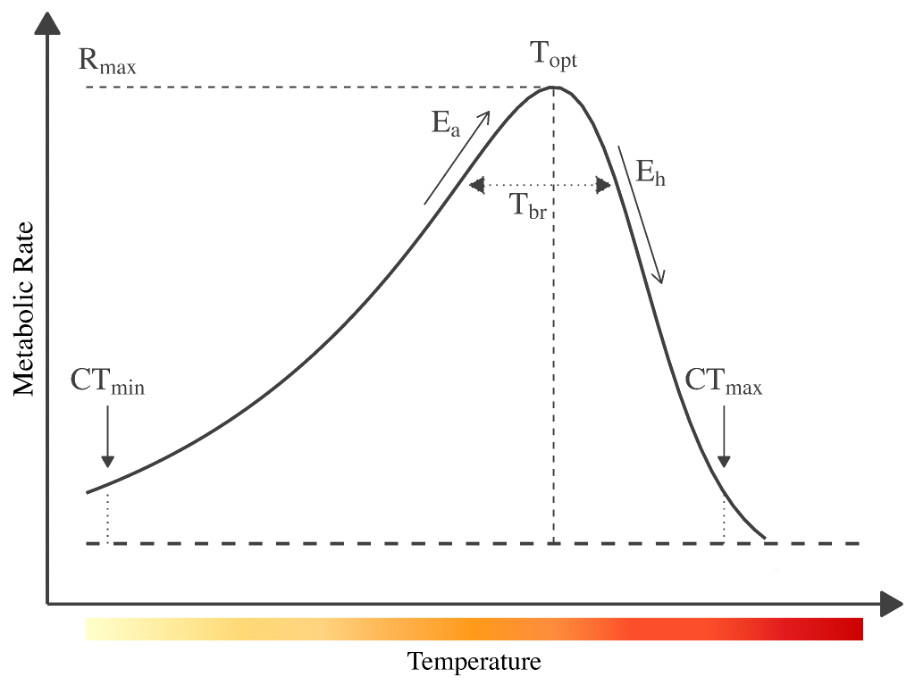
\includegraphics[width=0.9\textwidth]{ /Users/robertjdellinger/Documents/Github/CSUN-masters-thesis/figures/chapter1/Fig_1_2_TPC_Conceptual_Diagram.png }
  \caption[Conceptual diagram of a thermal performance curve (TPC).]{Figure 1.2. Conceptual diagram of a thermal performance curve (TPC) for metabolic rates across a range of temperatures based on the Sharpe--Schoolfield model (Schoolfield et al., 1981; Sharpe \& DeMichele, 1977). The dashed vertical line in the center indicates the thermal optimum ($T_{\text{opt}}$), while the dashed horizontal line at the highest point of the curve denotes the highest metabolic rate ($R_{\text{max}}$). The dotted vertical line at each end of the curve denotes the thermal limits, including the critical thermal minimum ($CT_{\text{min}}$) and critical thermal maximum ($CT_{\text{max}}$). The arrow parallel with the increasing slope of the curve represents the activation energy ($E_a$), while the arrow parallel with the downward slope of the curve, beyond the optimum temperature, represents the deactivation energy ($E_h$) of the curve. The thermal breadth range ($T_{\text{br}}$) is denoted by the horizontal dotted line segment with arrows at each end spanning the length of the curve corresponding to temperatures at which the metabolic rate exceeds 80\% of the peak performance. (Created using the rTPC package, Padfield et al., 2021.)}
  \label{fig:tpc_conceptual_diagram}
\end{figure}

Employing a performance curve approach, this research delineated how OA affects the energetic demands (O\(_2\) consumption) of the black turban snail, (\textit{Tegula funebralis}) across a gradient of temperature. The impact of OA is particularly significant for calcifying organisms, such as gastropods, that experience reductions in calcification rates, more so than other calcifying groups (Bellwood et al., 2004; Kroeker, Kordas, et al., 2013). As an abundant herbivore ubiquitous across intertidal ecosystems along the CCS, \textit{T. funebralis}, reaching population densities of over 1000 individuals per m\(^{2}\) in the Northern West Coast of the United States, plays a crucial role in the energy flow through coastal food webs (Paine, 1971), directly affecting algal communities and serving as prey for a variety of predators (Paine, 1966, 1971, 1980). Understanding these interactive effects on herbivores is crucial, as the macroalgal-herbivore interaction is the primary pathway for energy transfer across trophic levels (O'Connor et al., 2009). \textit{T. funebralis} is also a prime subject for OW research due to its tolerance across a broad temperature range, compared to lower intertidal congeners within the genus \textit{Tegula}, which has facilitated its widespread distribution across the mid-high intertidal zone spanning from Vancouver Island, British Columbia, Canada (51\(^\circ\)N), to San Geronimo Island, Baja California, Mexico (30\(^\circ\)N) (Fawcett, 1984; Frank, 1975; Gravem \& Morgan, 2017; Morris et al., 1980; Nielsen, 2001). Furthermore, \textit{Tegula funebralis} follows the temperature-size rule (sensu Angilletta \& Dunham), exhibiting declines in body size with increasing temperatures along both latitudinal and intertidal zonation gradients, with larger individuals along the Northern regions of its distribution and smaller individuals along the Southern region of its distribution (Byers \& Mitton, 1981; Cooper \& Shanks, 2011; Frank, 1975). The outcomes of this research help reveal how changes in vital rates could affect population dynamics and, consequently, ecosystem processes in our changing oceans (Kroeker et al., 2017). Investigating the interactive effects of OA and OW is essential to enhancing our understanding of the physiological capacities of marine organisms to withstand environmental change, and thereby integral for conservation, management, and policy.

\chapter*{\texorpdfstring{Chapter 2: Ocean acidification alters thermal performance metrics and increases energetic demand in the intertidal gastropod, \textit{Tegula funebralis}}{Chapter 2: Ocean acidification alters thermal performance metrics and increases energetic demand in the intertidal gastropod, }}\label{chapter-2-ocean-acidification-alters-thermal-performance-metrics-and-increases-energetic-demand-in-the-intertidal-gastropod}
\addcontentsline{toc}{chapter}{Chapter 2: Ocean acidification alters thermal performance metrics and increases energetic demand in the intertidal gastropod, \textit{Tegula funebralis}}

\section*{Introduction}\label{introduction}
\addcontentsline{toc}{section}{Introduction}

The stability of marine ecosystems is undergoing significant changes in energy dynamics due to the escalating physiological costs imposed by a rapidly changing environment. Extractive industries have fundamentally restructured the global carbon cycle by combusting previously sequestered CO\(_2\) into the atmosphere, triggering a global physicochemical shift within the oceans (Wolff et al., 2015). The ocean has served as the primary reservoir for absorbing these planetary changes, uptaking approximately a quarter of all anthropogenic-induced CO\(_2\) emissions (Doney et al., 2009; Feely et al., 2004) and a thermal energy influx of approximately 10.9 Zetta Joules (Cheng et al., 2023), resulting in the dual processes of ocean acidification and warming (OA \& OW). These changes equate to a rate of change unprecedented in geological history over the past 56 million years with diminutions in pH corresponding to a 30\% increase in ocean acidity and a temperature increase energetically analogous to multiple nuclear detonations every few seconds (Burger et al., 2020; Friedlingstein et al., 2022). This stark analogy underscores the massive scale of energy redistribution within marine environments, which is altering the energetic demands of individual organisms and cascading to affect the complex network of species interactions that regulate populations and structure communities (Odum, 1968; Paine, 1980). These rapidly changing conditions force evolutionary responses of species within relatively short ecological time frames. Thus, deciphering the energetic demands imposed by concurrent changes in the abiotic environment is crucial for understanding how organisms maintain physiological homeostasis in changing environments (Somero, 2020; Somero et al., 2016). Ultimately, understanding the interactive effects of OA and OW remains an utmost priority for science, conservation, and policy.

Ocean warming will affect virtually all marine ecological processes as changes in temperature have direct impacts on the temperature dependence of all biological and chemical processes (Brown et al., 2004; Hochachka \& Somero, 2002; Hofmann \& Todgham, 2010; Huey \& Stevenson, 1979; Levins, 1968; Schmidt-Nielsen, 1997; Somero, 2002). These impacts will increase the kinetic speed of biochemical reactions, modify internal acid-base regulation (variations in pH \(\sim\) 0.017 per \(^\circ\)C of body temperature change), modulate metabolic pathways, and shift the equillibria of constructing biological structures (Pörtner, 2012a; Somero et al., 2016). Through doing so, changes in temperature ultimately impact energetic demands and thus the fitness and distribution patterns of marine species (Huey \& Kingsolver, 1989). In ectothermic species, cellular respiration is governed by the ability to withstand temperature, with eurythermal species capable of surviving across a wide range of temperatures, or stenothermal, restricted to a narrow temperature range. For example, temperature changes differentially affect the metabolic demands of intertidal gastropods in the genus \textit{Tegula}, with the species \textit{T. funebralis} situated within the high-mid intertidal zone experiencing higher metabolic rates due to their greater tolerance across a range of temperatures, compared to subtidal congeners \textit{T. brunnea} and \textit{T. montereyi}, which experience relatively less temperature variability and lower thermal tolerances (Byers \& Mitton, 1981; Frank, 1975; Somero, 2011; Tomanek \& Somero, 1999).

Ocean acidification will also interact against a backdrop of warming to affect the metabolic activity of marine organisms, posing a unique threat to marine calcifiers and potentially elevating the energetic costs associated with metabolic activity. Similar to temperature increases, changing acidity will influence the internal acid-base concentration gradients, exerting energetic costs on maintaining cellular homeostasis (Bozinovic \& Pörtner, 2015; Michaelidis et al., 2005b; Somero, 2020). Moreover, changes in seawater carbonate chemistry elevate the energetic costs associated with calcification and possibly undermine the formation of calcified structures within marine organisms (Mekkes et al., 2021; Spalding et al., 2017), yet, in contrast, some marine calcifiers may be able to maintain or even elevate calcification in response to OA (e.g., calcite versus aragonite, see Barclay et al., 2019). For example, gastropods like \textit{Tegula funebralis} and \textit{Nucella ostrina} show cryptic variability in calcification under ocean acidification, with \textit{T. funebralis} experiencing significant shell integrity reduction, while \textit{N. ostrina} remains relatively unaffected, indicating species-specific responses to energetic demands (Barclay et al., 2019; Gaylord et al., 2019).

The dual pressures of OA and OW pose significant challenges for coastal marine organisms in highly stochastic physical environments, often facing natural variability that exceeds future projections (Helmuth, 1999; Jellison et al., 2016; K. Wolfe et al., 2020). The California Current System provides a living laboratory of climatic changes that allows us to understand how organisms thrive and persist amidst the inherent variability in seawater carbonate chemistry and temperature (Hofmann et al., 2014; Gaylord et al., 2014; Somero et al., 2016). Intertidal organisms, for example, experience significant temperature changes, as high as 25\(^\circ\)C within a single tidal cycle, with Southern California intertidal ecosystems displaying aerial and aquatic temperatures ranging from 12.2 to 45.05\(^\circ\)C (Davis, 2001; Helmuth et al., 2016; Helmuth, 1998; Tomanek \& Somero, 1999; K. Wolfe et al., 2020). Additionally, diurnal variations in the carbonate chemistry of intertidal rock pools, which become isolated at low tide, can cause significant pH fluctuations of up to \(\sim\!1.11\ \mathrm{pH}_\mathrm{T}\) units within a single tide cycle (Jellison et al., 2016, 2022; Kunze et al., 2021; Kwiatkowski et al., 2016; Silbiger \& Sorte, 2018). Community-level metabolic activity adds to this variability during conditions when CO\(_2\) accumulation from respiration surpasses photosynthetic activity, leading to further reductions in pH throughout nighttime dissolution lows and biophysical feedback loops (Fields \& Silbiger, 2022; Gaylord et al., 2019; Kwiatkowski et al., 2016; Silbiger \& Sorte, 2018). Thus, intertidal ecosystems exhibit drastic variability that offer a glimpse into the future, providing insights on how organisms respond to changing environments.

A key goal of ecology is to uncover patterns and mechanisms within ecological communities (Levins, 1992). One of these objectives is to determine whether the combined effects of multiple stressors will act interactively through additive, synergistic, or antagonistic interactions---and of prime importance is whether concurrent global changes (such as OA and OW) will overlay to amplify environmental change (Côté et al., 2016; Darling \& Côté, 2008). Thermal performance curves (TPCs) have been suggested to fill this gap of uncertainty, as they empirically characterize the relationship between biological rates of performance across a gradient of temperatures (Angilletta, 2009; Levins, 1969; Schulte et al., 2011). Additionally, TPCs facilitate the integration of various abiotic factors, enabling comparative physiological metrics, such as metabolic rates and thermal tolerances, between populations and species. This integration serves as a ``crystal ball'' (sensu Somero, 2011) for predicting the impacts of global change (Dowd et al., 2015; Silbiger et al., 2019; Sinclair et al., 2016). The Metabolic Theory of Ecology (MTE) provides a mechanistic framework for integrating TPCs to changes in energetic expenditure, interlinking ecological drivers and organismal metabolism, and positing that metabolic rates are governed by temperature-dependent enzyme reaction rates, the size of the organism, and the stoichiometry of an organism's biochemical processes (Brown et al., 2004; Gillooly et al., 2001). Organism-level aerobic respiration (O\(_2\) consumption) provides a direct measure of metabolic rate and serves as a proxy for cellular respiration because oxygen is essential for the production of ATP through oxidative phosphorylation, thus allowing us to estimate the energetic expenditure of marine organisms. By analyzing respiration rates through a TPC approach, I can delineate the relationship between temperature and metabolic demand alongside the comparative assessment of additional abiotic factors of global change such as OA.

For this study, I investigated physiological energetics of the black turban snail \textit{Tegula funebralis}, a eurythermal intertidal gastropod situated within the thermally stressful high intertidal zone of the Pacific Northwest, United States (\(-0.5\) m to 1.5 m, Tomanek \& Somero, 1999), to explore the interactive effects of ocean acidification on respiration rates across a gradient of temperature in a controlled laboratory setting. \textit{T. funebralis}, distributed along the west coast of North America from Canada (51\(^\circ\)N) to Mexico (30\(^\circ\)N) (Morris et al., 1980), was selected to implore this question because of its ubiquity across intertidal ecosystems (ranging in densities of up to \(>1000~individuals~per~m^2\) in the northern distribution and ranging from 10--100 individuals per m\(^2\) in the southern distribution (Jones \& Long, 2018; Pacific Rocky Intertidal Monitoring, 2023; Paine, 1971)), its important role as a macroalgal herbivore/detritivore in influencing energetic flow within intertidal food webs (up to 60\% energy transfer from primary producers to primary consumers, see Paine, 1969; Paine, 1971), observed body size declines associated with increasing temperatures over the past few decades, consistent with the temperature-size rule (Elahi et al., 2020), and its particular vulnerability to calcification reductions and anti-predator behavioral impairment due to OA (Barclay et al., 2019; Jellison et al., 2016).

Within this research, I posed the question: how does exposure to decreased pH influence thermal performance and energetic expenditure of the intertidal gastropod, \textit{Tegula funebralis}? I hypothesized that the thermal optimum (\(T_{\text{opt}}\)) and critical thermal maximum (\(CT_{\text{max}}\)) for respiration rates will shift towards lower temperatures, indicating a reduced ability to sustain optimal metabolic activity in the face of ocean acidification (Figure\textasciitilde{}\ref{fig:tpc_hypothesis_schematic}). Additionally, I expect a decrease in the thermal breadth of the curve (\(T_{\text{br}}\)), indicating a narrower range of temperatures at which the gastropod can effectively maintain respiratory rates (Figure\textasciitilde{}\ref{fig:tpc_hypothesis_schematic}). Consequently, I anticipate that \textit{Tegula funebralis} will exhibit increased energetic expenditure as a function of rising sea temperatures and lowered pH levels, with more pronounced changes at temperature extremes, thereby reflecting a higher cost of maintaining homeostasis under elevated stress. Predicting the consequences of concurrent global changes using a thermal performance curve approach will enable me to make generalized hypotheses regarding how ocean acidification may impact organismal-level processes and infer how these changes will scale up to affect ecosystem function (e.g., net primary productivity, calcification, etc.).

\newpage

\begin{figure}[H]
  \centering
  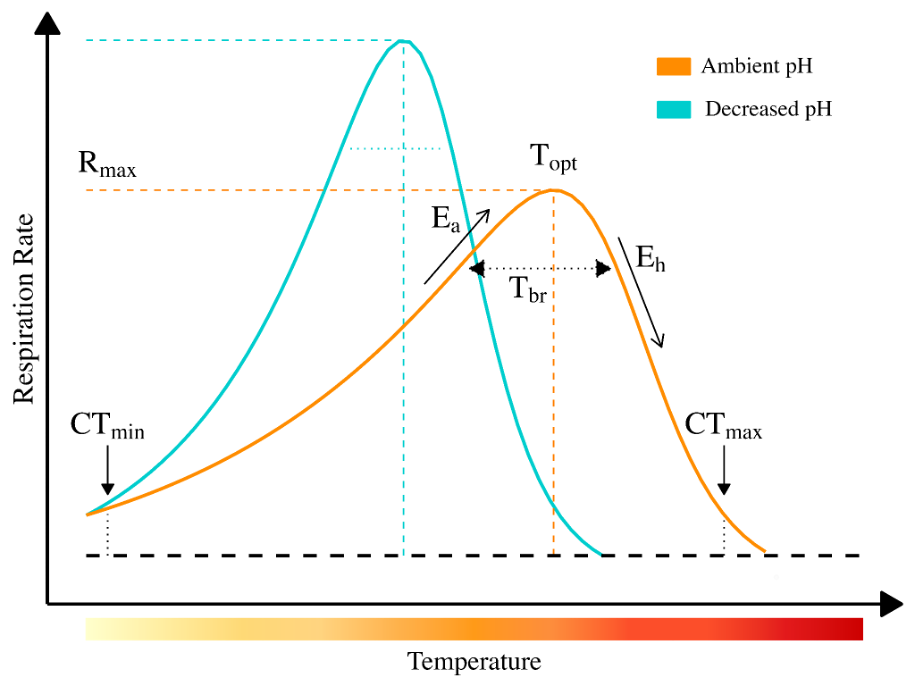
\includegraphics[width=0.9\textwidth]{ /Users/robertjdellinger/Documents/Github/CSUN-masters-thesis/figures/chapter2/Fig_2_1_TPC_Hypothesis_Schematic.png }
  \caption[Hypothesis schematic diagram of TPCs under ambient and low pH conditions.]{Hypothesis schematic diagrams of TPCs for respiration rates across a range of temperatures with exposure to either ambient or low pH conditions based on the Sharpe--Schoolfield model (Schoolfield et al., 1981; Sharpe \& DeMichele, 1977). The dashed vertical lines indicate the optimal temperatures ($T_{\text{opt}}$) for each curve, with a reduction in the thermal optimum at decreased pH, while the dotted vertical lines denote the thermal limits, including the minimum critical temperature ($CT_{\text{min}}$) and maximum critical temperature ($CT_{\text{max}}$), with constrictions hypothesized at lower pH. The arrow pointing upwards (parallel with the increasing slope of the curve) represents the activation energy ($E_a$) and predicts an increased activation energy under decreased pH, while the arrow pointing downwards (past the optimum) represents a steeper deactivation energy ($E_h$) with exposure to decreased pH. The dashed horizontal arrow denotes the highest metabolic rate ($R_{\text{max}}$) with a hypothesized increase in energetic requirements (respiration rate $\sim$ O$_2$ consumption) under decreased pH. The thermal breadth range ($T_{\text{br}}$, 80\% of peak performance) is denoted by the horizontal dotted line segment with arrows at each end and hypothesized to constrict in range throughout exposure to decreased pH.}
  \label{fig:tpc_hypothesis_schematic}
\end{figure}

\section*{Methods}\label{methods}
\addcontentsline{toc}{section}{Methods}

\subsection*{Experimental Design}\label{experimental-design}
\addcontentsline{toc}{subsection}{Experimental Design}

Using a mesocosm system, I exposed \textit{Tegula} to one of eight temperature treatments {[}ranging from 12\(^\circ\)C to 26\(^\circ\)C at 2\(^\circ\)C intervals; \(n=8\){]} and to one of two pH treatments {[}7.9 pH\(_\mathrm{T}\) (ambient); 7.7 pH\(_\mathrm{T}\) (low); \(n=2\){]}, resulting in sixteen temperature by pH combinations (\(n=4\) \textit{Tegula} per treatment). After a 7-day tank adjustment period and a 10-day exposure to experimental treatments, respiration rates were measured for each individual snail (\(n=60\)). Furthermore, rates of oxygen consumption were converted to J g\(^{-1}\) h\(^{-1}\) to translate metabolic changes to changes in energetic requirements.

Temperature (12--26\(^\circ\)C) and pH\(_\mathrm{T}\) (7.7 and 7.9) ranges were chosen to mirror the local variability that \textit{Tegula} experience within intertidal ecosystems of the Southern California Bight. Data from a subtidal monitoring station in Newport Beach, CA, showed seawater temperatures ranging from 11.7\(^\circ\)C to 25.2\(^\circ\)C over the past three years (Carter, 2022), with an average of 21\(^\circ\)C during the summer months (August--September) when my study was conducted (Fig.\textasciitilde3B, Appendix 1A). Moreover, offshore pH\(_\mathrm{T}\) recorded at a subtidal shore station in Newport Beach, CA revealed a mean pH\(_\mathrm{T}\) of 8.01 \(\pm\) 0.07, with minima reaching 7.3 (Figure\textasciitilde{}\ref{fig:study_site_map}, Appendix B1). Previous research has shown tidepool pH\(_\mathrm{T}\) variability within the Southern California Bight to range from approximately 7.5 to 8.7 over a diel cycle compared to adjacent ocean diel variability ranging from 7.9 to 8.3 (Silbiger and Sorte, 2018), highlighting the relevance of the chosen pH\(_\mathrm{T}\) levels 7.7 and 7.9.

\subsection*{Species Collection and Adjustment}\label{species-collection-and-adjustment}
\addcontentsline{toc}{subsection}{Species Collection and Adjustment}

Black turban snails (\(n=45\)) were collected haphazardly from tidepools in Point Fermin, San Pedro, CA (Figure\textasciitilde{}\ref{fig:study_site_map}) in August 2022 (under permit CDFW SCPID: S-220520002-22054-001) at low tide. Upon collection, each snail was measured for shell width (\(\pm\) 0.001 mm) using Vernier calipers. To minimize variability resulting from mass-specific metabolic rate, only individuals ranging from 19--24 mm in shell width (\(>18 mm\) mature individuals \(\sim\) 10 years old; Paine, 1971) were selected for the experiment. Organisms were transported to California State University, Northridge, in a wet insulated container. Snails were weighed for blotted wet mass (g) using an electronic balance to the nearest 0.0001 g, measured for volume (mL) using volumetric displacement, and tagged for identification using a FloyTag placed at the apex of the dorsal side of the shell with CorAffix\textsuperscript{\textregistered} cyanoacrylate adhesive.

\begin{figure}[H]
  \centering
  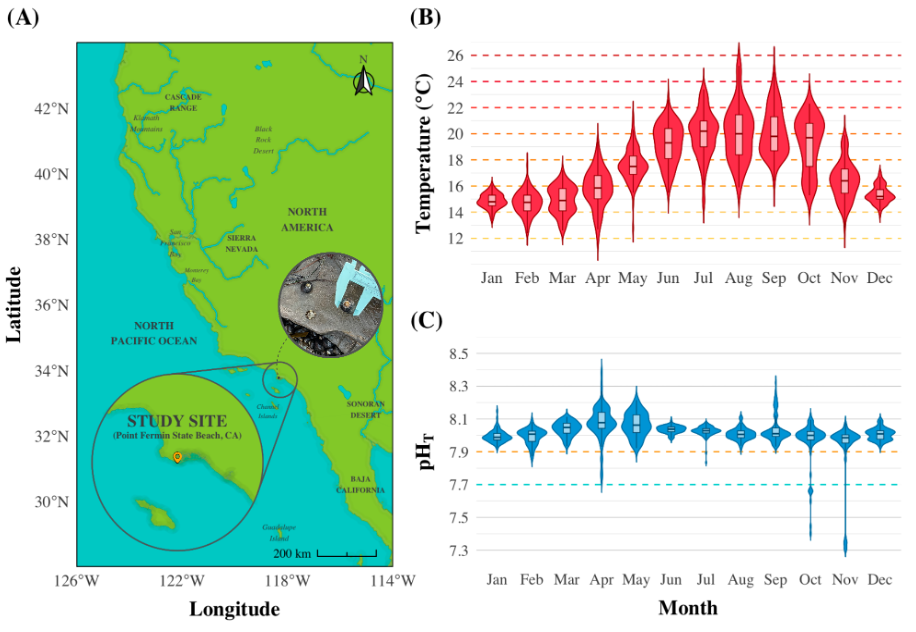
\includegraphics[width=6.25in]{ /Users/robertjdellinger/Documents/Github/CSUN-masters-thesis/figures/chapter2/Fig_2_2_Study_Site_Map.png }
  \caption[Study site location map and associated SST and pH\textsubscript{T} variability.]{Study site location map and associated temporal variability within sea surface temperature (SST) and pH\textsubscript{T} at a nearby shore station (Newport Beach, CA). (A) Annotated map of the Pacific Coast with an inset zooming into the study site at Point Fermin State Beach, California (33.7056$^\circ$N, 118.2935$^\circ$W), created in R using \texttt{raster}, \texttt{sf}, \texttt{ggmap}, and \texttt{ggmapinset} (Hijmans et al., 2015; Kahle \& Wickham, 2013; Pebesma, 2018; Suster, 2023). (B) Violin plot showing the monthly frequency distribution of daily average SST data spanning 2020 to 2023 from Newport Beach, CA at a nearby shore station approximately $\approx$ 23 km from the study site. Horizontal dashed lines indicate experimental temperature treatments ranging from 12$^\circ$C--26$^\circ$C by 2$^\circ$C increments. (C) Analogously, the violin plot for seawater pH\textsubscript{T} showcases the monthly frequency distribution of daily average values on the total scale, spanning 2020 to 2023 at the same shore station. The horizontal dashed lines highlight the experimental treatment levels (pH\textsubscript{T} 7.9 (ambient) and 7.7 (low)). Data for these plots were provided by the Southern California Coastal Ocean Observing System and the Shore Stations Program at the Scripps Institution of Oceanography, supported by the California Department of Parks and Recreation, Natural Resources Division, Award \#C1670003.}
  \label{fig:study_site_map}
\end{figure}

Each black turban snail was randomized and assigned to one of 16 experimental aquaria, with four individuals per aquarium. All aquaria were set to measured seawater temperature and seawater pH from the time of collection in order for the snails to adjust to tank conditions. Temperature was set to 16\(^\circ\)C and pH\(_\mathrm{T}\) was set to 7.9. The next day, snails were moved to a pH\(_\mathrm{T}\) treatment of either 7.9 or 7.7. On the second day in the mesocosm system, snails slated for temperature conditions either higher or lower than 16\(^\circ\)C were increased or decreased at a gradual temperature change of 2\(^\circ\)C day\(^{-1}\) such that all snails reached their treatment temperature and pH after seven days. Throughout the adjustment and the subsequent experimental period, all snails were fed a three-inch in diameter circle of fresh giant kelp (\textit{Macrocystis pyrifera}) from nearshore Point Fermin, a highly preferred food (Steinberg, 1985) every three days. This feeding rate was chosen to maintain nutritional consistency of algae and prevent metabolic rate fluctuations due to food availability (Brockington, 2001).

\subsection*{Mesocosm Settings Overview and Maintenance}\label{mesocosm-settings-overview-and-maintenance}
\addcontentsline{toc}{subsection}{Mesocosm Settings Overview and Maintenance}

This experiment was conducted in a closed-loop mesocosm system at California State University, Northridge, using natural seawater collected from the Southern California Marine Institute (SCMI) in San Pedro, CA, and filtered through three filters (20\textasciitilde{}\(\mu\)m, 5\textasciitilde{}\(\mu\)m, and a carbon filter {[}up to 1\textasciitilde{}\(\mu\)m{]}) prior to being introduced into the sump of the mesocosm system. The mesocosm was equipped with experimental tanks (53.9\textasciitilde cm (L) \(\times\) 31.75\textasciitilde cm (W) \(\times\) 34.29\textasciitilde cm (H)) each with individual controls for pH, temperature, light intensity, and water flow. Each aquarium was outfitted with a submersible powerhead pump (Hydor Nano Koralina 240 powerhead, 240 GPH), a 200 or 400W heater (Hydor aquarium heater), a temperature probe (Neptune Systems, \(\pm 0.1^\circ\)C), a pH probe (Neptune Systems, Lab Grade Double Junction, measures pH from \(4.0 to 12.0 \pm 0.1\)), three flow sensors (Apex, FS-25 ¼'' fitting, flow rates from 3--12 GPH (12--24 LPH)), and a continuous temperature logger (HOBO TidBit MX2203, \(\pm 0.2^\circ\)C ). LED lights (Halo Basic M-110) in each tank followed a diurnal light cycle to mimic light levels between local sunrise and sunset conditions. Individual aquaria were programmed to simulate the semi-diurnal tidal patterns that characterize the West Coast of the United States, undergoing two high and two low tide fluctuations within a 24-hour cycle, each lasting six hours, by programming inflow and outflow solenoid valves (Apex Neptune). Flow rates were measured on a daily basis using a graduated cylinder and timer to ensure an inflow of 10\textsubscript{L}h\(^{-1}\), constant total inflow of 10\textsubscript{L}h\(^{-1}\), and a constant outflow drain rate of 15\textsubscript{L}h\(^{-1}\), thereby creating the desired tidal effect and mimicking the biological rhythmicity these organisms would experience in the field.

Temperature and pH were controlled by a stat system using Apex programmable aquaria controllers outfitted with pH and temperature probes (Neptune Systems). Tank temperature was controlled with aquarium heaters while pH levels were regulated through the direct bubbling and mixing of CO\(_2\), facilitated by solenoid valves attached to a CO\(_2\) cylinder. Additionally, a venturi connected to a pump facilitated the mixing of ambient air to stabilize the pH levels in the treatment tanks. Recirculating seawater in the closed-loop system underwent a series of biological and chemical filtration in the central holding reservoir, throughout which seawater was chilled to a temperature of 10\(^\circ\)C (Aqua Logic Delta Star, DS-4 chiller) and bubbled with CO\(_2\)-free air from a Phosban reactor (Phosban 150 Reactor), forcing CO\(_2\) to be off-gassed and returning pH back to ambient conditions prior to recirculating into treatment tanks. Additionally, the recirculating seawater was purified using three 50\textasciitilde{}\(\mu\)m carbon bag filters, eight mesh filters, and an ultraviolet sterilizer (Comet Series 95 Watt Lamp). Weekly water replacements, accounting for approximately 50\% of the total volume, were conducted to prevent the accumulation of metabolic waste and to maintain stable carbonate parameters within the system.

\subsection*{Measurements to Monitor Experimental Seawater Conditions}\label{measurements-to-monitor-experimental-seawater-conditions}
\addcontentsline{toc}{subsection}{Measurements to Monitor Experimental Seawater Conditions}

In addition to the apex-measured pH and temperature conditions, water quality parameters were measured to monitor environmental conditions within the tanks. pH and temperature were measured daily at approximately 9:30 AM to facilitate the calibration of in-tank temperature and pH probes. Discrete temperature readings were acquired using a Thermo Fisher Trace digital thermometer with an accuracy of \(\pm~0.05^\circ\)C, providing measurements to the nearest \(0.001^\circ\)C. In tandem, a Thermo Scientific Orion Star A325 pH/Conductivity Portable Meter was employed to measure millivolts (used to calculate pH) and an Orion Star probe employed to measure salinity with respective precisions of 0.1 for mV (accuracy, \(\pm~0.05\%\)) and 0.01 ppt for salinity (\(\pm~0.05\%\)). Dissolved oxygen (DO) levels were monitored using the YSI Pro2030 multiparameter probe, which provided measurements in both \% saturation and mg\textasciitilde L\(^{-1}\), with a precision of \(0.01~mg~L^{-1}\) and \(0.1\%\) (accuracy, \(\pm 0.2~mg~L^{-1}\) or \(\pm~2\%\), respectively). The pH\(_\mathrm{T}\) values for individual aquaria were calculated using the \texttt{seacarb} package in R, which accounted for the measured mV values from a Tris calibrated probe, temperature from the trace digital thermometer, and sample salinity in accordance with the Dickson Protocol SOP 6a. Total Alkalinity (TA) samples were collected once every 3--4 days from each experimental tank and sump and stored in triple-rinsed, acid-washed 125\textasciitilde mL Nalgene containers. The collected samples were analyzed within 24 hours of collection using a T-5 automatic titrator (Mettler Toledo), following the potentiometric titration protocol (SOP3a) for best practices in ocean CO\(_2\) measurements. To verify accuracy, a certified reference material (Reference Material for Oceanic CO\(_2\) Measurements, A. Dickson, Scripps Institution of Oceanography) was run prior to each total alkalinity measurement with an error \(\leq0.85\%\) off from the certified value.

Total alkalinity and pH\(_\mathrm{T}\), along with \textit{in situ} temperature and salinity, were used to calculate the remaining carbonate system parameters (pCO\(_2\), fCO\(_2\), HCO\(_3^-\), CO\(_3^{2-}\), DIC, \(\Omega\) aragonite, and \(\Omega\) calcite) by solving the Thermodynamic Equation of Seawater for the known pair of carbonate parameters (TA \& pH\(_\mathrm{T}\)), using the K\(_1\) dissociation constant of \(10^{-6.0}\) and K\(_2\) dissociation constant of \(10^{-9.0}\) from Lueker et al.~(2000), K\(_f\) of \(10^{-5.4}\) from Perez and Fraga (1987), and K\(_s\) of \(10^{-1.0}\) from Dickson (1990) using the \texttt{seacarb} package in R; resulting in the relative uncertainties of \(uc[\text{CO}_2^*]/[\text{CO}_2^*] = 2.6\%\) and \(uc[\text{HCO}_3^-]/[\text{HCO}_3^-] = 3.6\%\) for the known pair.

\subsection*{Measuring Snail Respiration Rates}\label{measuring-snail-respiration-rates}
\addcontentsline{toc}{subsection}{Measuring Snail Respiration Rates}

Organic biomass-normalized respiration rates were measured at the conclusion of the experiment. Prior to conducting respirometry, each individual snail shell was thoroughly scrubbed using an acrylic brush to remove any epibionts that could potentially obscure respiration rates. Respirometry trials were conducted in the dark to avoid the effects of microbial photosynthetic activity on seawater chemistry. Snail respiration rates were assessed by measuring oxygen consumption within sealed, water-tight acrylic chambers (650\textasciitilde mL) for 45 minutes. Vexar plastic mesh wire separated the snail from a magnetic stir bar (\(200~rpm~s^{-1}\)) placed at the bottom of the chamber to prevent oxygen stratification. During the respirometry trials, temperature was stabilized using an insulated cooler and a programmable thermostat system (Apex Controller, Neptune Systems, \(\pm~0.1~^\circ\)C) connected to a submersible water heater (Finnex 300W Titanium Heater) and chiller (Aqua Logic Delta Star). pH was regulated using aquaria in the mesocosm system as described above and chambers were filled with water at a pH of either 7.7 or 7.9 depending on the snail's treatment conditions. Temperature measurements were taken continuously (\(\pm~0.1~^\circ\)C) throughout the trials using temperature probes (Thermo Scientific Traceable Thermometer; \(\pm~0.05~^\circ\)C), and oxygen measurements were taken at a frequency of 1\textasciitilde Hz using a Presens fiber optic oxygen dipping probe (DP-PSt8) and continuously monitored throughout the respirometry trial using Presens Software. To account for differences in background oxygen fluctuations, oxygen consumption was also measured in a blank seawater control for every temperature and pH combination.

After the respirometry trials, snails were euthanized by freezing. Afterwards, body tissue was removed from each gastropod, and dry weight was measured after drying the sample at \(60^\circ\)C for 48 hours. Subsequently, after ensuring the weights remained constant, ash-free dry weight (the organic fraction of organism biomass) was measured after burning the sample at \(450^\circ\)C for 4 hours.The calculation of organic biomass via ash-free dry weight (AFDW) was determined using the following equation:

\begin{equation}
\label{eq:afdw}
\mathrm{AFDW} = \mathrm{SFDW} - \mathrm{AW}
\end{equation}

Wherein, AFDW is ash-free dry weight of the sample (g), SFDW is the shell free dry weight of the sample (g), and AW = Ash weight content of the sample (g).

To calculate respiration rates for each individual, oxygen evolution over time within each chamber was thinned to every 20 seconds, and respiration rates were calculated using repeated local linear regressions with the package \texttt{LoLinR}. Organismal respiration rates were standardized to the volume of water within the chamber. Seawater oxygen fluctuations from blank control chambers were subtracted from respiration rates as a control, and the oxygen consumption rate of each individual organism (\(\mu\)mol O\(_2\) g\(^{-1}\) h\(^{-1}\)) was calculated by normalizing respiration rates to organic biomass.

\subsection*{Measuring Snail Respiration Rates}\label{measuring-snail-respiration-rates-1}
\addcontentsline{toc}{subsection}{Measuring Snail Respiration Rates}

Given that cellular respiration involves the consumption of oxygen (O\(_2\)) through respiratory activity to produce energy in the form of adenosine triphosphate (ATP) (1), respiratory rates can be translated to energetic expenditure. Energy expenditure was calculated from respiration oxy-joulimetric conversions for the energetic equivalents of respiratory oxygen consumption (Table\textasciitilde{}\ref{tab:oxygen_consumption_table}), translating metabolic rates into energy currency (Joules).
To calculate energy expenditure (J), oxygen consumption rates in \(\mu\)mol O\(_2\) g\(^{-1}\) h\(^{-1}\) were converted to mmol O\(_2\) g\(^{-1}\) h\(^{-1}\) and were then translated to J g\(^{-1}\) h\(^{-1}\) using an average value of oxy-enthalpic equivalents across biomolecules (including lipid, protein, and carbohydrates, which averaged: 460\textsubscript{J}mmol\(^{-1}\) O\(_2\)). Energetic and biochemical equivalents are derived from the theoretically calculated enthalpy change of oxidative catabolic reactions per unit of oxygen consumed, \(\Delta_k\)HO\(_2\), ranging from \(-430\) to \(-480\)\textsubscript{kJ}mol\(^{-1}\) O\(_2\).

\begin{table}[H]
\captionsetup{width=\textwidth}
\centering
\caption[Energetic and biochemical equivalents of respiratory oxygen consumption.]{Energetic and biochemical equivalents of respiratory oxygen consumption (O$_2$), based on metabolic oxidation of carbohydrates, lipids, and proteins. Units are expressed per gram, liter, and mole of O$_2$, and averaged across biomolecules. (Adapted from Elliott \& Davison, 1975; Gnaiger, 1983a; Gnaiger \& Kemp, 1990.)}
\vspace{0.5em}
\begin{tabular}{lccc}
\toprule
\textbf{Biomolecule} & \textbf{kJ g$^{-1}$ O$_2$} & \textbf{kJ L$^{-1}$ O$_2$} & \textbf{kJ mol$^{-1}$ O$_2$} \\
\midrule
Carbohydrate         & 14.77                     & 21.06                      & 447.93                       \\
Lipid                & 19.58                     & 19.41                      & 481.86                       \\
Protein              & 13.61                     & 14.10                      & 444.01                       \\
\textbf{Average}     & \textbf{15.99}            & \textbf{18.86}             & \textbf{457.93}              \\
\bottomrule
\end{tabular}
\label{tab:oxygen_consumption_table}
\end{table}

\subsection*{Statistical and Data Analysis}\label{statistical-and-data-analysis}
\addcontentsline{toc}{subsection}{Statistical and Data Analysis}

Continuous temperature measurements from HOBO loggers within each individual tank were summarized to hourly rates and compared between treatments throughout the experimental period. To assess that our temperature treatments were statistically different from one another, a two-way Analysis of Variance (ANOVA) was conducted on the temperature treatments, accounting for any potential interactions between pH treatments. A Tukey-Kramer post-hoc test was applied to test for pairwise interactions. Additionally, a Welch Two Sample \(t\)-test was used to test for differences in pH\(_\mathrm{T}\) by pH treatment and Cohen's \(d\) was calculated to measure the effect size of the difference between the pH treatments (Patil, 2021; Welch, 1947).

Individual thermal performance curves (TPCs) were used to investigate the relationship between temperature and respiration rates of \textit{Tegula funebralis} for each pH treatment. Only organisms that faced mortality or issues with respiration rate measurements (e.g., probe failure during respirometry trial) were excluded from analysis (2 snails had probe failure (16 \& 12: Ambient) and 2 faced mortality (24: Ambient; 26: Low)). A nonlinear regression model fitting pipeline was applied to model thermal performance curves across five models suitable for ectotherm physiology (Boatman, Gaussian, Shape-Schoolfield Full-Temperature Inactivation, Sharpe-Schoolfield High-Temperature Inactivation, Weibull) using the \texttt{rTPC} package (Padfield, O'Sullivan, \& Pawar, 2021). Nonlinear models were fitted using the \texttt{nls.multstart} package, which utilizes the nonlinear least squares (NLS) method calculated with the Levenberg--Marquardt algorithm to avoid convergence to local minima (Moré, 1978; Padfield \& Matheson, 2023). Diagnostic plots were employed to assess the normality of residuals for TPCs and identify any potential outliers or systematic patterns within the data. AIC values for the model fits were extracted using the \texttt{MuMin} package, and the model with the lowest Akaike Information Criterion corrected for small sample sizes (AICc) was used for inference (Bartoń, 2023). The corrected Akaike Information Criterion (AICc) is a modification of the Akaike Information Criterion (AIC) that provides an adjustment for small sample sizes and is defined as \(AIC_c = AIC + \left( \frac{n - k - 1}{2k(k+1)} \right)\) where \(n\) is the sample size and \(k\) is the number of estimated parameters in the model (Akaike, 1974). The Sharpe--Schoolfield high activation energy model, chosen due to its goodness of fit and physiological relevance to ectotherms based on enzyme kinetics (Schoolfield et al., 1981), is described by the following equation:

\begin{equation}
R(T) = \frac{R_{\text{Tref}} \cdot e^{\left( -\frac{E_a}{k_B} \left( \frac{1}{T} - \frac{1}{T_{\text{ref}}} \right) \right)}}{1 + e^{\left( \frac{E_h}{k_B} \left( \frac{1}{T_h} - \frac{1}{T} \right) \right)}}
\label{eq:sharpe_schoolfield}
\end{equation}

where \(R(T)\) is the metabolic rate as a function of temperature, \(R_{\text{Tref}}\) is the baseline metabolic rate at the reference temperature \(T_{\text{ref}}\), \(E_a\) is the activation energy in electron volts (eV), \(E_h\) is the high-temperature deactivation energy in electron volts (eV), \(k_B\) is the Boltzmann constant in eV/K, \(T\) is the temperature in Kelvin, \(T_h\) is the high temperature thresholds at which half the enzymes are active, and \(T_{\text{ref}}\) is the standardization temperature.

After model selection, bootstrap resampling with 1000 iterations (\(R=1000\)) was employed to obtain estimates, and the bias-corrected and accelerated (BCa) method was used to calculate the confidence intervals using the \texttt{car} package (Fox \& Weisberg, 2018). The thermal performance metrics were extracted from the model using residual resampling to assess parameter uncertainty with 95\% confidence intervals for \(E_a\) and \(E_h\), as well as variables calculated from the model parameters, including thermal optimum (\(T_{\text{opt}}\)), thermal breadth (\(T_{\text{br}}\)), maximum rate of performance (\(R_{\text{max}}\)), and critical thermal maximum (\(CT_{\text{max}}\)). The thermal optimum (\(T_{\text{opt}}\)) was estimated by restructuring the Sharpe-Schoolfield equation to solve for the temperature at which the derivative of the metabolic rate with respect to temperature was equivalent to zero (peak of the curve, \(dR/dT = 0\)), resulting in the following equation:

\begin{equation}
T_{\text{opt}} = \frac{E_h \cdot T_h}{E_h + k_B \cdot T_h \cdot \ln\left( \frac{E_h}{E_a} - 1 \right)}
\label{eq:topt}
\end{equation}

Differences between the parameters extracted from TPCs for each pH treatment were tested using the bootstrapped parameters, considering parameters with 95\% confidence intervals that did not overlap as statistically different from one another. Calculated \(T_{\text{opt}}\) values and current and predicted changes in sea surface temperature data (+2\(^\circ\)C and +4\(^\circ\)C above current) for the nearest shore station at Newport Beach, CA were used to extrapolate the number of days that \textit{Tegula funebralis} experiences temperatures beyond its thermal optima. Additionally, the \(Q_{10}\) coefficient (thermal sensitivity quotient, which describes the change in metabolic rate over a 10\(^\circ\)C change in temperature) was estimated by calculating the magnitude of change in metabolic rates resulting from a 10\(^\circ\)C change in temperature (\(\Delta T = 10^\circ\)C) using the \texttt{respirometry} package. The following equation was used (Birk et al., 2018; Gillooly et al., 2001; Mundim et al., 2020):

\begin{equation}
Q_{10} = \left( \frac{R_2}{R_1} \right)^{\frac{10}{T_2 - T_1}}
\label{eq:q10}
\end{equation}

where \(R_1\) and \(R_2\) are the metabolic rates at temperatures \(T_1\) and \(T_2\) respectively.

To test for differences in energy expenditure, measured in Joules per gram of ash-free dry weight per hour (J\(\cdot\)g\(^{-1}\)\(\cdot\)h\(^{-1}\)), between the various temperature and pH treatments, a two-way ANOVA was conducted. Values were log-transformed to meet the assumption of normality before statistical tests were performed. Following the two-way ANOVA, pairwise comparisons of energetic expenditure between pH treatments within each temperature treatment were performed using estimated marginal means with a Bonferroni correction for multiple comparisons using the \texttt{emmeans} package in R (Lenth, 2016).

All statistical analyses were run in the R environment, R version 4.3.2 (R Core Team, 2023). Assumptions for all parametric model's data were visually and statistically checked prior to interpreting running statistical tests using the \texttt{performance} package (Lüdecke et al., 2021). The Shapiro-Wilk test was used to ensure the normality of the residuals data, while Levene's test was used to validate the homogeneity of variances, confirming the appropriateness of parametric analyses prior to running statistical tests (Levene, 1961; Shapiro \& Wilk, 1965).

\section*{Results}\label{results}
\addcontentsline{toc}{section}{Results}

\subsection*{Temperature and pH Differed Among Treatments}\label{temperature-and-ph-differed-among-treatments}
\addcontentsline{toc}{subsection}{Temperature and pH Differed Among Treatments}

\begin{figure}[H]
  \centering
  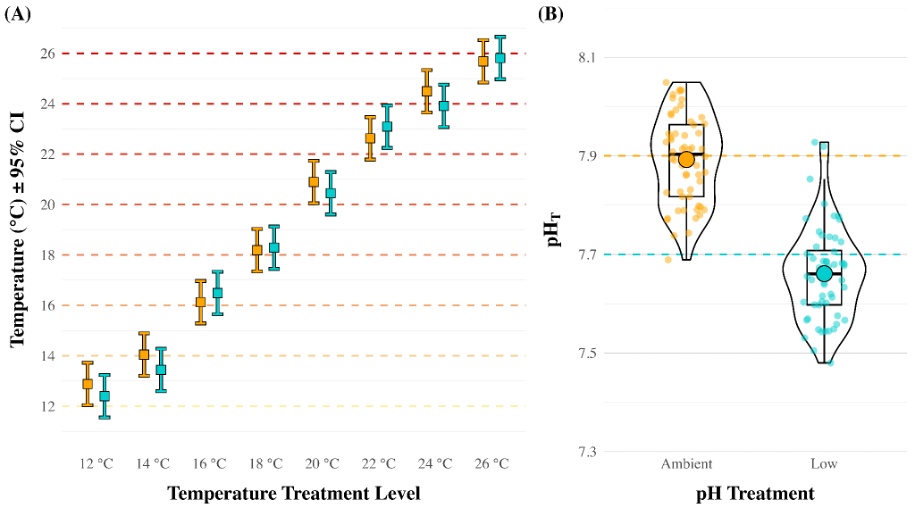
\includegraphics[width=5in]{ /Users/robertjdellinger/Documents/Github/CSUN-masters-thesis/figures/chapter2/Fig_2_3_Mesocosm_Tank_Treatments.png }
  \caption[Mesocosm mean seawater temperature and pH\textsubscript{T} across temperature and pH treatments.]{Mesocosm mean seawater temperature ($^\circ$C) and pH\textsubscript{T} between different temperature treatments (12$^\circ$C to 26$^\circ$C) and levels between ambient and low pH treatments throughout the experimental duration. (A) Mean seawater temperature ($^\circ$C) across different temperature treatments (12$^\circ$C to 26$^\circ$C) for ambient and low pH treatments throughout the experimental duration. Colored points represent mean temperatures (orange for ambient pH treatment, cyan for low pH treatment), with error bars showing 95\% confidence intervals. Horizontal dashed lines indicate set temperature treatments, color-coded from light yellow (12$^\circ$C) to dark red (26$^\circ$C). (B) Violin plot depicting the distribution of pH\textsubscript{T} values between ambient and low pH treatments. The internal boxplot within the violin plot shows the median, interquartile range, and whiskers extending to 1.5 times the interquartile range.}
  \label{fig:mesocosm_tank_treatments}
\end{figure}

\newpage

\subsection*{Elevated Respiration Rates in Response to Temperature Contrasted Between pH Levels}\label{elevated-respiration-rates-in-response-to-temperature-contrasted-between-ph-levels}
\addcontentsline{toc}{subsection}{Elevated Respiration Rates in Response to Temperature Contrasted Between pH Levels}

Respiration rates varied significantly across temperature and pH treatments, with both pH treatments having minima at approximately 12\(^\circ\)C and maxima at 24\(^\circ\)C, with higher rates generally observed under low pH conditions. For ambient pH treatment, the mean respiration rates ranged from 14.08 \(\pm\) 4.56 \(\mu\)mol O\(_2\) g\(^{-1}\) h\(^{-1}\) at 12\(^\circ\)C to 53.82 \(\pm\) 7.83 \(\mu\)mol O\(_2\) g\(^{-1}\) h\(^{-1}\) at 24\(^\circ\)C. For low pH treatment, the mean rates ranged from 11.93 \(\pm\) 0.68 \(\mu\)mol O\(_2\) g\(^{-1}\) h\(^{-1}\) at 12\(^\circ\)C to 79.47 \(\pm\) 9.21 \(\mu\)mol O\(_2\) g\(^{-1}\) h\(^{-1}\) at 24\(^\circ\)C.

\begin{figure}[H]
  \centering
  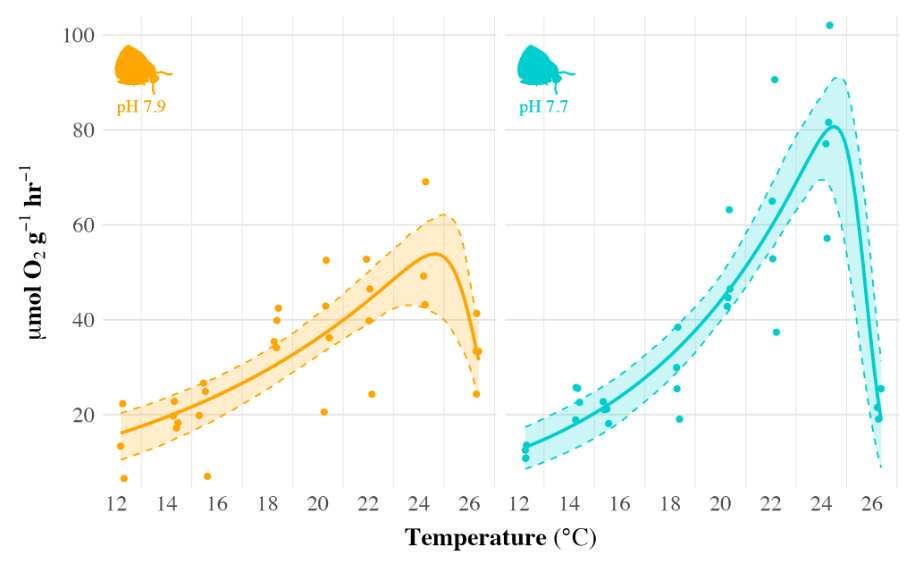
\includegraphics[width=5in]{ /Users/robertjdellinger/Documents/Github/CSUN-masters-thesis/figures/chapter2/Fig_2_4_TPC_Comparative.png }
  \caption[Comparative thermal performance curves for ambient and low pH treatments.]{Comparative thermal performance curves fitted with the Sharpe--Schoolfield high-activation model for respiration rates ($\mu$mol O$_2$ g$^{-1}$ h$^{-1}$) of *Tegula funebralis* across temperature treatments (12$^\circ$C to 26$^\circ$C) under (a) ambient and (b) low pH conditions. Solid lines represent model predictions, while shaded areas represent 95\% confidence intervals based on bootstrap analysis. Each point represents the respiration rate of an individual snail (ambient pH: $n=29$; low pH: $n=31$).}
  \label{fig:tpc_comparative}
\end{figure}

Comparative thermal performance curves revealed statistically significant differences in respiration rates (\(R_{\text{max}}\)) between ambient and low pH treatments. The \(R_{\text{max}}\) was 49.6\% higher in the low pH treatment at 80.74 \(\mu\)mol O\(_2\) g\(^{-1}\) h\(^{-1}\) (95\% CI = {[}71.85, 92.36{]}) compared to the ambient pH treatment, which had an \(R_{\text{max}}\) of 53.88 \(\mu\)mol O\(_2\) g\(^{-1}\) h\(^{-1}\) (95\% CI = {[}44.90, 62.77{]}). Other thermal performance metrics, including the optimal temperature (\(T_{\text{opt}}\)), thermal breadth (\(T_{\text{br}}\)), and critical thermal maxima (\(CT_{\text{max}}\)), were not statistically different between the pH treatments. The \(T_{\text{opt}}\) for metabolic activity was equivalent between the low pH treatment (24.49\(^\circ\)C, 95\% CI = {[}23.68, 24.88{]}) and ambient pH treatment (24.63\(^\circ\)C, 95\% CI = {[}23.30, 25.17{]}). The thermal breadth was slightly narrower in the low pH treatment (2.89, 95\% CI = {[}2.47, 3.32{]}) compared to the ambient treatment (4.26, 95\% CI = {[}3.20, 6.65{]}), suggesting a reduced range of temperatures over which organisms maintain optimal performance under low pH conditions. The \(CT_{\text{max}}\), denoting the upper thermal limit the organisms can tolerate, was found to be 27.16\(^\circ\)C (95\% CI = {[}26.70, 28.40{]}) in the low pH treatment and 28.32\(^\circ\)C (95\% CI = {[}27.40, 36.46{]}) in the ambient pH treatment. Calculations of thermal sensitivity quotients revealed the \(Q_{10}\) value was higher in the low pH treatment (2.55) compared to the ambient pH treatment (2.06), with an overall \(Q_{10}\) of 2.29.

\begin{figure}[H]
  \centering
  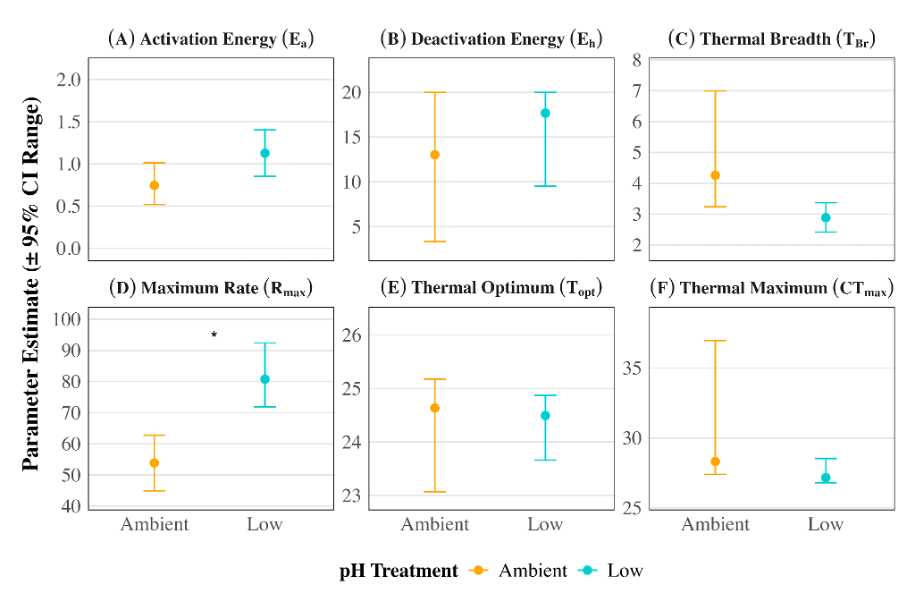
\includegraphics[width=5in]{ /Users/robertjdellinger/Documents/Github/CSUN-masters-thesis/figures/chapter2/Fig_2_5_TPC_Parameter_Estimates.png }
  \caption[Comparative thermal performance metrics between ambient and low pH treatments.]{Comparative thermal performance metrics between ambient and low pH treatments. Extracted TPC parameter estimates for the Sharpe--Schoolfield High model (high-activation) under two pH treatments (ambient and low), with accompanying bootstrapped 95\% confidence intervals. Parameters include activation energy ($E_a$), deactivation energy ($E_h$), thermal breadth ($T_{\text{br}}$), maximum rate of performance ($R_{\text{max}}$), thermal optimum ($T_{\text{opt}}$), and thermal maximum ($CT_{\text{max}}$). Points denote mean parameter estimates, vertical lines represent the 95\% bootstrapped confidence intervals, and asterisks (*) indicate significant differences between pH treatments.}
  \label{fig:tpc_metrics}
\end{figure}

\subsection*{Percent of Time Above Thermal Optimum Under Warming}\label{percent-of-time-above-thermal-optimum-under-warming}
\addcontentsline{toc}{subsection}{Percent of Time Above Thermal Optimum Under Warming}

\begin{figure}[H]
  \centering
  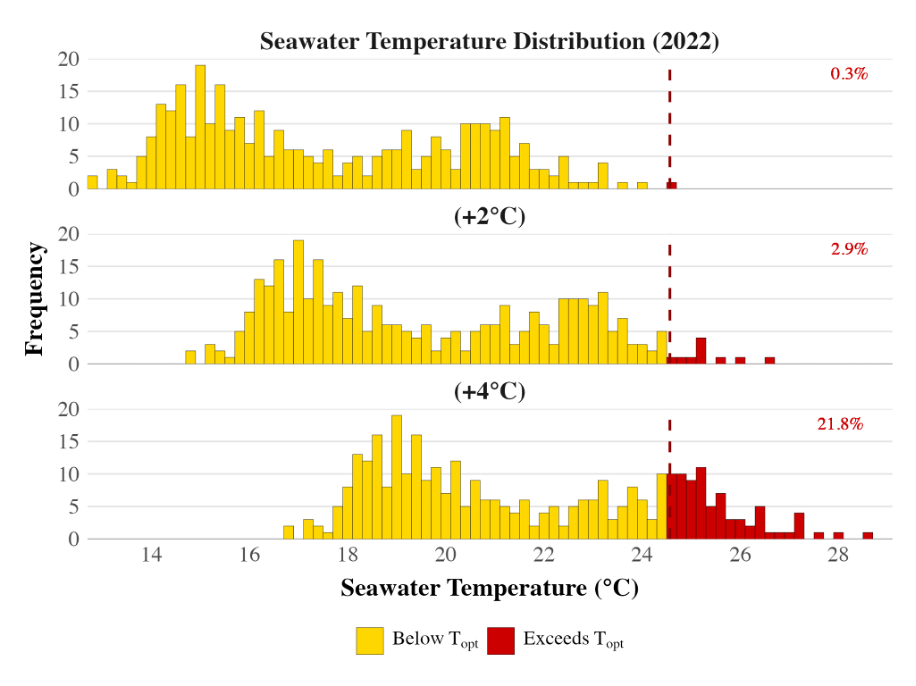
\includegraphics[width=5in]{ /Users/robertjdellinger/Documents/Github/CSUN-masters-thesis/figures/chapter2/Fig_2_6_SST_Distribution.png }
  \caption[Percent of time spent above thermal optimum under current and future warming.]{Percent of time spent above $T_{\text{opt}}$ for current and future warming predictions. Frequency distributions of daily sea surface temperatures (SST) at Newport Beach, CA—the nearest subtidal temperature station (2 meters MLLW)—under present-day conditions and hypothetical warming scenarios assuming temperature distributions remain the same (+2$^\circ$C and +4$^\circ$C). The red dashed line represents the mean SST across the observed period, while the dashed dark red line indicates the thermal optimum averaged between ambient and low pH treatments ($T_{\text{opt}} = 24.61^\circ$C) for \textit{Tegula funebralis}. Yellow bars indicate days below $T_{\text{opt}}$, and orange bars represent days exceeding $T_{\text{opt}}$.}
  \label{fig:sst_distribution}
\end{figure}

In a simple analysis of future shifts in temperature distributions, \textit{Tegula} currently experiences temperatures that exceed their \(T_{\text{opt}}\) approximately 0.29\% of the time. However, if sea surface temperatures were to rise by an additional 2\(^\circ\)C or 4\(^\circ\)C, as predicted to occur by the end of the century, the percentage of temperatures exceeding \(T_{\text{opt}}\) would increase to 2.62\% and 20.1\%, respectively.

\subsection*{Exposure to Ocean Acidification Increases Energetic Expenditure}\label{exposure-to-ocean-acidification-increases-energetic-expenditure}
\addcontentsline{toc}{subsection}{Exposure to Ocean Acidification Increases Energetic Expenditure}

\begin{figure}[H]
  \centering
  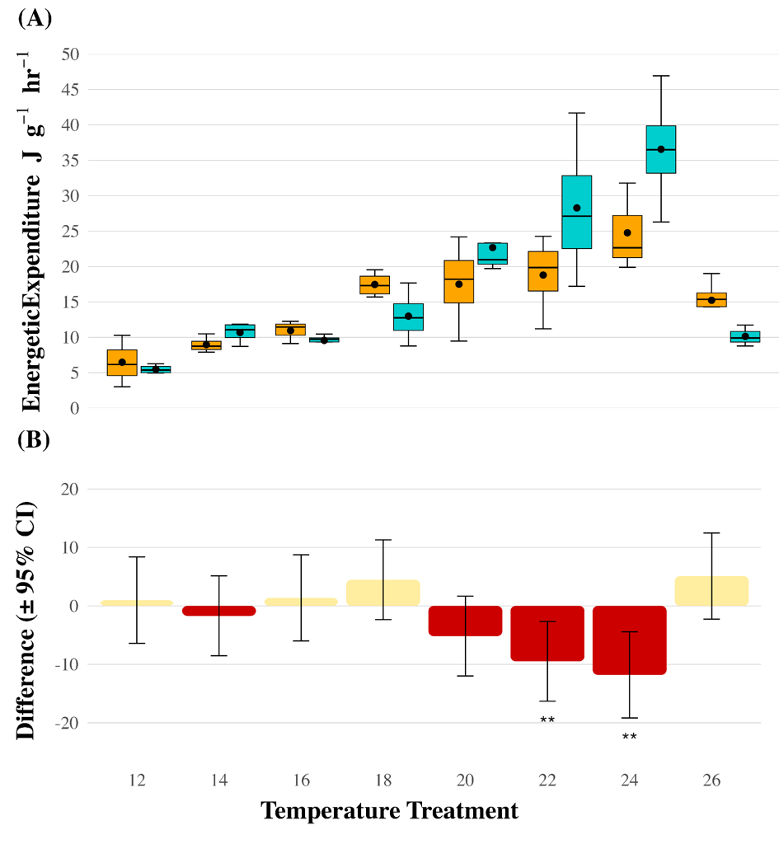
\includegraphics[width=5in]{ /Users/robertjdellinger/Documents/Github/CSUN-masters-thesis/figures/chapter2/Fig_2_7_Energetic_Expenditure.png }
  \caption[Energetic expenditure between ambient and low pH treatments.]{Energetic expenditure between ambient and low pH treatments. (A) Box plot illustrating energy expenditure (J g$^{-1}$ h$^{-1}$) across temperature treatments from 12--26$^\circ$C, colored by pH levels (ambient = orange, low = cyan). Points within the boxes represent the means, and whiskers indicate 1.5 times the interquartile range. (B) Bar plot showing pairwise differences in energetic expenditure between pH treatments at each temperature, based on Two-Way ANOVA results with $\pm$95\% confidence intervals. Red bars represent increases, and yellow bars represent decreases in energetic expenditure. Statistically significant pairwise differences, Bonferroni-adjusted, are marked with asterisks; double asterisks denote $p$-values $< 0.01$.}
  \label{fig:energetic_expenditure}
\end{figure}

A Two-Way ANOVA demonstrated a significant interaction between temperature and pH treatments on the energy requirements of \textit{Tegula funebralis} (F(7, 44) = 2.95, \(p <\) 0.05), indicating that the effect of pH on energy expenditure varied by temperature. Pairwise comparisons showed that energetic expenditure was significantly lower in the low pH treatment compared to the ambient pH treatment at both 22\(^\circ\)C (\(p <\) 0.01) and 24\(^\circ\)C (\(p <\) 0.01).

\section*{Discussion}\label{discussion}
\addcontentsline{toc}{section}{Discussion}

My findings elucidate the complex interplay between temperature and pH on organismal respiration, demonstrating that while temperature was the primary determinant of metabolic rates, ocean acidification also played a significant role in respiration rates and, thus, energetic expenditure near thermal optima. The combined effects of multiple stressors often lead to nonlinear and unpredictable outcomes, making it challenging to isolate the impact of increased energetic demands alone (Côté et al., 2016; Pörtner, 2012b; Sokolova, 2013). My findings align with ecological theories such as the Metabolic Theory of Ecology (MTE) and Oxygen- and Capacity-Limited Thermal Tolerance (OCLTT) framework, that suggest that integrating multiple aspects of global change, like ocean acidification, increases the energetic expenditure necessary to maintain physiological homeostasis and has the potential to shift physiological metrics (Brown et al., 2004; Pörtner et al., 2017).

The elevated respiration rates observed in \textit{Tegula funebralis} in response to ocean acidification in this study highlight the complex nonlinear physiological responses placed on marine organisms by multiple drivers of environmental change. The variability in metabolic rates, particularly the marked differences in the maximum metabolic rate (\(R_{\text{max}}\)) between the ambient and low pH treatments at thermal performance optima, elucidates the utility of thermal performance curves as a powerful approach for assessing multi-stressor interactions that would otherwise go uncovered. Under low pH conditions, the mean \(R_{\text{max}}\) was approximately 50\% higher than in ambient pH, illustrating a strong interaction between temperature and pH at physiological optima. These values are consistent with previous research on \textit{Tegula funebralis} (Jellison, Personal Communication; Paine, 1971), including similar species such as \textit{Littorina littorea} and \textit{Haliotis rufescens}, which have shown increased metabolic rates under acidified conditions (Michaelidis et al., 2005; Lannig et al., 2010), thus building confidence that these values are reasonable and expected.

One possible explanation for the increased metabolic rate exhibited by \textit{T. funebralis} is a compensatory response to the adverse costs of calcification induced by ocean acidification. It is plausible that the species is augmenting its metabolic rate as a means of upholding vital functions and maintaining homeostasis amidst acidic conditions. Higher aerobic respiration results in more ATP production, meeting higher energy costs associated with environmental stressors, a common compensatory mechanism observed in marine invertebrates. Additionally, the upregulation of metabolic pathways that generate ATP to meet the increased energy demands at higher temperatures, such as building calcified shell structures, compensating for changes in acid-base regulation, or contending with shell dissolution, could contribute to this increased metabolic rate (Barclay et al., 2019; Barclay et al., 2020; Brockington and Clarke, 2001; Michaelidis et al., 2005c; Swezey et al., 2020). Furthermore, higher energy demands potentially compromise the energy available for other critical biological processes such as growth, reproduction, and protein synthesis. Increased energetic demand could further impair the ability to produce heat-shock proteins and other protective measures, reducing the capacity to survive extreme temperatures (Pörtner, 2010; Stenseng et al., 2005).

Despite no significant shifts in optimal temperature (\(T_{\text{opt}}\)) or other TPC metrics across treatments, slight, but non-significant, reductions in thermal breadth (\(T_{\text{br}}\)) and increases in \(R_{\text{max}}\) under ocean acidification conditions align with our hypothesis and theoretical predictions. Moreover, there was a slight increase in activation energy (\(E_a\)), indicating higher energetic costs to maintain physiological functions in more acidic environments. These slight differences may have become clearer with a higher sample size or a longer exposure period. Additionally, the \(Q_{10}\) temperature coefficient values obtained align with Paine's (1971) value of 2.64, with a higher \(Q_{10}\) at low pH reflecting increased temperature sensitivity and demonstrating that the metabolic rate of \textit{T. funebralis} increases more rapidly with temperature in response to ocean acidification. The present study found that the respiration rate of \textit{T. funebralis} is highest between 24--25\(^\circ\)C, which is higher than other thermal performance studies of the species that have identified the thermal optimum to be around 20--22\(^\circ\)C in northern distributions of the species (Tepler et al., 2011; Tomanek and Somero, 1999). Notably, pH had the strongest impact on \textit{Tegula} energy expenditure at or near the snail's thermal optima, increasing energetic demands under more acidic conditions.

Understanding the impact of environmental changes, particularly temperature fluctuations and ocean acidification, on the organismal physiology of marine organisms is crucial for predicting their response to climate change. Previous studies have shown that \textit{T. funebralis} has a wider thermal tolerance range compared to its congeners, with a lethal temperature where 50\% of the population faces mortality (LT\(_{50}\)) at 42.5\(^\circ\)C, whereas \textit{T. brunnea} and \textit{T. montereyi}, which inhabit lower intertidal and subtidal zones, have an LT\(_{50}\) of 36\(^\circ\)C (Tomanek and Somero, 1999). Despite this broader thermal tolerance, \textit{T. funebralis} may be more vulnerable to future environmental changes, as it endures significant temperature fluctuations within the intertidal zone, often experiencing temperatures at or near its thermal limit within summer months (Stenseng et al., 2005; Tomanek and Sanford, 2003). This could mean that even subtle increases in temperature could push it beyond its physiological limits, making the species more susceptible to the anomalous events, such as marine and terrestrial heatwaves, associated with a changing climate. In a simple analysis of future shifts in temperature distributions, \textit{Tegula} currently experiences temperatures that exceed their \(T_{\text{opt}}\) approximately less than 1\% of the time. However, if sea surface temperatures were to rise by an additional 2\(^\circ\)C or 4\(^\circ\)C, as predicted to occur by the end of the century (IPCC, 2023), the percentage of temperatures exceeding \(T_{\text{opt}}\) would increase to nearly 3\% and 20\%, respectively. This suggests that future warming will substantially increase the thermal stress experienced by \textit{Tegula funebralis}, potentially impacting its survival and fitness. Coping with desiccation and heat stress requires significant energy, particularly for physiological processes like the synthesis of heat-shock proteins and maintaining cellular homeostasis in intertidal organisms such as the black turban snail, \textit{Tegula funebralis} (Tomanek, 2002; Tomanek and Somero, 2002). Increased overall energetic demand may limit \textit{Tegula}'s ability to allocate sufficient energy to these stress responses. Furthermore, increased energetic demands could impair its ability to produce heat-shock proteins and other protective measures, reducing \textit{Tegula}'s capacity to survive extreme temperatures (Pörtner, 2010; Stenseng et al., 2005). Chronic exposure to heat stress, combined with increased energetic costs, could reduce \textit{Tegula}'s long-term viability in higher intertidal zones, potentially leading to shifts in its vertical distribution.

Significant changes in energy expenditure may have profound ecological implications, potentially triggering cascading consequences for other species within intertidal ecosystems. As a generalist herbivore and detritivore species, the black turban snail consumes an array of macroalgae, microalgae, and kelp wrack (Ricketts et al., 1985; Steinberg, 1985) and their populations play a crucial role in energy transfer within intertidal ecosystems. Temperature- and ocean acidification-induced changes will affect rates of herbivory, affecting the abundance and distribution of algae, influencing the availability of space for other intertidal organisms, and altering predator-prey dynamics (Lubchenco, 1983; Yee, 2002; Nielson, 2001). This is particularly crucial as the macroalgal-herbivore interaction is the primary pathway for energy to move through trophic levels (Lubchenco and Gaines, 1981; O'Connor et al., 2009). Increased energy demands may require \textit{T. funebralis} to forage more actively and for longer periods, potentially increasing their exposure to predators and altering the algal dynamics of the ecological communities they inhabit, thereby impacting species through indirect interactions (Kroeker and Sanford, 2022; Lubchenco, 1983). Furthermore, changes in the energetic costs for \textit{Tegula}'s growth will impact both the size and structural integrity of the shells organisms produce, as evidenced by historical body size declines (Elahi et al., 2020; Barclay et al., 2019) and predator-prey experiments (Jellison and Gaylord, 2019), thereby rendering them more susceptible to predation due to alterations in optimal foraging rankings (Jellison et al., 2022; Kroeker, Sanford, et al., 2014).

Given \textit{Tegula}'s pivotal role in energy transfer and its ubiquity in intertidal ecosystems across the Pacific North American coastline, even slight changes in their energy budget could reverberate throughout the food web and indirectly impact species interactions.The annual consumption rate from a study in the Pacific Northwest was estimated at around 1,071 kcal m\(^{-2}\) yr\(^{-1}\), while the net primary production was about 1,167 kcal m\(^{-2}\) yr\(^{-1}\), with approximately 60\% of energy transferred to decomposers, illustrating \textit{Tegula}'s critical role in balancing and transferring energy throughout the ecosystem (Paine, 1971). Paine's (1969) seminal research on the keystone species concept was formulated through the \textit{Pisaster}-\textit{Tegula} interaction, illustrating how changes in the distribution of one species could cascade through the ecosystem, affecting species interactions and community structure (Paine, 1969). These impacts extend to other abundant species within intertidal ecosystems, such as \textit{Pagurus} sp. and \textit{Crepidula} sp., which utilize gastropod shells as a form of habitat specialization (Vermeij, 2020), through cooperative evolutionary strategies (Evans, 1992; Hahn, 1998; Mesce, 1993) with \textit{P. samuelis} and \textit{C. adunca} showing specific preferences for \textit{Tegula funebralis} shells. The reproductive fitness of these species is directly tied to the size, strength, and availability of these shells (Barclay et al., 2019; Gaylord et al., 2019; Taylor, 1981). Consequently, changes within one species could impact not only the biological rates and processes within its population but also extend to impacts on a network of species interactions that no theory could fully summarize.

Energetic changes induced by ocean acidification in \textit{Tegula funebralis} provide an example of broader ecological shifts. Treating concurrent changes as isolated phenomena is insufficient; embracing multiple interactions allows researchers to examine non-linear responses and determine if these interactions result in ecological surprises (Paine et al., 1998; Darling and Côté, 2008; Kroeker et al., 2017), thereby gaining better predictive power over future scenarios. As marine environments continue to warm and acidify, the metabolic costs for a wide range of species are expected to increase, leading to shifts in species distributions, species interactions, and community structure (Jellison et al., 2016; Kroeker et al., 2012; Kroeker, Sanford, et al., 2014; Pinsky et al., 2013). These changes could fundamentally disrupt the ecological balance and function of marine ecosystems. Alterations in metabolic rates of performance, such as respiration, calcification, and growth attributed to climate change, will cascade to affect net ecosystem production, net ecosystem calcification, food web dynamics, and ultimately the ecosystems humanity relies on.

\chapter*{References}\label{references}
\addcontentsline{toc}{chapter}{References}

\markboth{References}{References}

\noindent

\setlength{\parindent}{-0.20in}
\setlength{\leftskip}{0.20in}
\setlength{\parskip}{4pt}

\begingroup
\small

Akaike, H. (1974). A new look at the statistical model identification. \textit{IEEE Transactions on Automatic Control}, \textit{19}(6), 716--723. \url{https://doi.org/10.1109/TAC.1974.1100705}

\vspace{0.1em}

Allemand, D., Tambutté, É., Zoccola, D., \& Tambutté, S. (2011). Coral calcification, cells to reefs. In Z. Dubinsky \& N. Stambler (Eds.), \textit{Coral reefs: An ecosystem in transition} (pp.~119--150). Springer Netherlands. \url{https://doi.org/10.1007/978-94-007-0114-4/_9}

\vspace{0.1em}

Angilletta, M. J. (2009). \textit{Thermal adaptation: A theoretical and empirical synthesis}. Oxford University Press. \url{https://play.google.com/store/books/details?id=oN/_OxgEACAAJ}

\vspace{0.1em}

Angilletta, M. J., Jr., Huey, R. B., \& Frazier, M. R. (2010). Thermodynamic effects on organismal performance: Is hotter better? \textit{Physiological and Biochemical Zoology: PBZ}, \textit{83}(2), 197--206. \url{https://doi.org/10.1086/648567}

\vspace{0.1em}

Angilletta, M. J., Jr., Niewiarowski, P. H., \& Navas, C. A. (2002). The evolution of thermal physiology in ectotherms. \textit{Journal of Thermal Biology}, \textit{27}(4), 249--268. \url{https://doi.org/10.1016/S0306-4565(01)00094-8}

\vspace{0.1em}

Angilletta, M. J., Jr., \& Dunham, A. E. (2003). The temperature-size rule in ectotherms: Simple evolutionary explanations may not be general. \textit{The American Naturalist}, \textit{162}(3), 332--342.

\vspace{0.1em}

Arrhenius, S. (1915). Quantitative laws in biological chemistry. \textit{Nature}.

\vspace{0.1em}

Atkinson, D. (1994). Temperature and organism size---A biological law for ectotherms? \textit{Advances in Ecological Research}, \textit{25}, 1--58. \url{https://cir.nii.ac.jp/crid/1570291225611713536}

\vspace{0.1em}

Babcock, G. T., \& Wikström, M. (1992). Oxygen activation and the conservation of energy in cell respiration. \textit{Nature}, \textit{356}(6367), 301--309. \url{https://doi.org/10.1038/356301a0}

\vspace{0.1em}

Barclay, K. M., Gaylord, B., Jellison, B. M., Shukla, P., Sanford, E., \& Leighton, L. R. (2019). Variation in the effects of ocean acidification on shell growth and strength in two intertidal gastropods. \textit{Marine Ecology Progress Series}, \textit{626}, 109--121. \url{https://doi.org/10.3354/meps13056}

\vspace{0.1em}

Barclay, K. M., Gingras, M. K., Packer, S. T., \& Leighton, L. R. (2020). The role of gastropod shell composition and microstructure in resisting dissolution caused by ocean acidification. \textit{Marine Environmental Research}. \url{https://doi.org/10.1016/j.marenvres.2020.105105}

\vspace{0.1em}

Bartoń, K. (2023). MuMIn: Multi-model inference. \textit{CRAN R Project}. \url{https://cran.r-project.org/web/packages/MuMIn/index.html}

\vspace{0.1em}

Becker, D. M., \& Silbiger, N. J. (2020). Nutrient and sediment loading affect multiple facets of functionality in a tropical branching coral. \textit{The Journal of Experimental Biology}, \textit{223}(Pt 21), jeb225045. \url{https://doi.org/10.1242/jeb.225045}

\vspace{0.1em}

Bellwood, D. R., Hughes, T. P., Folke, C., \& Nyström, M. (2004). Confronting the coral reef crisis. \textit{Nature}, \textit{429}(6994), 827--833. \url{https://doi.org/10.1038/nature02691}

\vspace{0.1em}

Birk, M. A., McLean, E. L., \& Seibel, B. A. (2018). Ocean acidification does not limit squid metabolism via blood oxygen supply. \textit{The Journal of Experimental Biology}, \textit{221}(Pt 19), jeb187443. \url{https://doi.org/10.1242/jeb.187443}

\vspace{0.1em}

Boltzmann, L. (1872). \textit{Lectures on Gas Theory} (Vols. I\&II, S. G. Brush, Ed.). University of California Press.

\vspace{0.1em}

Boyd, P. W., \& Hutchins, D. A. (2012). Understanding the responses of ocean biota to a complex matrix of cumulative anthropogenic change. \textit{Marine Ecology Progress Series}, \textit{470}, 125--135. \url{https://doi.org/10.3354/meps10121}

\vspace{0.1em}

Bozinovic, F., \& Pörtner, H.-O. (2015). Physiological ecology meets climate change. \textit{Ecology and Evolution}, \textit{5}(5), 1025--1030. \url{https://doi.org/10.1002/ece3.1403}

\vspace{0.1em}

Bracken, M. E., Silbiger, N. J., Bernatchez, G., \& Sorte, C. J. (2018). Primary producers may ameliorate impacts of daytime CO\(_2\) addition in a coastal marine ecosystem. \textit{PeerJ}, \textit{6}, e4739.

\vspace{0.1em}

Brockington, S., \& Clarke, A. (2001). The relative influence of temperature and food on the metabolism of a marine invertebrate. \textit{Journal of Experimental Marine Biology and Ecology}, \textit{258}(1), 87--99. \url{https://doi.org/10.1016/S0022-0981(00)00347-6}

\vspace{0.1em}

Brown, J. H., Gillooly, J. F., Allen, A. P., Savage, V. M., \& West, G. B. (2004). Toward a metabolic theory of ecology. \textit{Ecology}, \textit{85}(7), 1771--1789. \url{https://doi.org/10.1890/03-9000}

\vspace{0.1em}

Bull, J. J. (1985). Sex ratio and nest temperature in turtles: Comparing field and laboratory data. \textit{Ecology}, \textit{66}(4), 1115--1122. \url{https://doi.org/10.2307/1939163}

\vspace{0.1em}

Burger, F. A., John, J. G., \& Frölicher, T. L. (2020). Increase in ocean acidity variability and extremes under increasing atmospheric CO\(_2\). \textit{Biogeosciences}, \textit{17}(18), 4633--4662. \url{https://doi.org/10.5194/bg-17-4633-2020}

\vspace{0.1em}

Byers, B. A., \& Mitton, J. B. (1981). Habitat choice in the intertidal snail \textit{Tegula funebralis}. \textit{Marine Biology}, \textit{65}, 149--154. \url{https://doi.org/10.1007/BF00397079}

\vspace{0.1em}

Carey, N., Harianto, J., \& Byrne, M. (2016). Sea urchins in a high-CO\(_2\) world: Partitioned effects of body size, ocean warming and acidification on metabolic rate. \textit{The Journal of Experimental Biology}, \textit{219}(Pt 8), 1178--1186. \url{https://doi.org/10.1242/jeb.136101}

\vspace{0.1em}

Carter, M. L., Flick, R. E., Terrill, E., Beckhaus, E. C., Martin, K., Fey, C. L., Walker, P. W., Largier, J. L., \& McGowan, J. A. (2023). Shore stations program, Newport Beach - Balboa Pier. In \textit{Shore stations program data archive: Current and historical coastal ocean temperature and salinity measurements from California stations}. \url{https://doi.org/10.6075/J0GX4BCP}

\vspace{0.1em}

Chavez, F. P., Ryan, J., Lluch-Cota, S. E., \& Ñiquen C, M. (2003). From anchovies to sardines and back: Multidecadal change in the Pacific Ocean. \textit{Science}, \textit{299}(5604), 217--221. \url{https://doi.org/10.1126/science.1075880}

\vspace{0.1em}

Cheng, L., Abraham, J., Trenberth, K. E., Fasullo, J., Boyer, T., Mann, M. E., Zhu, J., Wang, F., Locarnini, R., Li, Y., Zhang, B., Yu, F., Wan, L., Chen, X., Feng, L., Song, X., Liu, Y., Reseghetti, F., Simoncelli, S., \& Li, G. (2023). Another year of record heat for the oceans. \textit{Advances in Atmospheric Sciences}, \textit{40}(6), 963--974. \url{https://doi.org/10.1007/s00376-0232385-2}

\vspace{0.1em}

Clarke, A., \& Pörtner, H.-O. (2010). Temperature, metabolic power and the evolution of endothermy. \textit{Biological Reviews of the Cambridge Philosophical Society}, \textit{85}(4), 703--727. \url{https://doi.org/10.1111/j.1469-185X.2010.00122.x}

\vspace{0.1em}

Connell, J. H. (1961). The influence of interspecific competition and other factors on the distribution of the barnacle \textit{Chthamalus stellatus}. \textit{Ecology}, \textit{42}(4), 710--723. \url{https://doi.org/10.2307/1933500}

\vspace{0.1em}

Connell, J. H. (1972). Community interactions on marine rocky intertidal shores. \textit{Annual Review of Ecology and Systematics}, \textit{3}(1), 169--192. \url{https://doi.org/10.1146/annurev.es.03.110172.001125}

\vspace{0.1em}

Connell, J. H., \& Slatyer, R. O. (1977). Mechanisms of succession in natural communities and their role in community stability and organization. \textit{The American Naturalist}, \textit{111}(982), 1119--1144. \url{https://doi.org/10.1086/283241}

\vspace{0.1em}

Connolly, S. R., \& Roughgarden, J. (1998). A latitudinal gradient in northeast Pacific intertidal community structure: Evidence for an oceanographically based synthesis of marine community theory. \textit{The American Naturalist}, \textit{151}(4), 311--326. \url{https://doi.org/10.1086/286121}

\vspace{0.1em}

Cooper, E. E., \& Shanks, A. L. (2011). Latitude and coastline shape correlate with age-structure of \textit{Tegula funebralis} populations. \textit{Marine Ecology Progress Series}, \textit{424}, 133--143. \url{https://doi.org/10.3354/meps08993}

\vspace{0.1em}

Corris, A. (2020). Defining the environment in organism--environment systems. \textit{Frontiers in Psychology}, \textit{11}, 1285. \url{https://doi.org/10.3389/fpsyg.2020.01285}

\vspace{0.1em}

Côté, I. M., Darling, E. S., \& Brown, C. J. (2016). Interactions among ecosystem stressors and their importance in conservation. \textit{Proceedings of the Royal Society B}, \textit{283}(1824), 20152592. \url{https://doi.org/10.1098/rspb.2015.2592}

\vspace{0.1em}

Darling, E. S., \& Côté, I. M. (2008). Quantifying the evidence for ecological synergies. \textit{Ecology Letters}, \textit{11}(12), 1278--1286. \url{https://doi.org/10.1111/j.1461-0248.2008.01243.x}

\vspace{0.1em}

Davis, J. L. D. (2001). Diel changes in habitat use by two tidepool fishes. \textit{Copeia}, \textit{2001}(3), 835--841. \url{https://doi.org/10.1643/0045-8511(2001)001\%5B0835:DCIHUB\%5D2.0.CO;2}

\vspace{0.1em}

Dayton, P. K. (1971). Competition, disturbance, and community organization: The provision and subsequent utilization of space in a rocky intertidal community. \textit{Ecological Monographs}, \textit{41}(4), 351--389. \url{https://doi.org/10.2307/1948498}

\vspace{0.1em}

Dell, A. I., Pawar, S., \& Savage, V. M. (2011). Systematic variation in the temperature dependence of physiological and ecological traits. \textit{Proceedings of the National Academy of Sciences of the United States of America}, \textit{108}(26), 10591--10596. \url{https://doi.org/10.1073/pnas.1015178108}

\vspace{0.1em}

Denny, M., \& Wethey, D. (2001). Physical processes that generate patterns in marine communities. In \textit{Marine Community Ecology} (pp.~3--37).

\vspace{0.1em}

Deser, C., Alexander, M. A., Xie, S.-P., \& Phillips, A. S. (2010). Sea surface temperature variability: Patterns and mechanisms. \textit{Annual Review of Marine Science}, \textit{2}, 115--143. \url{https://doi.org/10.1146/annurev-marine-120408-151453}

\vspace{0.1em}

Dickson, A. G., Sabine, C. L., \& Christian, J. R. (2007). \textit{Guide to Best Practices for Ocean CO$_2$ Measurements}. PICES Special Publication.

\vspace{0.1em}

Doney, S. C., Fabry, V. J., Feely, R. A., \& Kleypas, J. A. (2009). Ocean acidification: The other CO\(_2\) problem. \textit{Annual Review of Marine Science}, \textit{1}, 169--192. \url{https://doi.org/10.1146/annurev.marine.010908.163834}

\vspace{0.1em}

Dowd, W. W., King, F. A., \& Denny, M. W. (2015). Thermal variation, thermal extremes and the physiological performance of individuals. \textit{The Journal of Experimental Biology}, \textit{218}(Pt 12), 1956--1967. \url{https://doi.org/10.1242/jeb.114926}

\vspace{0.1em}

Edmunds, P. J., \& Davies, P. S. (1986). An energy budget for \textit{Porites porites} (Scleractinia). \textit{Marine Biology}, \textit{92}, 339--347. \url{https://doi.org/10.1007/BF00392674}

\vspace{0.1em}

Elahi, R., Miller, L. P., \& Litvin, S. Y. (2020). Historical comparisons of body size are sensitive to data availability and ecological context. \textit{Ecology}, \textit{101}(9), e03101. \url{https://doi.org/10.1002/ecy.3101}

\vspace{0.1em}

Elliott, J. M., \& Davison, W. (1975). Energy equivalents of oxygen consumption in animal energetics. \textit{Oecologia}, \textit{19}(3), 195--201. \url{https://doi.org/10.1007/BF00345305}

\vspace{0.1em}

Erlandson, J. M., Ainis, A. F., Braje, T. J., Jew, N. P., McVey, M., Rick, T. C., Vellanoweth, R. L., \& Watts, J. (2015). 12,000 years of human predation on black turban snails (\textit{Chlorostoma funebralis}) on Alta California's Northern Channel Islands. \textit{California Archaeology}, \textit{7}(1), 59--91. \url{https://doi.org/10.1179/1947461X15Z.00000000056}

\vspace{0.1em}

Erlandson, J. M., Graham, M. H., Bourque, B. J., Corbett, D., Estes, J. A., \& Steneck, R. S. (2007). The Kelp Highway Hypothesis: Marine ecology, the coastal migration theory, and the peopling of the Americas. \textit{The Journal of Island and Coastal Archaeology}, \textit{2}(2), 161--174. \url{https://doi.org/10.1080/15564890701628612}

\vspace{0.1em}

Estes, J. A., \& Palmisano, J. F. (1974). Sea otters: Their role in structuring nearshore communities. \textit{Science}, \textit{185}(4156), 1058--1060. \url{https://doi.org/10.1126/science.185.4156.1058}

\vspace{0.1em}

Evans, S. M. (1992). Comparative studies of two epizoic limpets, \textit{Collisella asmi} and \textit{Crepidula adunca}, on shells of turban snails (\textit{Tegula} spp.). \textit{Marine Behaviour and Physiology}, \textit{19}(4), 241--249. \url{https://doi.org/10.1080/10236249209378812}

\vspace{0.1em}

Fawcett, M. H. (1984). Local and latitudinal variation in predation on an herbivorous marine snail. \textit{Ecology}, \textit{65}(4), 1214--1230. \url{https://doi.org/10.2307/1938329}

\vspace{0.1em}

Feely, R. A., Sabine, C. L., Byrne, R. H., Millero, F. J., Dickson, A. G., Wanninkhof, R., Murata, A., Miller, L. A., \& Greeley, D. (2012). Decadal changes in the aragonite and calcite saturation state of the Pacific Ocean. \textit{Global Biogeochemical Cycles}, \textit{26}(3). \url{https://doi.org/10.1029/2011GB004157}

\vspace{0.1em}

Feely, R. A., Sabine, C. L., Hernandez-Ayon, J. M., Ianson, D., \& Hales, B. (2008). Evidence for upwelling of corrosive ``acidified'' water onto the continental shelf. \textit{Science}, \textit{320}(5882), 1490--1492. \url{https://doi.org/10.1126/science.1155676}

\vspace{0.1em}

Feely, R. A., Sabine, C. L., Lee, K., Berelson, W., Kleypas, J., Fabry, V. J., \& Millero, F. J. (2004). Impact of anthropogenic CO\(_2\) on the CaCO\(_3\) system in the oceans. \textit{Science}, \textit{305}(5682), 362--366. \url{https://doi.org/10.1126/science.1097329}

\vspace{0.1em}

Fields, J. B., \& Silbiger, N. J. (2022). Foundation species loss alters multiple ecosystem functions within temperate tidepool communities. \textit{Marine Ecology Progress Series}, \textit{679}, 1--18. \url{https://doi.org/10.3354/meps13978}

\vspace{0.1em}

Fox, J., \& Weisberg, S. (2018). \textit{An R Companion to Applied Regression} (3rd ed.). SAGE Publications. \url{https://play.google.com/store/books/details?id=uPNrDwAAQBAJ}

\vspace{0.1em}

Frank, P. W. (1975). Latitudinal variation in the life history features of the black turban snail \textit{Tegula funebralis} (Prosobranchia: Trochidae). \textit{Marine Biology}, \textit{31}(2), 181--192. \url{https://doi.org/10.1007/BF00391630}

\vspace{0.1em}

Friedlingstein, P., O'Sullivan, M., Jones, M. W., Andrew, R. M., Gregor, L., Hauck, J., Le Quéré, C., Luijkx, I. T., Olsen, A., \& Peters, G. P. (2022). Global carbon budget 2022. \textit{Earth System Science Data}, \textit{14}(11), 4811--4900. \url{https://doi.org/10.5194/essd-14-4811-2022}

\vspace{0.1em}

Gammon, M., Fossette, S., McGrath, G., \& Mitchell, N. (2020). A systematic review of metabolic heat in sea turtle nests and methods to model its impact on hatching success. \textit{Frontiers in Ecology and Evolution}, \textit{8}, 556379. \url{https://doi.org/10.3389/fevo.2020.556379}

\vspace{0.1em}

García-Reyes, M., \& Largier, J. L. (2012). Seasonality of coastal upwelling off central and northern California: New insights, including temporal and spatial variability. \textit{Journal of Geophysical Research: Oceans}, \textit{117}(C3). \url{https://doi.org/10.1029/2011JC007629}

\vspace{0.1em}

Gattuso, J.-P., Epitalon, J.-M., Lavigne, H., Orr, J., Gentili, B., Hagens, M., Hofmann, A., Mueller, J.-D., Proye, A., Rae, J., \& Others. (2015). \textit{seacarb: Seawater carbonate chemistry with R}. R package version 3.2.12.

\vspace{0.1em}

Gaylord, B., Barclay, K. M., Jellison, B. M., Jurgens, L. J., Ninokawa, A. T., Rivest, E. B., \& Leighton, L. R. (2019). Ocean change within shoreline communities: From biomechanics to behaviour and beyond. \textit{Conservation Physiology}, \textit{7}(1), coz077. \url{https://doi.org/10.1093/conphys/coz077}

\vspace{0.1em}

Gaylord, B., Kroeker, K. J., Sunday, J. M., Anderson, K. M., Barry, J. P., Brown, N. E., Connell, S. D., Dupont, S., Fabricius, K. E., Hall-Spencer, J. H., Klinger, T., Milazzo, M., Munday, P. L., Russell, B. D., Sanford, E., Schreiber, S. J., Thiyagarajan, V., Vaughan, M. L. H., Widdicombe, S., \& Harley, C. D. G. (2015). Ocean acidification through the lens of ecological theory. \textit{Ecology}, \textit{96}(1), 3--15. \url{https://doi.org/10.1890/14-0802.1}

\vspace{0.1em}

Gazeau, F., Quiblier, C., Jansen, J. M., Gattuso, J.-P., Middelburg, J. J., \& Heip, C. H. R. (2007). Impact of elevated CO\(_2\) on shellfish calcification. \textit{Geophysical Research Letters}, \textit{34}(7). \url{https://doi.org/10.1029/2006GL028554}

\vspace{0.1em}

Erlandson, J. M., Ainis, A. F., Braje, T. J., Jew, N. P., McVey, M., Rick, T. C., Vellanoweth, R. L., \& Watts, J. (2015). 12,000 years of human predation on black turban snails (\textit{Chlorostoma funebralis}) on Alta California's Northern Channel Islands. \textit{California Archaeology}, \textit{7}(1), 59--91. \url{https://doi.org/10.1179/1947461X15Z.00000000056}

\vspace{0.1em}

Erlandson, J. M., Graham, M. H., Bourque, B. J., Corbett, D., Estes, J. A., \& Steneck, R. S. (2007). The Kelp Highway Hypothesis: Marine ecology, the coastal migration theory, and the peopling of the Americas. \textit{The Journal of Island and Coastal Archaeology}, \textit{2}(2), 161--174. \url{https://doi.org/10.1080/15564890701628612}

\vspace{0.1em}

Estes, J. A., \& Palmisano, J. F. (1974). Sea otters: Their role in structuring nearshore communities. \textit{Science}, \textit{185}(4156), 1058--1060. \url{https://doi.org/10.1126/science.185.4156.1058}

\vspace{0.1em}

Evans, S. M. (1992). Comparative studies of two epizoic limpets, \textit{Collisella asmi} and \textit{Crepidula adunca}, on shells of turban snails (\textit{Tegula} spp.). \textit{Marine Behaviour and Physiology}, \textit{19}(4), 241--249. \url{https://doi.org/10.1080/10236249209378812}

\vspace{0.1em}

Fawcett, M. H. (1984). Local and latitudinal variation in predation on an herbivorous marine snail. \textit{Ecology}, \textit{65}(4), 1214--1230. \url{https://doi.org/10.2307/1938329}

\vspace{0.1em}

Feely, R. A., Sabine, C. L., Byrne, R. H., Millero, F. J., Dickson, A. G., Wanninkhof, R., Murata, A., Miller, L. A., \& Greeley, D. (2012). Decadal changes in the aragonite and calcite saturation state of the Pacific Ocean. \textit{Global Biogeochemical Cycles}, \textit{26}(3). \url{https://doi.org/10.1029/2011GB004157}

\vspace{0.1em}

Feely, R. A., Sabine, C. L., Hernandez-Ayon, J. M., Ianson, D., \& Hales, B. (2008). Evidence for upwelling of corrosive ``acidified'' water onto the continental shelf. \textit{Science}, \textit{320}(5882), 1490--1492. \url{https://doi.org/10.1126/science.1155676}

\vspace{0.1em}

Feely, R. A., Sabine, C. L., Lee, K., Berelson, W., Kleypas, J., Fabry, V. J., \& Millero, F. J. (2004). Impact of anthropogenic CO\(_2\) on the CaCO\(_3\) system in the oceans. \textit{Science}, \textit{305}(5682), 362--366. \url{https://doi.org/10.1126/science.1097329}

\vspace{0.1em}

Fields, J. B., \& Silbiger, N. J. (2022). Foundation species loss alters multiple ecosystem functions within temperate tidepool communities. \textit{Marine Ecology Progress Series}, \textit{679}, 1--18. \url{https://doi.org/10.3354/meps13978}

\vspace{0.1em}

Fox, J., \& Weisberg, S. (2018). \textit{An R Companion to Applied Regression} (3rd ed.). SAGE Publications. \url{https://play.google.com/store/books/details?id=uPNrDwAAQBAJ}

\vspace{0.1em}

Frank, P. W. (1975). Latitudinal variation in the life history features of the black turban snail \textit{Tegula funebralis} (Prosobranchia: Trochidae). \textit{Marine Biology}, \textit{31}(2), 181--192. \url{https://doi.org/10.1007/BF00391630}

\vspace{0.1em}

Friedlingstein, P., O'Sullivan, M., Jones, M. W., Andrew, R. M., Gregor, L., Hauck, J., Le Quéré, C., Luijkx, I. T., Olsen, A., \& Peters, G. P. (2022). Global carbon budget 2022. \textit{Earth System Science Data}, \textit{14}(11), 4811--4900. \url{https://doi.org/10.5194/essd-14-4811-2022}

\vspace{0.1em}

Gammon, M., Fossette, S., McGrath, G., \& Mitchell, N. (2020). A systematic review of metabolic heat in sea turtle nests and methods to model its impact on hatching success. \textit{Frontiers in Ecology and Evolution}, \textit{8}, 556379. \url{https://doi.org/10.3389/fevo.2020.556379}

\vspace{0.1em}

García-Reyes, M., \& Largier, J. L. (2012). Seasonality of coastal upwelling off central and northern California: New insights, including temporal and spatial variability. \textit{Journal of Geophysical Research: Oceans}, \textit{117}(C3). \url{https://doi.org/10.1029/2011JC007629}

\vspace{0.1em}

Gattuso, J.-P., Epitalon, J.-M., Lavigne, H., Orr, J., Gentili, B., Hagens, M., Hofmann, A., Mueller, J.-D., Proye, A., Rae, J., \& Others. (2015). \textit{seacarb: Seawater carbonate chemistry with R}. R package version 3.2.12.

\vspace{0.1em}

Gaylord, B., Barclay, K. M., Jellison, B. M., Jurgens, L. J., Ninokawa, A. T., Rivest, E. B., \& Leighton, L. R. (2019). Ocean change within shoreline communities: From biomechanics to behaviour and beyond. \textit{Conservation Physiology}, \textit{7}(1), coz077. \url{https://doi.org/10.1093/conphys/coz077}

\vspace{0.1em}

Gaylord, B., Kroeker, K. J., Sunday, J. M., Anderson, K. M., Barry, J. P., Brown, N. E., Connell, S. D., Dupont, S., Fabricius, K. E., Hall-Spencer, J. H., Klinger, T., Milazzo, M., Munday, P. L., Russell, B. D., Sanford, E., Schreiber, S. J., Thiyagarajan, V., Vaughan, M. L. H., Widdicombe, S., \& Harley, C. D. G. (2015). Ocean acidification through the lens of ecological theory. \textit{Ecology}, \textit{96}(1), 3--15. \url{https://doi.org/10.1890/14-0802.1}

\vspace{0.1em}

Gazeau, F., Quiblier, C., Jansen, J. M., Gattuso, J.-P., Middelburg, J. J., \& Heip, C. H. R. (2007). Impact of elevated CO\(_2\) on shellfish calcification. \textit{Geophysical Research Letters}, \textit{34}(7). \url{https://doi.org/10.1029/2006GL028554}

\vspace{0.1em}

\vspace{0.1em}

Hijmans, R. J., Van Etten, J., Cheng, J., Mattiuzzi, M., Sumner, M., Greenberg, J. A., Lamigueiro, O. P., Bevan, A., Racine, E. B., Shortridge, A., \& others. (2015). \textit{raster: Geographic Data Analysis and Modeling} (R package version 2.5-2). \url{https://cran.r-project.org/package=raster}

\vspace{0.1em}

Hochachka, P. W. (1967). Organization of metabolism during temperature compensation. In M. F. Prosser (Ed.), \textit{Molecular Mechanisms of Temperature Adaptation} (pp.~177--203). American Elsevier.

\vspace{0.1em}

Hochachka, P. W., \& Somero, G. N. (2002). \textit{Biochemical adaptation: Mechanism and process in physiological evolution}. Oxford University Press.

\vspace{0.1em}

Hoegh-Guldberg, O., Mumby, P. J., Hooten, A. J., Steneck, R. S., Greenfield, P., Gomez, E., Harvell, C. D., Sale, P. F., Edwards, A. J., Caldeira, K., Knowlton, N., Eakin, C. M., Iglesias-Prieto, R., Muthiga, N., Bradbury, R. H., Dubi, A., \& Hatziolos, M. E. (2007). Coral reefs under rapid climate change and ocean acidification. \textit{Science}, \textit{318}(5857), 1737--1742. \url{https://doi.org/10.1126/science.1152509}

\vspace{0.1em}

Hofmann, G. E., Evans, T. G., Kelly, M. W., Padilla-Gamiño, J. L., Blanchette, C. A., Washburn, L., Chan, F., McManus, M. A., Menge, B. A., \& Gaylord, B. (2014). Exploring local adaptation and the ocean acidification seascape---studies in the California Current Large Marine Ecosystem. \textit{Biogeosciences}, \textit{11}(4), 1053--1064. \url{https://doi.org/10.5194/bg-11-1053-2014}

\vspace{0.1em}

Hofmann, G. E., \& Todgham, A. E. (2010). Living in the now: Physiological mechanisms to tolerate a rapidly changing environment. \textit{Annual Review of Physiology}, \textit{72}, 127--145. \url{https://doi.org/10.1146/annurev-physiol-021909-135900}

\vspace{0.1em}

Huey, R. B., \& Kingsolver, J. G. (1989). Evolution of thermal sensitivity of ectotherm performance. \textit{Trends in Ecology \& Evolution}, \textit{4}(5), 131--135. \url{https://doi.org/10.1016/0169-5347(89)90211-5}

\vspace{0.1em}

Huey, R. B., \& Stevenson, R. D. (1979). Integrating thermal physiology and ecology of ectotherms: A discussion of approaches. \textit{American Zoologist}, \textit{19}(1), 357--366. \url{https://doi.org/10.1093/icb/19.1.357}

\vspace{0.1em}

IPCC. (2023). \textit{Climate Change 2023: Synthesis Report}. Contribution of Working Groups I, II and III to the Sixth Assessment Report of the Intergovernmental Panel on Climate Change (H. Lee, J. Skea, P. Zhai, D. Roberts, P. R. Shukla, A. Mukherjee, E. C. Buendia, \& K. Tanabe, Eds.). IPCC. \url{https://doi.org/10.59327/IPCC/AR6-9789291691647}

\vspace{0.1em}

Jellison, B. M., \& Gaylord, B. (2019). Shifts in seawater chemistry disrupt trophic links within a simple shoreline food web. \textit{Oecologia}, \textit{190}(4), 955--967. \url{https://doi.org/10.1007/s00442-019-04422-9}

\vspace{0.1em}

Jellison, B. M., Elsmore, K. E., Miller, J. T., Ng, G., Ninokawa, A. T., Hill, T. M., \& Gaylord, B. (2022). Low-pH seawater alters indirect interactions in rocky-shore tidepools. \textit{Ecology and Evolution}, \textit{12}(2), e8607. \url{https://doi.org/10.1002/ece3.8607}

\vspace{0.1em}

Jellison, B. M., Ninokawa, A. T., Hill, T. M., Sanford, E., \& Gaylord, B. (2016). Ocean acidification alters the response of intertidal snails to a key sea star predator. \textit{Proceedings of the Royal Society B: Biological Sciences}, \textit{283}(1833), 20160890. \url{https://doi.org/10.1098/rspb.2016.0890}

\vspace{0.1em}

Jones, E., \& Long, J. D. (2018). Geographic variation in the sensitivity of an herbivore-induced seaweed defense. \textit{Ecology}, \textit{99}(8), 1748--1758. \url{https://doi.org/10.1002/ecy.2407}

\vspace{0.1em}

Katz, M. E., Finkel, Z. V., Grzebyk, D., Knoll, A. H., \& Falkowski, P. G. (2004). Evolutionary trajectories and biogeochemical impacts of marine eukaryotic phytoplankton. \textit{Annual Review of Ecology, Evolution, and Systematics}, \textit{35}, 523--556. \url{https://doi.org/10.1146/annurev.ecolsys.35.112202.130137}

\vspace{0.1em}

Kahle, D., \& Wickham, H. (2013). ggmap: Spatial visualization with ggplot2. \textit{The R Journal}, \textit{5}(1), 144--161. \url{https://doi.org/10.32614/RJ-2013-014}

\vspace{0.1em}

Kingsolver, J. G., \& Huey, R. B. (2008). Size, temperature, and fitness: Three rules. \textit{Evolutionary Ecology Research}, \textit{10}(2), 251--268.

\vspace{0.1em}

Kordas, R. L., Harley, C. D. G., \& O'Connor, M. I. (2011). Community ecology in a warming world: The influence of temperature on interspecific interactions in marine systems. \textit{Journal of Experimental Marine Biology and Ecology}, \textit{400}(1--2), 218--226. \url{https://doi.org/10.1016/j.jembe.2011.02.029}

\vspace{0.1em}

Kroeker, K. J., Gambi, M. C., \& Micheli, F. (2013). Community dynamics and ecosystem simplification in a high-CO\(_2\) ocean. \textit{Proceedings of the National Academy of Sciences}, \textit{110}(31), 12721--12726. \url{https://doi.org/10.1073/pnas.1216464110}

\vspace{0.1em}

Kroeker, K. J., Gaylord, B., Hill, T. M., Hosfelt, J. D., Miller, S. H., \& Sanford, E. (2014). The role of temperature in determining species' vulnerability to ocean acidification: A case study using \textit{Mytilus galloprovincialis}. \textit{PLoS ONE}, \textit{9}(7), e100353. \url{https://doi.org/10.1371/journal.pone.0100353}

\vspace{0.1em}

Kroeker, K. J., Kordas, R. L., Crim, R., Hendriks, I. E., Ramajo, L., Singh, G. S., Duarte, C. M., \& Gattuso, J.-P. (2013). Impacts of ocean acidification on marine organisms: Quantifying sensitivities and interaction with warming. \textit{Global Change Biology}, \textit{19}(6), 1884--1896. \url{https://doi.org/10.1111/gcb.12179}

\vspace{0.1em}

Kroeker, K. J., Kordas, R. L., \& Harley, C. D. G. (2017). Embracing interactions in ocean acidification research: Confronting multiple stressor scenarios and context dependence. \textit{Biology Letters}, \textit{13}(3), 20160802. \url{https://doi.org/10.1098/rsbl.2016.0802}

\vspace{0.1em}

Kroeker, K. J., Micheli, F., \& Gambi, M. C. (2012). Ocean acidification causes ecosystem shifts via altered competitive interactions. \textit{Nature Climate Change}, \textit{3}(2), 156--159. \url{https://doi.org/10.1038/nclimate1680}

\vspace{0.1em}

Kroeker, K. J., \& Sanford, E. (2022). Ecological leverage points: Species interactions amplify the physiological effects of global environmental change in the ocean. \textit{Annual Review of Marine Science}, \textit{14}, 75--103. \url{https://doi.org/10.1146/annurev-marine-042021-051211}

\vspace{0.1em}

Kroeker, K. J., Sanford, E., Jellison, B. M., \& Gaylord, B. (2014). Predicting the effects of ocean acidification on predator-prey interactions: A conceptual framework based on coastal molluscs. \textit{The Biological Bulletin}, \textit{226}(3), 211--222. \url{https://doi.org/10.1086/BBLv226n3p211}

\vspace{0.1em}

Kroeker, K. J., Sanford, E., Rose, J. M., Blanchette, C. A., Chan, F., Chavez, F. P., Gaylord, B., Helmuth, B., Hill, T. M., Hofmann, G. E., McManus, M. A., Menge, B. A., Nielsen, K. J., Raimondi, P. T., Russell, A. D., \& Washburn, L. (2016). Interacting environmental mosaics drive geographic variation in mussel performance and predation vulnerability. \textit{Ecology Letters}, \textit{19}(7), 771--779. \url{https://doi.org/10.1111/ele.12613}

\vspace{0.1em}

Kunze, C., Wölfelschneider, M., \& Rölfer, L. (2021). Multiple driver impacts on rocky intertidal systems: The need for an integrated approach. \textit{Frontiers in Marine Science}, \textit{8}, 667168. \url{https://doi.org/10.3389/fmars.2021.667168}

\vspace{0.1em}

Kwiatkowski, L., Gaylord, B., Hill, T. M., Hosfelt, J., Kroeker, K. J., Nebuchina, Y., Ninokawa, A., Russell, A. D., Rivest, E. B., \& Sesboüé, M. (2016). Nighttime dissolution in a temperate coastal ocean ecosystem increases under acidification. \textit{Scientific Reports}, \textit{6}(1), 22984. \url{https://doi.org/10.1038/srep22984}

\vspace{0.1em}

Lefevre, S. (2016). Are global warming and ocean acidification conspiring against marine ectotherms? A meta-analysis of the respiratory effects of elevated temperature, high CO\(_2\), and their interaction. \textit{Conservation Physiology}, \textit{4}(1), cow009. \url{https://doi.org/10.1093/conphys/cow009}

\vspace{0.1em}

Lenth, R. V. (2016). Least-squares means: The R package \texttt{lsmeans}. \textit{Journal of Statistical Software}, \textit{69}, 1--33. \url{https://doi.org/10.18637/jss.v069.i01}

\vspace{0.1em}

Levene, H. (1961). Robust tests for equality of variances. In I. Olkin (Ed.), \textit{Contributions to Probability and Statistics} (pp.~278--292). Stanford University Press.

\vspace{0.1em}

Levin, S. A., \& Paine, R. T. (1974). Disturbance, patch formation, and community structure. \textit{Proceedings of the National Academy of Sciences}, \textit{71}(7), 2744--2747. \url{https://doi.org/10.1073/pnas.71.7.2744}

\vspace{0.1em}

Levin, S. A. (1992). The problem of pattern and scale in ecology: The Robert H. MacArthur award lecture. \textit{Ecology}, \textit{73}(6), 1943--1967. \url{https://doi.org/10.2307/1941447}

\vspace{0.1em}

Levins, R. (1968). \textit{Evolution in changing environments}. Princeton University Press.

\vspace{0.1em}

Levins, R. (1969). Thermal acclimation and heat resistance in \textit{Drosophila} species. \textit{The American Naturalist}, \textit{103}(933), 483--499. \url{https://doi.org/10.1086/282616}

\vspace{0.1em}

Levins, R., \& Lewontin, R. (1985). \textit{The dialectical biologist}. Harvard University Press.

\vspace{0.1em}

Lewontin, R. (1983). The organism as the subject and object of evolution. \textit{Scientia; Rivista Di Scienza}, \textit{77}(18).

\vspace{0.1em}

Licker, R., Ekwurzel, B., Doney, S. C., Cooley, S. R., Lima, I. D., Heede, R., \& Frumhoff, P. C. (2019). Attributing ocean acidification to major carbon producers. \textit{Environmental Research Letters}, \textit{14}(12), 124060. \url{https://doi.org/10.1088/1748-9326/ab5e6b}

\vspace{0.1em}

Luan, L., Jiang, Y., Dini-Andreote, F., Crowther, T. W., Li, P., Bahram, M., Zheng, J., Xu, Q., Zhang, X.-X., \& Sun, B. (2023). Integrating pH into the metabolic theory of ecology to predict bacterial diversity in soil. \textit{Proceedings of the National Academy of Sciences of the United States of America}, \textit{120}(3), e2207832120. \url{https://doi.org/10.1073/pnas.2207832120}

\vspace{0.1em}

Lubchenco, J. (1978). Plant species diversity in a marine intertidal community: Importance of herbivore food preference and algal competitive abilities. \textit{The American Naturalist}, \textit{112}(983), 23--39. \url{https://doi.org/10.1086/283250}

\vspace{0.1em}

Lubchenco, J. (1983). \textit{Littorina} and \textit{Fucus}: Effects of herbivores, substratum heterogeneity, and plant escapes during succession. \textit{Ecology}, \textit{64}(5), 1116--1123. \url{https://doi.org/10.2307/1937822}

\vspace{0.1em}

Lubchenco, J., \& Gaines, S. D. (1981). A unified approach to marine plant-herbivore interactions. I. Populations and communities. \textit{Annual Review of Ecology and Systematics}, \textit{12}, 405--437. \url{https://doi.org/10.1146/annurev.es.12.110181.002201}

\vspace{0.1em}

Lüdecke, D., Ben-Shachar, M. S., Patil, I., Waggoner, P., \& Makowski, D. (2021). \texttt{performance}: An R package for assessment, comparison and testing of statistical models. \textit{Journal of Open Source Software}, \textit{6}(60), 3139. \url{https://doi.org/10.21105/joss.03139}

\vspace{0.1em}

Mekkes, L., Renema, W., Bednaršek, N., Alin, S. R., Feely, R. A., Huisman, J., Roessingh, P., \& Peijnenburg, K. T. C. A. (2021). Pteropods make thinner shells in the upwelling region of the California Current ecosystem. \textit{Scientific Reports}, \textit{11}(1), 1731. \url{https://doi.org/10.1038/s41598-021-81131-9}

\vspace{0.1em}

Menge, B. A., \& Sutherland, J. P. (1987). Community regulation: Variation in disturbance, competition, and predation in relation to environmental stress and recruitment. \textit{The American Naturalist}, \textit{130}(5), 730--757. \url{https://doi.org/10.1086/284741}

\vspace{0.1em}

Mesce, K. A. (1993). The shell selection behavior of two closely related hermit crabs. \textit{Animal Behaviour}, \textit{45}(4), 659--671. \url{https://doi.org/10.1006/anbe.1993.1081}

\vspace{0.1em}

Michaelidis, B., Ouzounis, C., Paleras, A., \& Pörtner, H. O. (2005a). Effects of long-term moderate hypercapnia on acid--base balance and growth rate in marine mussels \textit{Mytilus galloprovincialis}. \textit{Marine Ecology Progress Series}, \textit{293}, 109--118. \url{https://doi.org/10.3354/meps293109}

\vspace{0.1em}

Michaelidis, B., Ouzounis, C., Paleras, A., \& Pörtner, H. O. (2005b). Effects of long-term moderate hypercapnia on acid--base balance and growth rate in marine mussels \textit{Mytilus galloprovincialis}. \textit{Marine Ecology Progress Series}, \textit{293}, 109--118. \url{https://doi.org/10.3354/meps293109}

\vspace{0.1em}

Michaelidis, B., Ouzounis, C., Paleras, A., \& Pörtner, H. O. (2005c). Effects of long-term moderate hypercapnia on acid--base balance and growth rate in marine mussels \textit{Mytilus galloprovincialis}. \textit{Marine Ecology Progress Series}, \textit{293}, 109--118. \url{https://doi.org/10.3354/meps293109}

\vspace{0.1em}

\vspace{0.1em}

Moré, J. J. (1978). The Levenberg--Marquardt algorithm: Implementation and theory. In G. A. Watson (Ed.), \textit{Numerical Analysis: Proceedings of the Dundee Conference on Numerical Analysis} (pp.~105--116). Springer. \url{https://doi.org/10.1007/BFb0067700}

\vspace{0.1em}

Morris, R. H., Abbott, D. P., \& Haderlie, E. C. (1980). \textit{Intertidal invertebrates of California}. Stanford University Press.

\vspace{0.1em}

Multi-Agency Rocky Intertidal Network (MARINe), Partnership for Interdisciplinary Studies of Coastal Oceans (PISCO), \& Burnaford, J. (2023). MARINe/PISCO: Intertidal: Site temperature data: Point Fermin, California (IPTFXX) {[}dataset{]}. \url{https://doi.org/10.6085/AA/IPTFXX/_XXXITV2XMSR01/_20220130.50.1}

\vspace{0.1em}

Munday, P. L., Dixson, D. L., Donelson, J. M., Jones, G. P., Pratchett, M. S., Devitsina, G. V., \& Døving, K. B. (2009). Ocean acidification impairs olfactory discrimination and homing ability of a marine fish. \textit{Proceedings of the National Academy of Sciences}, \textit{106}(6), 1848--1852. \url{https://doi.org/10.1073/pnas.0809996106}

\vspace{0.1em}

Mundim, K. C., Baraldi, S., Machado, H. G., \& Vieira, F. M. C. (2020). Temperature coefficient (Q\(_{10}\)) and its applications in biological systems: Beyond the Arrhenius theory. \textit{Ecological Modelling}, \textit{431}, 109127. \url{https://doi.org/10.1016/j.ecolmodel.2020.109127}

\vspace{0.1em}

Nielsen, K. J. (2001). Bottom-up and top-down forces in tide pools: Test of a food chain model in an intertidal community. \textit{Ecological Monographs}, \textit{71}(2), 187--206. \url{https://doi.org/10.1890/0012-9615(2001)071\%5B0187:BUATDF\%5D2.0.CO;2}

\vspace{0.1em}

O'Connor, M. I., Bruno, J. F., Gaines, S. D., Halpern, B. S., Lester, S. E., Kinlan, B. P., \& Weiss, J. M. (2007). Temperature control of larval dispersal and the implications for marine ecology, evolution, and conservation. \textit{Proceedings of the National Academy of Sciences}, \textit{104}(4), 1266--1271. \url{https://doi.org/10.1073/pnas.0603422104}

\vspace{0.1em}

O'Connor, M. I., Piehler, M. F., Leech, D. M., Anton, A., \& Bruno, J. F. (2009). Warming and resource availability shift food web structure and metabolism. \textit{PLOS Biology}, \textit{7}(8), e1000178. \url{https://doi.org/10.1371/journal.pbio.1000178}

\vspace{0.1em}

Odum, E. P. (1968). Energy flow in ecosystems: A historical review. \textit{American Zoologist}, \textit{8}(1), 11--18. \url{https://doi.org/10.1093/icb/8.1.11}

\vspace{0.1em}

Olito, C., White, C. R., Marshall, D. J., \& Barneche, D. R. (2017). Estimating monotonic rates from biological data using local linear regression. \textit{The Journal of Experimental Biology}, \textit{220}(5), 759--764. \url{https://doi.org/10.1242/jeb.148775}

\vspace{0.1em}

Orr, J. C., Fabry, V. J., Aumont, O., Bopp, L., Doney, S. C., Feely, R. A., Gnanadesikan, A., Gruber, N., Ishida, A., \& Joos, F. (2005). Anthropogenic ocean acidification over the twenty-first century and its impact on calcifying organisms. \textit{Nature}, \textit{437}(7059), 681--686. \url{https://doi.org/10.1038/nature04095}

\vspace{0.1em}

\vspace{0.1em}

Pacific Rocky Intertidal Monitoring. (2004). Pacific rocky intertidal monitoring: Long-term monitoring of rocky intertidal communities. University of California, Santa Cruz. Retrieved June 7, 2024, from \url{https://rockyintertidal.cisr.ucsc.edu/}

\vspace{0.1em}

Padfield, D., \& Matheson, G. (2023). nls.multstart: Robust non-linear regression using AIC scores {[}R package{]}. \url{https://cran.r-project.org/package=nls.multstart}

\vspace{0.1em}

Padfield, D., O'Sullivan, H., \& Pawar, S. (2021). rTPC and nls.multstart: A new pipeline to fit thermal performance curves in R. \textit{Methods in Ecology and Evolution}, \textit{12}(7), 1138--1143. \url{https://doi.org/10.1111/2041-210X.13585}

\vspace{0.1em}

Paine, R. T. (1966). Food web complexity and species diversity. \textit{The American Naturalist}, \textit{100}(910), 65--75. \url{https://doi.org/10.1086/282400}

\vspace{0.1em}

Paine, R. T. (1969). The Pisaster--Tegula interaction: Prey patches, predator food preference, and intertidal community structure. \textit{Ecology}, \textit{50}(6), 950--961. \url{https://doi.org/10.2307/1936888}

\vspace{0.1em}

Paine, R. T. (1971). Energy flow in a population of the herbivorous gastropod \textit{Tegula funebralis}. \textit{Limnology and Oceanography}, \textit{16}(1), 86--98. \url{https://doi.org/10.4319/lo.1971.16.1.0086}

\vspace{0.1em}

Paine, R. T. (1980). Food webs: Linkage, interaction strength and community infrastructure. \textit{The Journal of Animal Ecology}, \textit{49}(3), 667--685. \url{https://doi.org/10.2307/4220}

\vspace{0.1em}

Paine, R. T., \& Gould, C. E. (1977). Controlled manipulations in the marine intertidal zone and their contributions to ecological theory. \textit{Proceedings of the Academy of Natural Sciences of Philadelphia}, \textit{128}, 245--270.

\vspace{0.1em}

Paine, R. T., Tegner, M. J., \& Johnson, E. A. (1998). Compounded perturbations yield ecological surprises. \textit{Ecosystems}, \textit{1}(6), 535--545. \url{https://doi.org/10.1007/s100219900049}

\vspace{0.1em}

Patil, I. (2021). Visualizations with statistical details: The ``ggstatsplot'' approach. \textit{Journal of Open Source Software}, \textit{6}(61), 3167. \url{https://doi.org/10.21105/joss.03167}

\vspace{0.1em}

Pebesma, E. (2018). Simple features for R: Standardized support for spatial vector data. \textit{The R Journal}, \textit{10}(1), 439--446. \url{https://doi.org/10.32614/RJ-2018-009}

\vspace{0.1em}

Pinsky, M. L., Worm, B., Fogarty, M. J., Sarmiento, J. L., \& Levin, S. A. (2013). Marine taxa track local climate velocities. \textit{Science}, \textit{341}(6151), 1239--1242. \url{https://doi.org/10.1126/science.1239352}

\vspace{0.1em}

Poloczanska, E. S., Burrows, M. T., Brown, C. J., Molinos, J. G., Halpern, B. S., Hoegh-Guldberg, O., Kappel, C. V., Moore, P. J., Richardson, A. J., Schoeman, D. S., \& Sydeman, W. J. (2016). Responses of marine organisms to climate change across oceans. \textit{Frontiers in Marine Science}, \textit{3}, 62. \url{https://doi.org/10.3389/fmars.2016.00062}

\vspace{0.1em}

\vspace{0.1em}

Pörtner, H.-O. (2010). Oxygen- and capacity-limitation of thermal tolerance: a matrix for integrating climate-related stressor effects in marine ecosystems. \textit{The Journal of Experimental Biology}, \textit{213}(6), 881--893. \url{https://doi.org/10.1242/jeb.037523}

\vspace{0.1em}

Pörtner, H. O. (2012a). Integrating climate-related stressor effects on marine organisms: unifying principles linking molecule to ecosystem-level changes. \textit{Marine Ecology Progress Series}, \textit{470}, 273--290. \url{https://doi.org/10.3354/meps10123}

\vspace{0.1em}

Pörtner, H. O. (2012b). Integrating climate-related stressor effects on marine organisms: unifying principles linking molecule to ecosystem-level changes. \textit{Marine Ecology Progress Series}, \textit{470}, 273--290. \url{https://doi.org/10.3354/meps10123}

\vspace{0.1em}

Pörtner, H.-O., Bock, C., \& Mark, F. C. (2017). Oxygen- and capacity-limited thermal tolerance: bridging ecology and physiology. \textit{The Journal of Experimental Biology}, \textit{220}(Pt 15), 2685--2696. \url{https://doi.org/10.1242/jeb.134585}

\vspace{0.1em}

Pörtner, H. O., \& Farrell, A. P. (2008). Physiology and climate change. \textit{Science}, \textit{322}(5902), 690--692. \url{https://doi.org/10.1126/science.1163156}

\vspace{0.1em}

Pörtner, H. O., \& Knust, R. (2007). Climate change affects marine fishes through the oxygen limitation of thermal tolerance. \textit{Science}, \textit{315}(5808), 95--97. \url{https://doi.org/10.1126/science.1135471}

\vspace{0.1em}

Raffaelli, D. G., \& Hawkins, S. J. (1996). \textit{Intertidal Ecology}. Springer Science \& Business Media.

\vspace{0.1em}

Rasmussen, L. L., Carter, M. L., Flick, R. E., Hilbern, M., Fumo, J. T., Cornuelle, B. D., Gordon, B. K., Bargatze, L. F., Gordon, R. L., \& McGowan, J. A. (2020). A century of southern California coastal ocean temperature measurements. \textit{Journal of Geophysical Research: Oceans}, \textit{125}(5), e2019JC015673. \url{https://doi.org/10.1029/2019JC015673}

\vspace{0.1em}

R Core Team. (2023). \textit{R: A Language and Environment for Statistical Computing}. R Foundation for Statistical Computing. \url{https://www.R-project.org/}

\vspace{0.1em}

Ricketts, E. F., Calvin, J., Hedgpeth, J. W., \& Phillips, D. W. (1985). \textit{Between Pacific Tides} (5th ed.). Stanford University Press. \url{https://play.google.com/store/books/details?id=tUl5ESavtRIC}

\vspace{0.1em}

Ries, J. B., Cohen, A. L., \& McCorkle, D. C. (2009). Marine calcifiers exhibit mixed responses to CO\(_2\)-induced ocean acidification. \textit{Geology}, \textit{37}(12), 1131--1134. \url{https://doi.org/10.1130/G30210A.1}

\vspace{0.1em}

\vspace{0.1em}

Sanford, E. (1999). Regulation of keystone predation by small changes in ocean temperature. \textit{Science}, \textit{283}(5410), 2095--2097. \url{https://doi.org/10.1126/science.283.5410.2095}

\vspace{0.1em}

Schmidt-Nielsen, K. (1997). \textit{Animal Physiology: Adaptation and Environment} (5th ed.). Cambridge University Press. \url{https://play.google.com/store/books/details?id=Af7IwQWJoCMC}

\vspace{0.1em}

Schoolfield, R. M., Sharpe, P. J., \& Magnuson, C. E. (1981). Non-linear regression of biological temperature-dependent rate models based on absolute reaction-rate theory. \textit{Journal of Theoretical Biology}, \textit{88}(4), 719--731. \url{https://doi.org/10.1016/0022-5193(81)90246-0}

\vspace{0.1em}

Schulte, P. M. (2015). The effects of temperature on aerobic metabolism: towards a mechanistic understanding of the responses of ectotherms to a changing environment. \textit{The Journal of Experimental Biology}, \textit{218}(12), 1856--1866. \url{https://doi.org/10.1242/jeb.118851}

\vspace{0.1em}

Schulte, P. M., Healy, T. M., \& Fangue, N. A. (2011). Thermal performance curves, phenotypic plasticity, and the time scales of temperature exposure. \textit{Integrative and Comparative Biology}, \textit{51}(5), 691--702. \url{https://doi.org/10.1093/icb/icr097}

\vspace{0.1em}

Seebacher, F., White, C. R., \& Franklin, C. E. (2015). Physiological plasticity increases resilience of ectothermic animals to climate change. \textit{Nature Climate Change}, \textit{5}(1), 61--66. \url{https://doi.org/10.1038/nclimate2457}

\vspace{0.1em}

Shapiro, S. S., \& Wilk, M. B. (1965). An analysis of variance test for normality (complete samples). \textit{Biometrika}, \textit{52}(3--4), 591--611. \url{https://doi.org/10.1093/biomet/52.3-4.591}

\vspace{0.1em}

Sharpe, P. J., \& DeMichele, D. W. (1977). Reaction kinetics of poikilotherm development. \textit{Journal of Theoretical Biology}, \textit{64}(4), 649--670. \url{https://doi.org/10.1016/0022-5193(77)90265-x}

\vspace{0.1em}

Sharpley, C. F., \& Koehn, C. (2022). Frequency and content of the last fifty years of papers on Aristotle's writings on biological phenomena. \textit{Journal of the History of Biology}, \textit{55}(3), 585--607. \url{https://doi.org/10.1007/s10739-022-09683-8}

\vspace{0.1em}

Silbiger, N. J., Donahue, M. J., \& Lubarsky, K. (2020). Submarine groundwater discharge alters coral reef ecosystem metabolism. \textit{Proceedings of the Royal Society B}, \textit{287}(1941), 20202743. \url{https://doi.org/10.1098/rspb.2020.2743}

\vspace{0.1em}

Silbiger, N. J., Goodbody-Gringley, G., Bruno, J. F., \& Putnam, H. M. (2019). Comparative thermal performance of the reef-building coral \textit{Orbicella franksi} at its latitudinal range limits. \textit{Marine Biology}, \textit{166}(10), 1--14. \url{https://doi.org/10.1007/s00227-019-3573-6}

\vspace{0.1em}

Silbiger, N. J., \& Sorte, C. J. B. (2018). Biophysical feedbacks mediate carbonate chemistry in coastal ecosystems across spatiotemporal gradients. \textit{Scientific Reports}, \textit{8}(1), 796. \url{https://doi.org/10.1038/s41598-017-18736-6}

\vspace{0.1em}

\vspace{0.1em}

Sinclair, B. J., Marshall, K. E., Sewell, M. A., Levesque, D. L., Willett, C. S., Slotsbo, S., Dong, Y., Harley, C. D. G., Marshall, D. J., Helmuth, B. S., \& Huey, R. B. (2016). Can we predict ectotherm responses to climate change using thermal performance curves and body temperatures? \textit{Ecology Letters}, \textit{19}(11), 1372--1385. \url{https://doi.org/10.1111/ele.12686}

\vspace{0.1em}

Sjoberg, D. D., Whiting, K., Curry, M., Lavery, J. A., \& Larmarange, J. (2021). Reproducible summary tables with the gtsummary package. \textit{The R Journal}, \textit{13}(1), 570--580. \url{https://doi.org/10.32614/RJ-2021-053}

\vspace{0.1em}

Sokolova, I. M. (2013). Energy-limited tolerance to stress as a conceptual framework to integrate the effects of multiple stressors. \textit{Integrative and Comparative Biology}, \textit{53}(4), 597--608. \url{https://doi.org/10.1093/icb/ict028}

\vspace{0.1em}

Somero, G. N. (1995). Proteins and temperature. \textit{Annual Review of Physiology}, \textit{57}(1), 43--68. \url{https://doi.org/10.1146/annurev.physiol.57.030195.000355}

\vspace{0.1em}

Somero, G. N. (2002). Thermal physiology and vertical zonation of intertidal animals: optima, limits, and costs of living. \textit{Integrative and Comparative Biology}, \textit{42}(4), 780--789. \url{https://doi.org/10.1093/icb/42.4.780}

\vspace{0.1em}

Somero, G. N. (2011). Comparative physiology: a ``crystal ball'' for predicting consequences of global change. \textit{American Journal of Physiology-Regulatory, Integrative and Comparative Physiology}, \textit{301}(1), R1--R14. \url{https://doi.org/10.1152/ajpregu.00719.2010}

\vspace{0.1em}

Somero, G. N. (2020). The cellular stress response and temperature: Function, regulation, and evolution. \textit{Journal of Experimental Zoology Part A: Ecological and Integrative Physiology}, \textit{333}(6), 379--397. \url{https://doi.org/10.1002/jez.2344}

\vspace{0.1em}

Somero, G. N. (2022). Solutions: How adaptive changes in cellular fluids enable marine life to cope with abiotic stressors. \textit{Marine Life Science \& Technology}, \textit{4}(3), 389--413. \url{https://doi.org/10.1007/s42995-022-00140-3}

\vspace{0.1em}

Somero, G. N., Beers, J. M., Chan, F., Hill, T. M., Klinger, T., \& Litvin, S. Y. (2016). What changes in the carbonate system, oxygen, and temperature portend for the northeastern Pacific Ocean: A physiological perspective. \textit{Bioscience}, \textit{66}(1), 14--26. \url{https://doi.org/10.1093/biosci/biv162}

\vspace{0.1em}

Sorte, C. J. B., Bernatchez, G., Mislan, K. A. S., Pandori, L. L. M., Silbiger, N. J., \& Wallingford, P. D. (2019). Thermal tolerance limits as indicators of current and future intertidal zonation patterns in a diverse mussel guild. \textit{Marine Biology}, \textit{166}(1), 1--13. \url{https://doi.org/10.1007/s00227-018-3452-6}

\vspace{0.1em}

Spalding, C., Finnegan, S., \& Fischer, W. W. (2017). Energetic costs of calcification under ocean acidification. \textit{Global Biogeochemical Cycles}, \textit{31}(5), 866--877. \url{https://doi.org/10.1002/2016GB005597}

\vspace{0.1em}

Steinberg, P. D. (1985). Feeding preferences of \textit{Tegula funebralis} and chemical defenses of marine brown algae. \textit{Ecological Monographs}, \textit{55}(3), 333--349. \url{https://doi.org/10.2307/1942581}

\vspace{0.1em}

\vspace{0.1em}

Stenseng, E., Braby, C. E., \& Somero, G. N. (2005). Evolutionary and acclimation-induced variation in the thermal limits of heart function in congeneric marine snails (\textit{genus Tegula}): Implications for vertical zonation. \textit{The Biological Bulletin}, \textit{208}(2), 138--144. \url{https://doi.org/10.2307/3593122}

\vspace{0.1em}

Stenseth, N. C., Mysterud, A., Ottersen, G., Hurrell, J. W., Chan, K.-S., \& Lima, M. (2002). Ecological effects of climate fluctuations. \textit{Science}, \textit{297}(5585), 1292--1296. \url{https://doi.org/10.1126/science.1071281}

\vspace{0.1em}

Suster, C. (2023). \textit{ggmapinset}: Add inset panels to maps. \url{https://cran.r-project.org/package=ggmapinset}

\vspace{0.1em}

Swezey, D. S., Boles, S. E., Aquilino, K. M., Stott, H. K., Bush, D., Whitehead, A., Rogers-Bennett, L., Hill, T. M., \& Sanford, E. (2020). Evolved differences in energy metabolism and growth dictate the impacts of ocean acidification on abalone aquaculture. \textit{Proceedings of the National Academy of Sciences of the United States of America}, \textit{117}(42), 26513--26519. \url{https://doi.org/10.1073/pnas.2006910117}

\vspace{0.1em}

Sydeman, W. J., García-Reyes, M., Schoeman, D. S., Rykaczewski, R. R., Thompson, S. A., Black, B. A., \& Bograd, S. J. (2014). Climate change and wind intensification in coastal upwelling ecosystems. \textit{Science}, \textit{345}(6192), 77--80. \url{https://doi.org/10.1126/science.1251635}

\vspace{0.1em}

Taylor, A. R., Brownlee, C., \& Wheeler, G. L. (2012). Proton channels in algae: Reasons to be excited. \textit{Trends in Plant Science}, \textit{17}(11), 675--684. \url{https://doi.org/10.1016/j.tplants.2012.06.009}

\vspace{0.1em}

Taylor, P. R. (1981). Hermit crab fitness: The effect of shell condition and behavioral adaptations on environmental resistance. \textit{Journal of Experimental Marine Biology and Ecology}, \textit{52}(2), 205--218. \url{https://doi.org/10.1016/0022-0981(81)90037-X}

\vspace{0.1em}

Tepler, S., Mach, K., \& Denny, M. (2011). Preference versus performance: Body temperature of the intertidal snail \textit{Chlorostoma funebralis}. \textit{The Biological Bulletin}, \textit{220}(2), 107--117. \url{https://doi.org/10.1086/BBLv220n2p107}

\vspace{0.1em}

Todgham, A. E., Schulte, P. M., \& Iwama, G. K. (2005). Cross-tolerance in the tidepool sculpin: The role of heat shock proteins. \textit{Physiological and Biochemical Zoology: PBZ}, \textit{78}(2), 133--144. \url{https://doi.org/10.1086/425205}

\vspace{0.1em}

Todgham, A. E., \& Stillman, J. H. (2013). Physiological responses to shifts in multiple environmental stressors: Relevance in a changing world. \textit{Integrative and Comparative Biology}, \textit{53}(4), 539--544. \url{https://doi.org/10.1093/icb/ict086}

\vspace{0.1em}

Tomanek, L. (2002). The heat-shock response: Its variation, regulation and ecological importance in intertidal gastropods (\textit{genus Tegula}). \textit{Integrative and Comparative Biology}, \textit{42}(4), 797--807. \url{https://doi.org/10.1093/icb/42.4.797}

\vspace{0.1em}

Tomanek, L., \& Helmuth, B. (2002). Physiological ecology of rocky intertidal organisms: A synergy of concepts. \textit{Integrative and Comparative Biology}, \textit{42}(4), 771--775. \url{https://doi.org/10.1093/icb/42.4.771}

\vspace{0.1em}

Tomanek, L., \& Sanford, E. (2003). Heat-shock protein 70 (Hsp70) as a biochemical stress indicator: An experimental field test in two congeneric intertidal gastropods (\textit{genus Tegula}). \textit{The Biological Bulletin}, \textit{205}(3), 276--284. \url{https://doi.org/10.2307/1543291}

\vspace{0.1em}

Tomanek, L., \& Somero, G. N. (1999). Evolutionary and acclimation-induced variation in the heat-shock responses of congeneric marine snails (\textit{genus Tegula}) from different thermal habitats: Implications for limits of thermotolerance and biogeography. \textit{The Journal of Experimental Biology}, \textit{202}(Pt 21), 2925--2936. \url{https://doi.org/10.1242/jeb.202.21.2925}

\vspace{0.1em}

Tomanek, L., \& Somero, G. N. (2002). Interspecific- and acclimation-induced variation in levels of heat-shock proteins 70 (HSP70) and 90 (HSP90) and heat-shock transcription factor-1 (HSF1) in congeneric marine snails (\textit{genus Tegula}): Implications for regulation of hsp gene expression. \textit{The Journal of Experimental Biology}, \textit{205}(Pt 5), 677--685. \url{https://doi.org/10.1242/jeb.205.5.677}

\vspace{0.1em}

Toniello, G., Lepofsky, D., Lertzman-Lepofsky, G., Salomon, A. K., \& Rowell, K. (2019). 11,500 years of human--clam relationships provide long-term context for intertidal management in the Salish Sea, British Columbia. \textit{Proceedings of the National Academy of Sciences}, \textit{116}(44), 22106--22114. \url{https://doi.org/10.1073/pnas.1905921116}

\vspace{0.1em}

Vermeij, G. J. (2020). Choice and the evolution of habitat specialization: The case of life on shells. \textit{Marine Biology}, \textit{167}(7), 94. \url{https://doi.org/10.1007/s00227-020-03710-0}

\vspace{0.1em}

Von Bertalanffy, L. (1957). Quantitative laws in metabolism and growth. \textit{The Quarterly Review of Biology}, \textit{32}(3), 217--231. \url{https://doi.org/10.1086/401873}

\vspace{0.1em}

Welch, B. L. (1947). The generalization of ``Student's'' problem when several different population variances are involved. \textit{Biometrika}, \textit{34}(1/2), 28--35. \url{https://doi.org/10.2307/2332510}

\vspace{0.1em}

Whiteley, N. M. (2011). Physiological and ecological responses of crustaceans to ocean acidification. \textit{Marine Ecology Progress Series}, \textit{430}, 257--271. \url{https://doi.org/10.3354/meps09185}

\vspace{0.1em}

Wolfe, K., Nguyen, H. D., Davey, M., \& Byrne, M. (2020). Characterizing biogeochemical fluctuations in a world of extremes: A synthesis for temperate intertidal habitats in the face of global change. \textit{Global Change Biology}, \textit{26}(7), 3858--3879. \url{https://doi.org/10.1111/gcb.15103}

\vspace{0.1em}

Wolfe, W. H., Martz, T. R., Dickson, A. G., Goericke, R., \& Ohman, M. D. (2023). A 37-year record of ocean acidification in the southern California current. \textit{Communications Earth \& Environment}, \textit{4}(1), 406. \url{https://doi.org/10.1038/s43247-023-01065-0}

\vspace{0.1em}

Wolff, N. H., Donner, S. D., Cao, L., Iglesias-Prieto, R., Sale, P. F., \& Mumby, P. J. (2015). Global inequities between polluters and the polluted: Climate change impacts on coral reefs. \textit{Global Change Biology}, \textit{21}(11), 3982--3994. \url{https://doi.org/10.1111/gcb.13015}

\vspace{0.1em}

Woodwell, G. M. (1970). Effects of pollution on the structure and physiology of ecosystems: Changes in natural ecosystems caused by many different types of disturbances are similar and predictable. \textit{Science}, \textit{168}(3930), 429--433. \url{https://doi.org/10.1126/science.168.3930.429}

\vspace{0.1em}

Yee, E. H. (2002). Effects of temperature on activity, food consumption rates, and gut passage times of three seaweed-eating species of \textit{Tegula} (Trochidae) from central and southern California (Master's thesis, California State University, Fullerton).

\begingroup
\normalsize

\appendix

\chapter*{Appendix A: Supplemental Figures}\label{appendix-a-supplemental-figures}
\addcontentsline{toc}{chapter}{Appendix A: Supplemental Figures}

\addcontentsline{toc}{chapter}{Appendix A: Supplemental Figures}
\setcounter{figure}{0}
\renewcommand{\thefigure}{A\arabic{figure}}

\begin{figure}[H]
\centering
\caption[Histogram plots of seawater temperature and pH$_\mathrm{T}$.]{Histogram plots of daily average seawater temperature (°C) and pH$_\mathrm{T}$ measurements from a continuous subtidal monitoring station illustrating coastal ocean variability. (A) Distribution of daily average seawater temperature from a subtidal monitoring station at Newport Beach Pier, depicting observed frequencies from 2020 to 2024, with dashed horizontal lines representing the set temperature treatments of the experiment, and the labeled mean for the temperature distribution ($\hat{\mu}$). (B) Distribution of daily average pH$_\mathrm{T}$ measurements at Newport Beach Pier, depicting observed frequencies from 2020–2024, with vertical dashed lines indicating the set pH treatment values of the experiment and a labeled mean of the pH$_\mathrm{T}$ distribution ($\hat{\mu}$). Temperature and pH data were filtered to exclude flagged and extreme values, followed by a calculation of daily averages. Histogram plots were created using the \texttt{ggstatsplot} package in R (Patil, 2021). Data for these plots were provided by the Southern California Coastal Ocean Observing System and the Shore Stations Program at the Scripps Institution of Oceanography, supported by the California Department of Parks and Recreation, Natural Resources Division, Award\#C1670003 (Carter et al., 2023).}
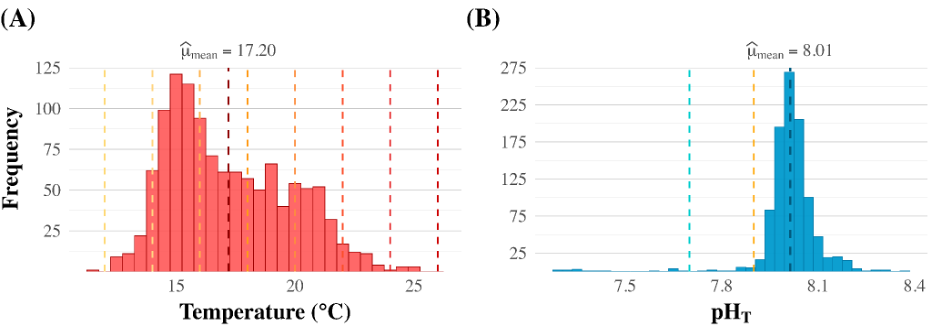
\includegraphics[width=5in]{figures/appendix/Appendix_1_SST_pH.png}
\label{fig:appendixA1}
\end{figure}

\chapter*{Appendix B: Supplemental Tables}\label{appendix-b-supplemental-tables}
\addcontentsline{toc}{chapter}{Appendix B: Supplemental Tables}

\addcontentsline{toc}{chapter}{Appendix B: Supplemental Tables}
\setcounter{table}{0}
\renewcommand{\thetable}{B\arabic{table}}

\begin{table}[H]
\caption[Summary statistics for mesocosm tank treatments.]{Summary statistics table (Mean ± SE) for tank treatments and associated water quality and biogeochemistry parameters subjected to low and ambient pH levels alongside temperature variations ranging from 12–26$^\circ$C. The depicted parameters include temperature ($^\circ$C), pH$_\mathrm{T}$ (total scale), salinity (ppt), dissolved oxygen (mg L$^{-1}$), total alkalinity (TA), partial pressure of CO$_2$ ($p$CO$_2$), mean bicarbonate concentration (HCO$_3^-$), carbonate concentration (CO$_3^{2-}$), and dissolved inorganic carbon (DIC) computed using the \texttt{seacarb} package in R (Gattuso et al., 2015). Summary table created using the \texttt{gtsummary} package (Sjoberg et al., 2021).}
\centering
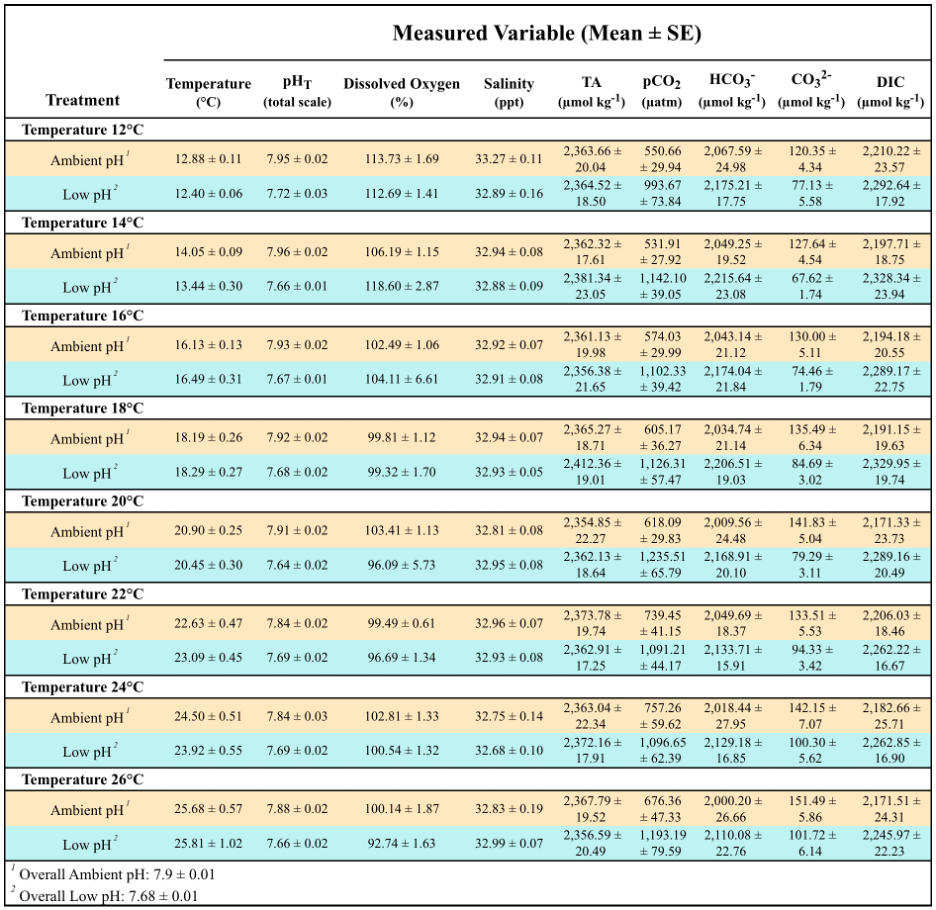
\includegraphics[width=5.5in]{figures/appendix/Appendix_2_Mesocosm_Table.png}
\label{tab:appendixB1}
\end{table}

\begin{table}[H]
\caption[Welch's $t$-test results for pH differences.]{Welch's $t$-Test for difference of pH between pH treatment groups. Results display group means ($\bar{x}$), difference in means ($\bar{x}_{\text{ambient}} - \bar{x}_{\text{low}}$), 95\% confidence intervals (CI), degrees of freedom (df), $t$-statistic, and $p$-value.}
\centering
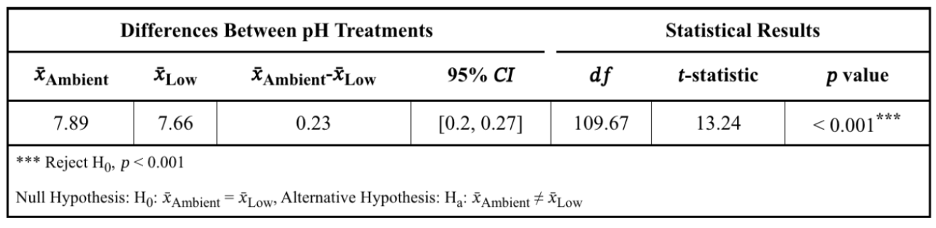
\includegraphics[width=6in]{figures/appendix/Appendix_3_ttest_pH.png}
\label{tab:appendixB2}
\end{table}

\newpage

\begin{table}[H]
\caption[Two-Way ANOVA for seawater temperature treatments.]{Two-Way ANOVA results for temperature ($^\circ$C) by temperature treatment and pH treatment to test for significant differences in seawater conditions between tanks. ANOVA results include main effects of Temperature Treatment, pH treatment, and their interaction as sources of variation, with degrees of freedom (df), sum of squares (SS), mean squares (MS), $F$-Statistic, and $p$-value.}
\centering
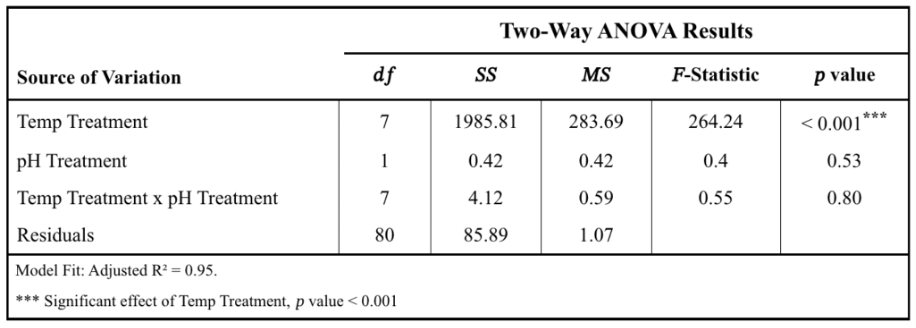
\includegraphics[width=5in]{figures/appendix/Appendix_4_Mesocosm_ANOVA_Temp.png}
\label{tab:appendixB3}
\end{table}

\newpage

\begin{table}[H]
\caption[Comparative model fits for respiration rates.]{Comparative model fits and fitted curve plots for respiration rates ($\mu$mol O$_2$ g$^{-1}$ h$^{-1}$) across temperature (12–26$^\circ$C) between low and ambient pH treatments, based on Sharpe-Schoolfield (High-Activation) model estimates. Best-fit models were selected by lowest corrected AICc value. Bootstrap analysis summary table presents coefficient estimates, standard errors ($\sigma_{\bar{x}}$), p-values, and biases for both pH treatments. Significant coefficients ($p < 0.001$) are marked with asterisks.}
\centering
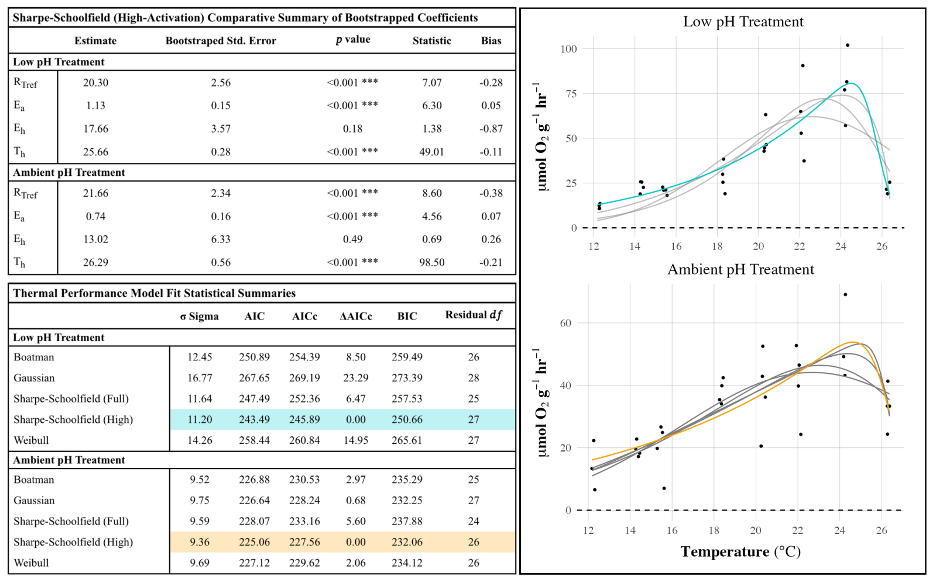
\includegraphics[width=5in]{figures/appendix/Appendix_5_Model_Selection.png}
\label{tab:appendixB4}
\end{table}

\newpage

\begin{table}[H]
\caption[Two-Way ANOVA for energetic expenditure.]{Two-Way ANOVA results for the role of temperature and pH on energetic expenditure (J g$^{-1}$ h$^{-1}$) in \textit{Tegula funebralis}. The table includes the main effects of Temperature Treatment, pH Treatment, and their interaction, with degrees of freedom (df), sum of squares (SS), mean squares (MS), $F$-Statistic, and $p$-value.}
\centering
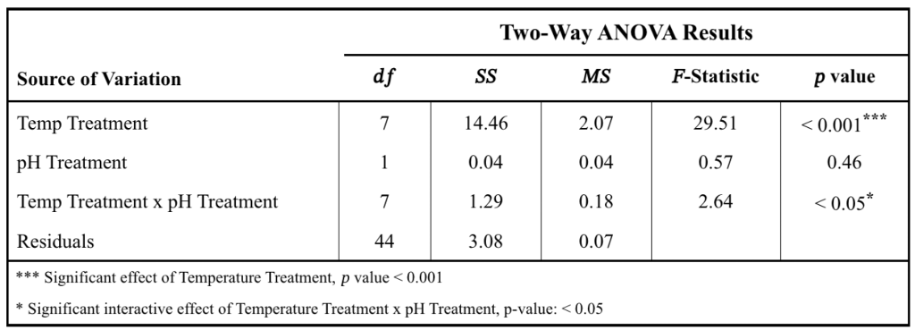
\includegraphics[width=5in]{figures/appendix/Appendix_6_Joule_ANOVA.png}
\label{tab:appendixB5}
\end{table}

\newpage

\begin{table}[H]
\caption[Pairwise energy expenditure differences across pH treatments.]{Energy expenditure of \textit{Tegula funebralis} (J g$^{-1}$ h$^{-1}$) across varying temperature treatments (12–26$^\circ$C) under ambient and low pH conditions. Pairwise comparisons between pH treatments were calculated using the estimated marginal means, with means ($\bar{x}$), standard errors ($\sigma_{\bar{x}}$), pairwise differences, 95\% confidence intervals, $t$-statistics, adjusted $p$-values (Bonferroni correction), and percent differences between treatments. Significant differences ($p < 0.05$) are noted.}
\centering
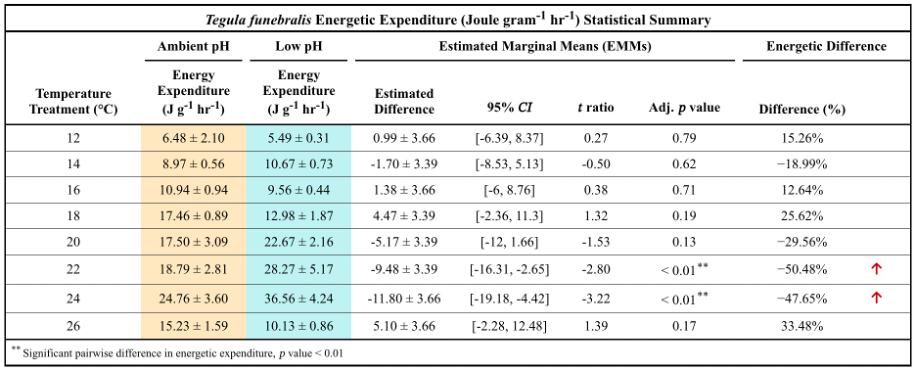
\includegraphics[width=5in]{figures/appendix/Appendix_7_J_Table.png}
\label{tab:appendixB6}
\end{table}

\backmatter

\end{document}
